%% Trying a small change

\documentclass{svproc}

% RECOMMENDED %%%%%%%%%%%%%%%%%%%%%%%%%%%%%%%%%%%%%%%%%%%%%%%%%%%

% to typeset URLs, URIs, and DOIs
\usepackage{url}
\def\UrlFont{\rmfamily}

% choose options for [] as required from the list
% in the Reference Guide

\usepackage{mathptmx}       % selects Times Roman as basic font
\usepackage{helvet}         % selects Helvetica as sans-serif font
\usepackage{courier}        % selects Courier as typewriter font
\usepackage{type1cm}        % activate if the above 3 fonts are
                            % not available on your system
%
\usepackage{makeidx}         % allows index generation
\usepackage{graphicx}        % standard LaTeX graphics tool
                             % when including figure files
\usepackage{multicol}        % used for the two-column index
\usepackage[bottom]{footmisc}% places footnotes at page bottom

\usepackage{breakcites}      %% To prevent line overflows due to many refs.



\newcommand{\partg}{\mbox{$\Pi_{G}$}}
\newcommand{\pgone}{\mbox{$\Pi_{G_1}$}}
\newcommand{\pgtwo}{\mbox{$\Pi_{G_2}$}}


\def\myendofproof{\vbox{\hrule\hbox{%
   \vrule height1.3ex\hskip0.8ex\vrule}\hrule}\par}
\newcommand{\set}[1]{\{ #1 \}}


\newcommand{\order}[1]{$\mbox{O}\left(#1\right)$}                   

\newcommand{\floor}[1]{\lfloor #1 \rfloor}
\newcommand{\lbound}[1]{$\Omega\left(#1\right)$}
\newcommand{\mod}[1]{\left| #1 \right|}
\newcommand{\abs}[1]{\mod{#1}}
\newcommand{\belongs}{$\in$}
\newcommand{\ceil}[1]{\left\lceil #1 \right\rceil}
\newcommand{\ith}{$i$th}
\newcommand{\npdt}{$\mbox{{\em NP}} 
                    \subseteq \mbox{{\em DTIME}}(n^{\log\log{n}})$}

\newcommand{\cals}{{\cal S}}
\newcommand{\calr}{{\cal R}}
\newcommand{\lp}[2]{
 \ \\
 \begin{tabular}{l} #1 \end{tabular}

 subject to constraints:

 \begin{tabular}{rcll} #2 \end{tabular}
 \ \\
}
\newcommand{\constraint}[4]{$#1$ & $#2$ & $#3$ &$#4$}
%  MACROS FOR ALGORITHMS OR PROGRAMS
\newcommand{\narrow}{\renewcommand{\baselinestretch}{.8}}
\newcommand{\wide}{\renewcommand{\baselinestretch}{1}}
\newcounter{program}
\newcounter{proglab}
\newcounter{proglabb}
\newcommand{\startstring}{}
\renewcommand{\theproglab}{\startstring\arabic{proglab}}
\renewcommand{\theproglabb}{\startstring\alph{proglabb}}

\setlength{\leftmarginii}{.4\leftmarginii}
\setlength{\leftmarginiii}{.4\leftmarginiii}
\setlength{\leftmarginiv}{.4\leftmarginiv}
\setlength{\leftmarginv}{.4\leftmarginv}

\newlength{\leftmarginsumii}
\newlength{\leftmarginsumiii}
\newlength{\leftmarginsumiv}
\newlength{\leftmarginsumv}
\setlength{\leftmarginsumii}{\leftmargini}
\addtolength{\leftmarginsumii}{\leftmarginii}
\setlength{\leftmarginsumiii}{\leftmarginsumii}
\addtolength{\leftmarginsumiii}{\leftmarginiii}
\setlength{\leftmarginsumiv}{\leftmarginsumiii}
\addtolength{\leftmarginsumiv}{\leftmarginiv}
\setlength{\leftmarginsumv}{\leftmarginsumiv}
\addtolength{\leftmarginsumv}{\leftmarginv}

\newlength{\itemindentvalue}
\setlength{\itemindentvalue}{0em}
\newenvironment{programi}%
{\narrow\begin{list}{\theproglab\hfill}{\usecounter{proglab}
		   \setlength{\topsep}{0pt}
		   \setlength{\itemsep}{0pt}
		   \setlength{\labelsep}{0pt}
		   \setlength{\labelwidth}{\leftmargini}
		   \setlength{\listparindent}{0pt}
		   \setlength{\itemindent}{\itemindentvalue}
		   \setlength{\leftmargin}{\leftmargini}}
 \setcounter{program}{0}
 \setcounter{proglab}{\value{program}}}%
{\end{list}\wide}

\newenvironment{programI}%
{\narrow\begin{list}{\theproglabb\hfill}{\usecounter{proglabb}
		   \setlength{\topsep}{0pt}
		   \setlength{\itemsep}{0pt}
		   \setlength{\labelsep}{0pt}
		   \setlength{\listparindent}{0pt}
		   \setlength{\labelwidth}{\leftmargini}
		   \setlength{\itemindent}{\itemindentvalue}
		   \setlength{\leftmargin}{\leftmargini}}
 \setcounter{program}{0}
 \setcounter{proglabb}{\value{program}}}%
{\end{list}\wide}

\newenvironment{programii}%
{\narrow\begin{list}{\theproglab\hfill}{\usecounter{proglab}
		   \setlength{\topsep}{0pt}
		   \setlength{\itemsep}{0pt}
		   \setlength{\labelsep}{0pt}
		   \setlength{\listparindent}{0pt}
		   \setlength{\labelwidth}{\leftmarginsumii}
		   \setlength{\itemindent}{\itemindentvalue}
		   \setlength{\leftmargin}{\leftmarginii}}
 \setcounter{proglab}{\value{program}}}%
{\end{list}\wide}

\newenvironment{programiii}%
{\narrow\begin{list}{\theproglab\hfill}{\usecounter{proglab}
		   \setlength{\topsep}{0pt}
		   \setlength{\itemsep}{0pt}
		   \setlength{\labelsep}{0pt}
		   \setlength{\listparindent}{0pt}
		   \setlength{\labelwidth}{\leftmarginsumiii}
		   \setlength{\itemindent}{\itemindentvalue}
		   \setlength{\leftmargin}{\leftmarginiii}}
 \setcounter{proglab}{\value{program}}}%
{\end{list}\wide}

\newenvironment{programiv}%
{\narrow\begin{list}{\theproglab\hfill}{\usecounter{proglab}
		   \setlength{\topsep}{0pt}
		   \setlength{\itemsep}{0pt}
		   \setlength{\listparindent}{0pt}
		   \setlength{\labelsep}{0pt}
		   \setlength{\labelwidth}{\leftmarginsumiv}
		   \setlength{\itemindent}{\itemindentvalue}
		   \setlength{\leftmargin}{\leftmarginiv}}
\setcounter{proglab}{\value{program}}}%
{\end{list}\wide}

\newenvironment{programv}%
{\narrow\begin{list}{\theproglab\hfill}{\usecounter{proglab}
		   \setlength{\topsep}{0pt}
		   \setlength{\itemsep}{0pt}
		   \setlength{\listparindent}{0pt}
		   \setlength{\labelsep}{0pt}
		   \setlength{\labelwidth}{\leftmarginsumv}
		   \setlength{\itemindent}{\itemindentvalue}
		   \setlength{\leftmargin}{\leftmarginv}}
\setcounter{proglab}{\value{program}}}%
{\end{list}\wide}

\newcommand{\progitem}{\addtocounter{program}{1}\item}
\newcommand{\calb}{{\cal B}}
\newcommand{\calc}{{\cal C}}
\newcommand{\calp}{{\cal P}}


% box for end of proof
\newcommand{\QED}{~~ \rule{2mm}{2mm}}

\newcommand{\n}{$n \,$}
\newcommand{\G}{$G \,$}
\newcommand{\Gi}{$G_i \,$}
\newcommand{\Gj}{$G_j \,$}
\newcommand{\Gz}{$G_0 \,$}
\newcommand{\Gn}{$G_n \,$}
\newcommand{\Go}{$G_1 \,$}
\newcommand{\Gt}{$G_2 \,$}
\newcommand{\Gth}{$G_3 \,$}
\newcommand{\Gnl}{$G_{n-1} \,$}
\newcommand{\Gil}{$G_{i-1} \,$}


\newcommand{\Hi}{$H_i \,$}
\newcommand{\Fi}{$F_i \,$}
\newcommand{\Fj}{$F_j \,$}
\newcommand{\Fz}{$F_0 \,$}
\newcommand{\Fk}{$F_k \,$}
\newcommand{\Fo}{$F_1 \,$}
\newcommand{\Ft}{$F_2 \,$}
\newcommand{\Fth}{$F_3 \,$}
\newcommand{\Fkl}{$F_{k-1} \,$}
\newcommand{\Fnl}{$F_{n-1} \,$}
\newcommand{\Fn}{$F_n \,$}


\newcommand{\fj}{$f_j \,$}

\newcommand{\ol}{ 1-level}
\newcommand{\kl}{$k$-level}
\newcommand{\hcally}{hierarchically \,}
\newcommand{\hcal}{hierarchical \,}
\newcommand{\CPSPACE}{PSPACE \,}
%\newcommand{\belongs}{$\in$}
%\newcommand{\ith}{$i$th}



\newcommand{\smallspacing}{\baselineskip = 0.7\normalbaselineskip}
\newcommand{\tinyspacing}{\baselineskip = 0.5\normalbaselineskip}
\newcommand{\morespacing}{\baselineskip = 1.1\normalbaselineskip}


% Commands for stacking.
\newcommand{\RMAX}{\max_{\stackrel{\{x,y\},x \neq y}{x,y \in P}}}
\newcommand{\RSUM}{\sum_{\stackrel{\{x,y\},x \neq y}{x,y \in P}}\!}


\newcounter{xalgcount}

\newcommand{\newspacing}{\baselineskip=1.1\normalbaselineskip}
\newcommand{\oldspacing}{\baselineskip= 1.0\normalbaselineskip}

\newspacing

\begin{document}

% ************ end of program macros *********************************
\title{Dichotomy Theorems for Hierarchical and 1-Dimensional Periodically Specified Boolean Constraint Satisfaction Problems}
\titlerunning{Dichotomy Theorems} 
% Use \titlerunning{Short Title} for an abbreviated version of
% your contribution title if the original one is too long
\authorrunning{Marathe~et~al.}

\author{ Madhav V. Marathe 
       \and{~} Harry B. Hunt III
        \and {~}Venkatesh Radhakrishnan   %%{\vspace*{-1.7in}}
       \and{\newline} S. S. Ravi
       \and  {~}Daniel J. Rosenkrantz
        \and {~}  Richard E. Stearns
}
\institute{
           Madhav V. Marathe: University of Virginia. 
           \email{marathe@virginia.edu}.  \and
          Venkatesh Radhakrishnan: Google
            \email{venky@gmail.com}.  \and
           H.~B. Hunt III, S. S. Ravi, D. J. Rosenkrantz, R. E. Stearns: 
           University of Virginia and University~at~Albany~--~SUNY.{\newline}
           \email{\{hunt,~ssravi0,~drosenkrantz,~thestearns2\}@gmail.com}.
}


\maketitle



\begin{abstract}
We study the complexity of various combinatorial and satisfiability problems
when instances are specified using one of the following succinct 
specifications:
(1) the 1-dimensional finite periodic narrow specifications 
(denoted by {\sf 1-FPN}-specifications)  of  
 Ford  et al. and Wanke \cite{FF58,Wa93};
(2) the 1-dimensional finite periodic narrow specifications with explicit
boundary conditions 
(denoted by {\sf 1-FPN(BC)}-specifications) of Gale \cite{Ga59}; 
and  
(3) the hierarchical specifications (denoted by {\sf L}-specifications)
of Lengauer et al. \cite{LW87a}.
First, we prove that there is a polynomial time algorithm that,
given a {\sf 1-FPN}- or {\sf 1-FPN(BC)}-specification of a graph 
(or a {\sf CNF} formula), constructs a level-restricted {\sf L}-specification
of an isomorphic graph (or formula). Second assuming {\sf P} $\neq$
 {\sf PSPACE},  we characterize completely the polynomial time 
solvability of the generalized {\sf CNF} satisfiability problems of 
Schaefer \cite{Sc78}, when instances are specified succinctly
as in (1), (2) or (3) above.
\end{abstract}


\section{Introduction}
\label{sec:intro}

Large objects with a highly repetitive structure can often be represented
succinctly.
In the past, several methods have been proposed to succinctly 
represent such objects.
Here we consider two of these methods, namely
(i) hierarchical specifications  
\cite{Ga82,GW83,LW92,BOW83,RH93,LW93,MH+93a,MH+94,marathe1995complexity,Wa86},
and (ii) periodic specifications 
\cite{CM91,HW92,IS87,KO91,KS88,Or82a,Wa93}.
 


Hierarchical specifications are useful in describing large scale systems with
very regular structures. 
Using hierarchical specifications, the overall design of an object can be 
partitioned into the design of a collection of modules;
this is a 
much more manageable task compared to producing a complete design in one step.
Such a top down (or hierarchical design) approach 
also facilitates the development of computer aided design (CAD) systems, since
low-level objects can be  incorporated into libraries and can thus be made
available as submodules to designers of large scale  objects.
Other areas where hierarchical specifications have found applications are
VLSI layout \cite{Le82,Le86,Le90,HLW92,HW92,RH93},  
finite element analysis, software engineering and Datalog queries 
(see \cite{HLW92,Ma94,marathe1995complexity,bottcher2020simulation,goller2005fixpoint,brenguier2012comparison,lohrey2012model,tapken1999implementing,AC94} 
and the references therein).  Recently, there has been interest in
inferring the inherent hierarchy that graphs might exhibit from the
standpoint of graph neural networks \cite{ying2018hierarchical}.

Periodic specifications
can also be used to define large scale systems with highly regular structures.
Using  periodic specifications, 
large objects are  described as repetitive connections of a basic module.
Frequently, the modules are connected in a straight line 
but the basic modules can also  be repeated in two or higher
dimensional patterns. Periodic specifications are also used to 
model time variant  problems,  where the constraints
or demands  for any one period is the same as those for preceding or 
succeeding periods. 
Periodic specifications 
have applications in such diverse areas  as  transportation planning
\cite{Or82a,HLW92,marathe1995complexity,drucker2019cyclic,ho2015cyclic},
parallel programming \cite{HLW92,KMW67} wireless networks 
\cite{andreou2002radiocoloring,fotakis2006radiocolorings} and 
VLSI design \cite{IS87,IS88}. 
See \cite{chen2003periodic,chen2005periodic} for a good discussion and 
references on periodic constraint satisfaction problems.

Orlin has studied periodically specified problems over an infinite 
horizon; i.e the objects considered are infinite \cite{Or82a}. 
Ford and Fulkerson \cite{FF58} and Wanke \cite{Wa93} have 
studied the finite horizon
versions of periodic problems and Gale \cite{Ga59} has studied problems for
periodic specifications with fixed starting points. All the above mentioned
studies are for 1-dimensional periodic specifications.
Other 
researchers have studied 2-dimensional and more generally $d$-dimensional
periodic specifications; 
see \cite{drucker2019cyclic,ho2015cyclic,CM91,IS87,KO91,KS88,Wa93}. 

An important feature of  both hierarchical and periodic 
specifications is that they
can be much  more concise in describing  objects than standard  specifications.
In general, the size of an object can be \emph{exponential} in the
size of its periodic or hierarchical specifications.
Since, the  complexity of solving a problem 
is usually measured as a function of the size of the specification of the 
problem instance,  
the complexity of a problem when instances are specified using
standard descriptions can
be  different than the complexity of the same problem 
when instances are specified hierarchically or periodically.
For example, while the {\sf 3-COLORING} problem is 
{\sf NP-}complete when the graphs are represented by adjacency matrices
or by adjacency lists \cite{GJ79}, it is 
{\sf PSPACE}-complete when instances are specified
hierarchically or periodically \cite{LW92,Or84b}.
On the other hand, the {\sf 2-COLORING} problem is solvable in polynomial time
{\em even} when instances are specified by the hierarchical
specifications of Lengauer et al. \cite{LW92,LW87a} or by  the 
1-dimensional periodic specifications of Orlin \cite{Or82a}.




In this paper, we study the complexity of combinatorial, graph and 
generalized {\sf CNF} satisfiability problems,
when instances are specified in any of the following ways:

\begin{enumerate}
\item
the 1-dimensional finite periodic narrow specifications (denoted by
{\sf 1-FPN}-specifications) of Ford and Fulkerson \cite{FF58}
and of Wanke \cite{Wa93}; 
\item
the 1-dimensional finite periodic narrow specifications with explicit 
boundary conditions (denoted by {\sf 1-FPN(BC)}-specifications)
of Gale \cite{Ga59} and others; 
\item
the 2-way infinite 1-dimensional narrow
periodic (sometimes called dynamic) specifications  (denoted by
{\sf 1-PN}-specifications) 
of Karp et al. and Orlin \cite{KMW67,Or82a}; and 
\item
the hierarchical specifications (denoted by {\sf L}-specifications) of 
Lengauer \cite{LW87a}. 
\end{enumerate}

\noindent
Let $\Pi$ be a problem, whose instances are specified {\em non-succinctly} 
using one of the standard specifications in the literature. For example,
instances of {\sf CNF} satisfiability problems can be specified non-succinctly
by {\sf CNF} formulas and by sets of clauses, with each clause being a set of 
literals.
Here, we use {\sf 1-FPN-}, {\sf 1-FPN(BC)-}, {\sf 1-PN-} and {\sf L-}$\Pi$ to
denote the problem $\Pi$ 
when its instances are specified succinctly by {\sf 1-FPN-}, 
{\sf 1-FPN(BC)-}, {\sf 1-PN-} and {\sf L-} specifications, respectively. 
We use $\alpha$-$\Pi$ to denote the problems {\sf 1-FPN-}, {\sf 1-FPN(BC)-},
 {\sf 1-PN-} and {\sf L-}$\Pi$; and we use {\em succinct} specification 
to mean {\sf 1-FPN-}, {\sf 1-FPN(BC)-}, {\sf 1-PN-} and {\sf L-}specification. 
Thus for example, {\sf 1-FPN-3SAT} denotes the problem {\sf 3SAT}
when instances are specified  by {\sf 1-FPN-}specifications; and 
$\alpha$-{\sf 3SAT} denotes the problems {\sf 1-FPN-}, {\sf 1-FPN(BC)-}, 
{\sf 1-PN-} and {\sf L-3SAT}.

\smallskip

Our results are summarized in the next section.


\section{Summary of Results}
\label{sec:summary}

The rest of the paper is organized as follows.  In Subsections 
\ref{sec:trans} through \ref{sec:comp} 
we summarize our  results and discuss their relationship with related 
results in the literature. Section \ref{sec:def} gives both the 
definitions and examples of the kinds of  succinct 
specifications considered in this paper.
In Section \ref{sec:translation}
we  prove a translation theorem  relating the 
{\sf 1-FPN-} and {\sf 1-FPN(BC)-}specifications 
to equivalent {\sf L-}specifications. 
 In Section \ref{sec:hard_3sat},
we prove the {\sf PSPACE}-hardness of the problems
\begin{quote}
 {\sf 1-FPN-3SAT}, {\sf 1-FPN(BC)-3SATWP},  {\sf L-3SAT}, and
{\sf L-3SATWP}.
\end{quote}
In Section \ref{sec:poly} we discuss several kinds of  
{\sf L-} and {\sf 1-FPN-}specified generalized {\sf CNF} 
 satisfiability problems that are solvable in 
polynomial time. In Section \ref{sec:char} 
we complete the characterization of the polynomial time solvability
of the problems $\alpha-${\sf SAT(S)}, assuming that {\sf P}$\neq${\sf PSPACE}. 
%%%%
%%%% The current version does not include proofs of the results mentioned below.
%%%%
%% In  Section \ref{sec:applications}, 
%% we outline how efficient reductions involving local replacement \cite{GJ79}
%% of the problems {\sf 3SAT, Planar 3SAT, 3SATWP,} etc., can be extended 
 %% to efficient reductions of the corresponding problems 
%% $\alpha$-{\sf 3SAT}, $\alpha$-{\sf Pl-3SAT}, $\alpha$-{\sf 3SATWP}, etc. 
%% This enables us to prove  the {\sf PSPACE-}hardness of a number of 
%% {\sf P-} and {\sf NP-}hard problems in the literature when instances are
%% specified succinctly, including the various {\sf PSPACE-}hard problems 
%% for {\sf 1-PN-}specifications in \cite{Or82a} and for {\sf L-}specifications
%% in \cite{LW92}. 

 
%\vspace*{-0.15in}
\subsection{Translation Theorem}\label{sec:trans}

In Theorem 4.1(called the {\bf Translation Theorem}),
we prove that a {\sf 1-FPN-} or {\sf 1-FPN(BC)-} specification of a graph
or  formula can be translated in polynomial time into an
{\sf L}-specification of an isomorphic  graph or formula, respectively.
This theorem implies that for many problems
$\Pi$ including all problems considered here,  the problems 
{\sf 1-FPN-} or {\sf 1-FPN(BC)-}$\Pi$ are 
polynomial time reducible to  the problem {\sf L-}$\Pi$.

%\vspace*{-0.15in}
\subsection{Complexity of Boolean Constraint Satisfaction Problems}\label{sec:sat}

In Sections \ref{sec:hard_3sat} through \ref{sec:char}, we study
the complexities of the generalized {\sf CNF}  satisfiability
problems {\sf SAT(S)} of \cite{Sc78}, when instances are specified
succinctly.  (A definition of {\sf SAT(S)} is given in
Section~\ref{sec:def}.) Assuming {\sf P} $\neq$ {\sf PSPACE}, we
characterize completely the polynomial time solvability of the
problems  $\alpha$-{\sf SAT(S)} as follows. We give sufficient
conditions on a finite set {\sf S} of finite-arity Boolean relations
for the problem  $\alpha$-{\sf SAT(S)} to be {\sf PSPACE-}complete.
We also show, for all such {\sf S} {\em not} satisfying these
conditions, that the problem $\alpha$-{\sf SAT(S)} is polynomial
time solvable. 
As a step in obtaining this characterization,
we prove in Section 6 
that the problems {\sf 1-FPN-3SAT}, {\sf 1-FPN(BC)-3SATWP},
and {\sf 1-FPN(BC)-3SATWN} are {\sf PSPACE-}hard. By the Translation
Theorem, this implies that the problems {\sf L-3SAT}, {\sf L-3SATWP},
and {\sf L-3SATWN} are also {\sf PSPACE-}hard.

%\vspace*{-0.15in}
\subsection{A Step Towards a Complexity Theory for Succinctly Specified 
Problems}
In Section~\ref{sec:conclusion}, we briefly outline how a 
polynomial time reduction involving
local replacement \cite{GJ79} from the problem 
{\sf 3SAT, NAE 3SAT, Pl-3SAT,} etc., to a problem $\Pi$ can be extended
to obtain a polynomial time reduction from the corresponding problem 
$\alpha$-{\sf 3SAT}, $\alpha$-{\sf NAE 3SAT} ,
 $\alpha$-{\sf Pl-3SAT}, etc., to the problems
 $\alpha$-$\Pi$. Together with the results outlined in 
Sections 2.1 and 2.2, this enables us to do the following:
\begin{enumerate}
\item derive alternative and unified proofs of the {\sf PSPACE-}hardness 
results for {\sf 1-PN-} specifications in \cite{Or82a} and for
 {\sf L-}specifications in \cite{LW92}; and 
\item derive several new {\sf PSPACE-}hardness results for succinctly 
specified problems. 
\end{enumerate}

Often, our {\sf PSPACE-}hardness  proofs involve 
reductions that are more time and/or space efficient than those in 
\cite{Or82a,LW92}. Many of these hardness results hold, even when 
restricted to specifications of $O(\log {\cal N})$ 
bandwidth-bounded planar graphs.
 



%\vspace*{-0.15in}
\subsection{Comparison with Related Work}\label{sec:comp}
Orlin \cite{Or82a} proved that the problem {\sf 1-PN-3SAT} is 
{\sf PSPACE-}complete. He used this and known reductions from {\sf 3SAT} 
to prove the {\sf PSPACE-}hardness of the problems 
\begin{quote}
{\sf 1-PN-KNAPSACK, 1-PN-HAMILTON-PATH(1-PN-HP), 1-PN-3COLORING,} and 
{\sf 1-PN-3DM}.
\end{quote}
Wanke \cite{Wa93} has also proved {\sf PSPACE-}hardness results for periodically-specified problems; but his results do not hold for 1-dimensional 
periodically-specified problems. Lengauer and Wagner \cite{LW92} proved
the {\sf PSPACE}-hardness of the problems 
\begin{quote}
{\sf L-3COLORING, L-INDEPENDENT SET(L-IS), L-HAMILTON CIRCUIT(L-HC), L-MONOTONE CIRCUIT  VALUE PROBLEM(L-MCVP), L-NETWORK FLOW(L-NF),} and {\sf L-ALTERNATING GRAPH ACCESSIBILITY PROBLEM(LAGAP).}
\end{quote}
Their {\sf PSPACE-}hardness results for the problems {\sf L-3COLORING, L-IS,}
and {\sf L-HC} hold for $O(\log {\cal N})$ bandwidth-bounded instances. Several
{\sf PSPACE-}hardness results for {\sf L-}specified unit disk graphs were 
presented in our paper \cite{MR+93}. 
Our results extend the results above from \cite{Or82a,LW92}  
in the following ways:

%%\begin{enumerate}
%%\item 
\noindent
1.~ Previously, the complexities of periodically- and hierarchically-specified
problems have been studied separately. Our results show that there is a
 close correspondence between Orlin's {\sf PSPACE-}hardness results for {\sf 
1-PN-}specified problems and Lengauer and Wagner's {\sf PSPACE-}hardness 
results for {\sf L-}specified problems.

\smallskip
\noindent
2.~
The only previous work on the complexities of the problems 
$\alpha$-{\sf SAT(S)} is that of Orlin \cite{Or82a} on the 
{\sf PSPACE-}hardness of the problem {\sf 1-PN-3SAT}. (Several references
to the results in this paper occur in our paper \cite{MR+93}.)

\smallskip
\noindent
3.~
No {\sf PSPACE-}hardness results, for succinctly presented 
planar problems, have been presented previously. No {\sf PSPACE-}hardness 
results of any kind have been presented previously, for problems specified
by either {\sf 1-FPN-} or {\sf 1-FPN(BC)-}specifications.

\smallskip
\noindent
4.~
Our {\sf PSPACE-}hardness results for {\sf L-}specified
problems imply the {\sf PSPACE-}hardness of the problems 
{\sf L-MCVP} and {\sf L-AGAP} for $O(\log {\cal N})$ 
bandwidth-bounded instances.

\smallskip
\noindent
5.~
Several of our  reductions  used to prove {\sf PSPACE-}hardness
are more  efficient in both   time  and space than  the  corresponding
reductions in \cite{Or82a,LW92}. For example,   our proof of the  {\sf
PSPACE-}hardness  of  {\sf  1-PN-3SAT}  is   by an  $O(n\log n)$  time
reduction of the acceptance problem  for a nondeterministic {\sf LBA}.
The proof by Orlin \cite{Or82a} uses  an $\Omega(n^2 \log n)$  time  and
space reduction  of the same  problem. Under the  plausible assumption
that  there exist   {\sf  LBA}s   whose acceptance  problems   require
$2^{\Omega(n)}$ time  on deterministic Turing machines,  our reduction
implies    that     the    problem     {\sf    1-PN-3SAT}     requires
$2^{\Omega(n/\log{n})}$   time  on   deterministic    Turing
machines. Orlin's reduction only  implies that the problem {\sf 1-PN-3SAT}
requires   $2^{\Omega(\sqrt{n}/{\log {n}})}$ time on deterministic
Turing machines.

\smallskip
\noindent
6.~
Our proofs show that it is possible to use knowledge 
about {\em local reductions} from generalized {\sf CNF} satisfiability problems
in the standard case to predict the complexity of problems when instances
are succinctly specified. 

%% Commented out as the discussion is not in Section 8.
%% We discuss points 5 and 6 in greater detail in Section 8.
%\end{enumerate}


\section{Definitions and Preliminaries}\label{sec:def}

Subsections  \ref{sec:other_def} through \ref{sec:fpn_spec} give
basic definitions used here, including the definitions of the
generalized {\sf CNF} Satisfiability problems  of \cite{Sc78} and
the kinds of succinct specifications considered. We illustrate these
definitions with several examples.


%%\vspace*{-0.15in}
\subsection{The Problems {\sf SAT(S)}}\label{sec:other_def}

We first review some basic definitions  from Schaefer \cite{Sc78}.

\begin{definition}\label{s-formulas:def}(Schaefer \cite{Sc78})\\
Let S $= \{R_1,R_2, \cdots, R_m \}$ be a finite 
set of finite arity Boolean
relations. (A Boolean relation is defined to be 
any subset of $\{0,1 \}^p$ for some integer $p \geq 1$. 
The integer $p$ is called the  {\bf rank} of the relation.)
An S-{\it formula} is a conjunction of clauses each of the form 
$\hat{R}_i(\xi_1, \xi_2, \cdots)$, where $\xi_1, \xi_2, \cdots$ are distinct, 
unnegated variables whose number matches the 
rank of $R_i, i \in \{ 1, \cdots m \}$ and $\hat{R}_i$ is the relation symbol
representing the relation $R_i$.
The  S-{\it Satisfiability problem} (denoted by SAT(S)) 
is the problem of deciding 
whether a given S-formula is satisfiable.

The problem {\sf SAT$_c$(S)} is the variant of the problem 
{\sf SAT(S)} in which the constants $0$ and $1$ are also allowed
to occur in {\sf S-}formulas. 
\end{definition}


The 
generalized {\sf CNF} Satisfiability problems {\sf SAT(S)} and 
{\sf SAT$_c$(S)} generalize  the problem  {\sf 3SAT} and its variants
studied in the literature \cite{GJ79}. For example,
let $R(x,y,z)$ be the ternary logical relation  given by
$\{(1,0,0), (0,1,0), (0,0,1) \}$. Then, the problem 
{\sf 1-3SAT}  is the same as the problem {\sf SAT(\{R\})}. 

\iffalse
Similarly, {\sf NAE3SAT} is the problem of determining if
a {\sf 3CNF} formula, has a satisfying assignment in which all the literals
in any clause are not simultaneously true. 
\fi



\begin{definition}\label{def:affine}

\begin{enumerate}
\item
The logical relation $R$ is {\bf 0-valid} if $(0, \ldots, 0) \in R$.
\item
The logical relation $R$ is {\bf 1-valid} if $(1, \ldots, 1) \in R$.
\item
The logical relation $R$ is {\bf weakly positive} if
$R(x_1,x_2,\ldots)$ is logically equivalent to some CNF formula having at
most one negated variable in each conjunct.
\item
The logical relation $R$ is {\bf weakly negative} if
$R(x_1,x_2,\ldots)$ is logically equivalent to some CNF formula having at
most one unnegated variable in each conjunct.
\item
The logical relation $R$ is {\bf bijunctive} if
$R(x_1,x_2,\ldots)$ is logically equivalent to some CNF formula having at
most two literals in each conjunct.
\item
The logical relation $R$ is {\bf affine} if $R(x_1,x_2,\ldots)$ is logically 
equivalent to some system of linear equations over the two-element field 
${\bf Z}_2$.
\item
The logical relation $R$ is {\bf complementive} 
if it is closed under component-wise
complement; i.e., for all $(a_1,\ldots,a_m)$, if $(a_1,\ldots,a_m) \in R$, 
then $(1-a_1,\ldots,1-a_m) \in R$.
\item
The logical relation $R$ is {\bf 1-weakly positive} if
$R(x_1,x_2,\ldots)$ is logically equivalent to some CNF formula having at
most one negated variable in each conjunct, such that any clause with
a negated literal has no more than 1 unnegated literal.
\item
The logical relation $R$ is {\bf 1-weakly negative} if
$R(x_1,x_2,\ldots)$ is logically equivalent to some CNF formula having at
most one unnegated variable in each conjunct, such that any clause with
an unnegated literal has no more than 1 negated literal.
\end{enumerate}
\end{definition}



\begin{definition}\label{def:rep}
(1)~ If $A$ is a formula, then we denote the 
logical relation defined by $A$ as {\bf $[A]$},
when the variables are taken in ascending order.

\noindent
(2)~ {\sf $Gen(S)$} is the set of existentially quantified $S$-formulas with
constants.

\noindent
(3)~ {\sf $Rep(S)$} is the set of relations that are representable by existentially 
quantified $S$-formulas with constants.

\noindent
(4)~ {\sf $Rep_{NC}(S)$} is the set of relations that are 
representable by existentially quantified $S$-formulas without constants.
\end{definition}




%%\vspace*{-0.15in}
\subsection{The L-Specified Formulas}\label{sec:lspec}
We define the terminology for {\sf L-}specified generalized {\sf CNF} formulas used here. 
%\subsubsection{L-specified S formulas}\label{sec:hsat_def}
Let $S$ be a finite nonempty set of finite-arity Boolean 
relations. The definitions of L-specification of an S-formula, the 
S-formulas specified by such specifications, and the problems 
{\sf L-SAT(S)} and {\sf L-SAT}$_c${\sf (S)} are closely analogous to Definitions
3.5, 3.6 and 3.1, respectively.

\begin{definition}
Let $X$ be a vector of Boolean variables and the constants $0$ and $1$. Then
$\hat{X}$ is the set of all variables occurring in $X.$
\end{definition}

\begin{definition}\label{hsats:def}
An {\sf L-}specification $F(X) = (A_1(X_1),\ldots, A_n(X_n))\, (n \geq 1)$ 
of an S-formula (or of an S-formula with constants) is a finite nonempty 
sequence of assignment statements $A_i(X_i)$ of the form 
\[ F_i(X_i) \leftarrow 
(\bigwedge_{1 \leq k \leq  l_i} F_{i_k}(X_{i_k},Z_{i_k})) \bigwedge 
f_i(X_i,Z_i), \]
where, for $1 \leq i_k \leq l_i$,\\
(1) $1 \leq i_k < i,$ \\
(2) $X_i, X_{i_k}, Z_i$ and $Z_{i_k}$ are vectors of Boolean variables (or are 
vectors of Boolean variables, $0$, and $1$) respectively; and \\
(3) $X = \hat{X},~ \hat{X}_{i_k} \subseteq \hat{X_i},$ ~and~ $ \hat{Z_{i_k}} 
\subseteq \hat{Z_i}$. 

\smallskip

\noindent
For $1 \leq i \leq n$, letting $\lambda_i$ be the number of occurrences of
literals in the statement $A_i$, the {\em size} of $F(X)$ denoted 
{\em size($F(X))$}, equals $\sum_{i=1}^{n} \lambda_i + n$.
\end{definition}

Given Definition \ref{hsats:def}, the definition of the 
{\sf S-formula} (or of the {\sf S}-formula with constants) 
$E(F(X))$ specified
by such an  L-specification $F(X)$ very closely follows Definition 3.6 and 
is not repeated here. 





\begin{example}
Let $F= (F_1(x_1,x_2),F_{2}(x_3,x_4), F_3)$
be an instance of {\sf L-3SAT} where each $F_i$ is defined as follows:
\[F_1(x_1,x_2) = (x_1 + x_2 + z_1) \wedge (z_2 + z_3) \]
\[F_2(x_3,x_4) = F_1(x_3, z_4) \wedge F_1(z_4, z_5) \wedge
                               (z_4 + z_5 + x_4)   \]
\[F_3 = F_2(z_8,z_7) \wedge  F_1(z_7,z_6) \]
The formula $E(F)$ denoted by $F$ is given by 
$ (z_7 + z_6 + z_1^1) \wedge (z_2^1 + z_3^1) \wedge
(z_8 + z_4 + z_1^2) \wedge (z_2^2 + z_3^2) \wedge $
$(z_4 + z_5 + z_1^3) \wedge (z_2^3 + z_3^3) \wedge (z_4 + z_5 + z_7)$. 

\end{example}


\begin{definition}
The problem {\sf L-SAT(S)} (or {\sf L-SAT}$_c${\sf (S)}) is the
problem of determining, given an L-specification $F(X)$ of the S-formula(or of
the S-formula with constants), if ${\cal F}(F(X))$ is satisfiable.
\end{definition}
 






%%\vspace*{-0.15in}
\subsection{Periodic Specifications }\label{sec:fpn_spec}
Next, we recall the definition of one dimensional periodic specifications 
due to  Orlin \cite{Or82a}, Wanke \cite{Wa93} and 
H\"ofting and Wanke \cite{HW92}. 
In the remainder of this paper, {\bf N} and {\bf Z} re used to 
denote the sets of non-negative integers and integers respectively.



%%\vspace*{-0.15in}
\subsubsection{Periodically Specified Formulas}

Earlier in this section, we extended
the definition of Satisfiability problems when instances are specified
by standard specifications so as to apply to 
{\sf L}-specified Satisfiability problems. Orlin \cite{Or82a} 
defined the problem {\sf 1-PN-3SAT}, that is, the problem {\sf 3SAT} when 
instances are specified using {\sf 1-PN}-specifications.
Here we define {\sf 1-FPN}- and {\sf 1-PN}-specified generalized Satisfiability
problems.




Let $U = \{u_1, \ldots, u_n \}$  be a finite set of variables (referred to
as static variables).
Further, let
$U^{\infty} =  \{u_k(i): ~ 1 \leq k \leq n, ~ i \in {\bf Z}\}$ and 
$U^{M} =  \{u_k(i): ~ 1 \leq k \leq n, ~ i \in \{0,1, 2, \cdots, M\}\}$. 
In our proofs, variable $u_k(i)$
denotes the variable $u_k$ at time unit $i$. 
A literal of $U$ is an element of 
$\{u_1, \ldots, u_n, \overline{u_1}, \ldots, \overline{u_n} \}$.
If $w$ is a literal of $U$, then $w(i)$, 
is a literal of $U^{\infty}$.
Let $C(i, i+1)$ be a parameterized conjunction of 3 literal clauses
such that each clause in $C(i, i+1)$ 
consists of variables $u_k(i), u_k(i+1)$ with the constraint that at least one
variable is of the form $u_k(i)$. 
We refer to the clauses $C(i, i+1)$ as  {\em static narrow clauses}. 
($C(i, i+1)$ is called  narrow because
for all  $(w_1(i_1) \vee w_2(i_2) \vee w_3(i_3)) \in C(i,i+1) $, 
$|i_s - i_r| \leq 1$ for $1 \leq r \leq s \leq 3$.)
Let $C^{\infty}$ $= \bigwedge_{i = 0}^{i =\infty}C(i, i+1)$. 
Given $U^{M}$ and $C^{\infty}$, let $C^{M}$ be a subset of $\cal C$ 
with the following property: for each clause 
$(w_1(i_1) \vee w_2(i_2) \vee w_3(i_3))  \in C^{M}$,
$ w_1(i_1), w_2(i_2), w_3(i_3) \in U^{M}$.



It is useful to imagine a narrow periodically specified formula
$\Gamma^{\infty}$ as being obtained by placing a copy of the variable 
set $U$
at each integral point (also referred to as time unit) 
on the X-axis (or the time line). 
Furthermore, assume that the clauses $C(t, t+1)$ are placed at time $t$.
With this notation, we can now refer to variables $U(t)$
as the set of variables at time $t$ 
and the clauses $C(t, t+1)$ as the set of clauses at time $t$.




\begin{definition}\label{fpn:sat}
A 1-dimensional infinite (finite) 
periodic narrow specification (denoted by 1-PN (FPN)-specification)
of a  3CNF formula  $F^{\infty}(U^{\infty}, C^{\infty})$
($F^{M}(U^{M}, C^{M})$) is given by 
($~\Gamma = (U,C(i,i+1))$,  ($~\Gamma = (U,C(i, i+1), M)$),  
where $U$ is  a finite set of variables and
$C(i, i+1)$ is a collection of static narrow 3 literal clauses. 
(In case of finite specifications $M$ is a non-negative integer 
specified in binary.)
The size of the specification denoted by 
$size(\Gamma) = |U| + |C(i, i+1)| $. (In case of finite specifications
$size(\Gamma)$ = $|U|$ $+ |C(i, i+1)|$ $+ bits(M)$,  
where $bits(M)$ denote the number
of bits used to represent $M$.)

\smallskip

The problem 1-PN-3SAT (i.e., problem 3SAT when instances are specified using 
1-FPN-specifications)  is the problem of determining if a 3CNF formula
$F^{\infty}(U^{\infty}, C^{\infty})$ specified by $\Gamma= (U,C(i, i+1))$ 
is satisfiable.

\smallskip

Similarly, the problem 1-FPN-3SAT (i.e., problem 3SAT specified using 
1-FPN-specifications)  is the problem of determining if a 3CNF formula
$F^{M}(U^{M}, C^{M})$ specified by $\Gamma$ = $(U,C(i, i+1),M)$ 
is satisfiable.
\end{definition}


For each finite set {\sf S} of finite arity Boolean relations, 
it is straightforward to extend the above 
definition so as to define the problems {\sf 1-PN-SAT(S)}  
and {\sf 1-FPN-SAT(S)};  hence, we omit those
definitions.  Observe that 
{\sf 1-FPN}-specified graphs or formulas can be exponentially larger 
than their input specifications. Finally, as in the previous subsection, 
we use ${\cal N}$ to denote the size of the formula $F^m(U^m, C^m)$ represented
using standard (non-succinct) specifications.

\smallskip
	 
\noindent
{\bf Example 4:}
Let $F= (U,C(i, i+1),3)$ be an instance of  {\sf 1-FPN-3SAT} 
where the set of static clauses are given by
$(x_1(i) + x_2(i) + x_3(i) )  \wedge 
(x_1(i+1) + x_3(i)) \wedge (x_3(i+1) + x_2(i))$.
The set of variables $U = \{ x_1, x_2, x_3 \}$.
The formula $F^3(U^3,C^3)$ denoted by $\Gamma$ is given by 
\[(x_1(0) + x_2(0) + x_3(0)) \wedge (x_1(1) + x_3(0)) \wedge (x_3(1) + x_2(0)) 
\bigwedge \]
\[(x_1(1) + x_2(1) + x_3(1)) \wedge (x_1(2) + x_3(1)) \wedge (x_3(2) + x_2(1)) 
\bigwedge \]
\[(x_1(2) + x_2(2) + x_3(2)) \wedge (x_1(3) + x_3(2)) \wedge (x_3(3) + x_2(2)) 
\bigwedge \]
\[(x_1(3) + x_2(3) + x_3(3)).\] \hfill\QED



%%\vspace*{-0.15in}
\subsubsection{1-FPN(BC)-specified Graphs and Formulas.}~
Some instances of problems arising in practice involve a periodic specification
of the graph or a formula along with explicit initial and final conditions.
We refer to such periodic specifications as periodic specifications with boundary
conditions ({\sf BC}). 
Observe that for {\sf 1-PN}-specifications boundary conditions
do not make sense since the expanded graph or the formula is infinite.
Hence boundary conditions are used to augment only {\sf 1-FPN}-specifications.

In such a case, we have a parameterized set of variables $V(i)$.
We place a copy of the variables from time $\{ 0, \cdots, m \}$.
We also have explicit variables $INIT$ and $FIN$ 
representing the variables at the
two boundaries. There are three sets of clauses.
The set of explicit clauses $C_1(INIT, V(0))$ contain variables from 
$INIT \cup V(0)$  with the constraint that at least one variable in each clause
is from the set $INIT$. Then we have the parameterized set of clauses
$C_2(i, i+1)$ which are identical to the clauses used to specify 
{\sf 1-FPN}-formulas. They contain variables from $V(i) \cup V(i+1)$.
Finally we have explicit clauses $C_3(V(m), FIN)$ which contain variables from
$FIN \cup V(m)$. 
The specification of the {\sf 1-FPN(BC)-CNF}-formula is given by
$\Gamma = ( F, m)$, where 
\[F = C_1(INIT, V(0) \cup C_2(V(i) \cup V(i+1)) \cup C_3(V(m) \cup FIN). \]
The formula specified by $\Gamma$ is given by 
\[E(\Gamma) =  
C_1(INIT, V(0)) \bigwedge \bigwedge_{i = 0}^{ i = m} C(i, i+1) \bigwedge 
C_3(V(m), FIN).  \]


\section{Translation Theorem}\label{sec:translation}


\begin{theorem}\label{th:translate}
There is a polynomial time transformation, that maps a 
1-FPN(BC)-specification $\Gamma = (G(V,E), m)$ of the  graph $\Gamma^m$ 
to a strongly 1-level-restricted 
L-specification $\Gamma_1$ of a graph, 
such that the graphs represented by 
$\Gamma$ and $\Gamma_1$ are isomorphic and 
$size(\Gamma_1) = (size(\Gamma))^2$.
\end{theorem}

\noindent
{\bf Proof:} We discuss the transformation without boundary conditions first.
Given a {\sf 1-FPN}-specification  $\Gamma = G(V,E)$ of $G^m$ 
we construct a {\sf L}-specification $H_G = (H_1, \cdots H_n)$ as follows. 
The non-terminal $H_1$  consists of four copies of $G$ (i.e. $G^4$). 
They are connected in series as shown in Figure \ref{translation1.fig}(a), 

%\iffalse
%%%%
\begin{figure}[tbh]
\centering
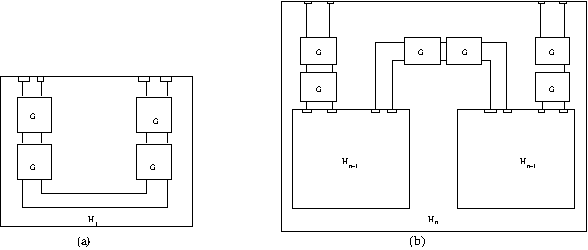
\includegraphics{translation1}
\caption{Construction of $H_i$, $1 \leq i \leq n$}
\label{translation1.fig}
\end{figure}
%%%%
%\fi




\noindent 
{\bf Non-terminal  $H_i$, $2 \leq i \leq n$:}
Asssume that the periodic graph is of the form $G^{2k}$.
The non-terminal $H_i$ consists of five components
$l_i$, $r_i$, $m_i$, $H_{i-1}$, $H_{i-1}$. 
Each of $l_i$, $r_i$ and  $m_i$ consists of at least 2 copies of $G$ 
($G^2$) attached in a manner as shown in the Figure \ref{translation1.fig}(b). 

Each $H_{i-1}$ recursively encodes $G^{p}$, 
We need to ensure that for each recursive
call $p$ is even, thus we need to adjust the sizes of 
the components $l_i$, $r_i$ and  $m_i$ accordingly.
The $H_{i-1}$'s 
are connected to the components $l_i$, $r_i$ and  $m_i$ as shown in 
Figure \ref{translation1.fig}(b). 
The condition that each $H_{i-1}$ have even number of copies of $G$ 
implies that the construction should satisfy the following constraints.
\[ |l_i|, ~ |r_i|, ~  |m_i| \geq 2 \]  
\[~~~ p = 2m \] 
\[2m + 2m + |l_i| + |r_i| +  |m_i| = 2k \]  


The first constraint is needed so that the resulting specification is 
1-level-restricted. The second equation says that $p$ is even. This is needed 
so that each of the smaller indexed non-terminals  
can be defined recursively. 
The third equation says that the 
total number of copies of $G$ is no more than $2k$, which is the size of the
graph we want to encode. It is clear that the sizes of $l_i$, 
$r_i$ and $m_i$ can be chosen  so that the above equations can be satisfied.
The process can be
carried out recursively to obtain the required specification $H$
in polynomial time.

Observe that a similar transformation can be carried out if we start
with a {\sf 1-FPN(BC)} specified graph $G$. 
In this case the graphs which specify the boundary conditions
are included in the highest non-terminal.\QED

Using similar ideas we can transform {\sf 1-FPN}-specified formulas into
isomorphic {\sf L}-specified formulas. Thus we have the following corollary.


\begin{corollary}\label{cor:translate}
There is a polynomial time transformation that maps a 
1-FPN(BC)-specification $\Gamma = (U, C(i, i+1), m)$ of the formula $\Gamma^m$ 
to a strongly 1-level-restricted 
L-specification $\Gamma_1$ such that
that the formulas represented by $\Gamma$ and $\Gamma_1$ are isomorphic and
$size(\Gamma_1)= O((size(\Gamma))^2)$ 
\end{corollary}


\section{PSPACE-completeness of $\alpha$-3SAT}\label{sec:hard_3sat}

\begin{theorem}\label{th:fpn-3sat}
%%\begin{enumerate}
(1) 1-FPN-3SAT is in NSPACE(n).~
(2) There is a $\theta(n)$ size 
quasi linear time reduction from the membership problem
for  non-deterministic linearly space bounded machine (LBA) 
to the problem 1-FPN-3SAT. 
Thus 1-FPN-3SAT is {\sf PSPACE}-complete. 
%%\end{enumerate}
\end{theorem}

\noindent
{\bf Proof:}  See supplementay material. 
\iffalse
%%%%%%%%%%%%%%%%%%%%%%%%%%%%%%%%%%%%%%%
{\em Part (1):}
We first show that the problem is in {\sf NSPACE($n$)}.
Observe that given a {\sf 1-FPN}-specification 
$\Gamma = (G(V,E), m)$, a Turing machine 
needs to maintain at any given time $t$ 
only assignments to variables at time $t$ and time $t+1$. 
Hence a non deterministic {\sf LBA}
can verify that the instance of {\sf 1-FPN-3SAT} is satisfiable as follows. At 
each step $t$ it guesses an assignment to the variables at grid point $t+1$.
It also remembers the assignment to the variables at grid point $t$. Using
these values it verifies that the clauses at time $t$ are indeed satisfied.
The number of time steps  $m$ can be kept track of using a counter of size
$O(m)$ (since $m$ is specified as a binary numeral). 
This proves that given an instance $\Gamma$ 
of {\sf 1-FPN-3SAT}, we can recognize in 
non-deterministic {\em linear } space (i.e in space $O(size(\Gamma))$) 
if the formula $G^m$ is satisfiable.

\noindent
{\em Part (2):}
Next, we prove {\sf 1-FPN-3SAT} is {\sf PSPACE}-hard. 
Given a non-deterministic {\sf LBA},
$M$, with input $x$ (where $|x| = n$), 
we construct an instance of {\sf 1-FPN-3SAT} $F(x)$ such that
$size(F(x)=  O(n)$,
and $x$ is accepted by $M$ if and only if $F(x,t,t+1)$ is satisfiable.
The reduction consists of two phases. 

\noindent
{\bf Phase 1:}
In the first phase, we
start with the given {\sf LBA} $M$ with input 
$x = (x_1, \ldots, x_n)$ and construct
a new {\sf LBA} $M_1$ which simulates $M$ on $x$ with the
following additional properties that
\begin{enumerate}
\item
if the {\sf LBA} $M$ does not accept $x$ then
each computation of $M_1$ on $x$ halts within $2^{c_0n}$ moves, and 
\item
if the {\sf LBA} $M$ accepts $x$ then $M_1$ has a cycling computation,
where the length of an ID never exceeds $O(|x|)$.

\end{enumerate}



$M_1$ can be constructed easily by adding an auxiliary  clock to serve 
as a counter. $M_1$ now just simulates $M$.  
If $M$ enters a final configuration, then $M_1$ repeats this
configuration. Its clear that 
$M_1$ accepts $x$
if and only if $M$ accepts $x$ and their number of
accepting computations is the same. Moreover it is easy to see that
$M_1$ has the two desired properties above.



\noindent
{\bf Phase 2:}
The second phase consists of constructing an instance 
$\Gamma = (F, M)$ of 
{\sf 1-FPN-3SAT} by a polynomial time reduction from $M_1$. 
Now we know that each ID of the Turing machine $M_1$ is 
of length $O(n)$, where $n$ is the size of the input.
Since $M_1$ is non-deterministic {\sf LBA}
we need to consider only $2^{Dn}$ different ID's for
our reduction. (Here $D$ is an appropriately chosen constant.)  
We can choose
an encoding of states and symbols of $M_1$ into words in $\{0,1\}^*$ so
that every ID of $M_1$ will consist of $c_1 \cdot n$ boolean variables where
$n=|x|$ and $c_1$ is a constant independent of $x$. Let $ID(t)$ denote
the {\sf ID} of the Turing machine at time $t$. We also have 
a set of $Dn+1$ boolean variables encoding a counter $\gamma(t)$. The counter
values range from $0$ to $2^{Dn}$. 
$F(x, t,t+1) = f_1(x,t,t+1) \wedge f_2(x,t,t+1) \wedge f_3(x, t, t+1)$. 
We discuss each of the three formulas $f_i(t,t+1)$, $1 \leq i \leq 3$.

\begin{enumerate}
\item 
The formula $f_1(x, t, t+1)$ encodes a counter which is given by 
\[\gamma(t + 1) =  (\gamma(t) + 1) \pmod{2^{Dn} +1}.\]
The intended meaning of the equation is  
that the counter resets to 0 after every $2^{Dn} +1$ time units.
It is easy to see that the counter 
can be simulated by a {\sf CNF} formula, in which each clause
has variables  that are no more than one time unit apart.
We briefly discuss how to simulate a counter here.  Let $q = Dn$
We use boolean
variables $d_q, d_{q-1}, \ldots d_0$ to simulate a counter.
The variable $d_0$ encodes the lowest order bit and the bit $d_q$ denotes the
highest order bit. We also use  boolean
variables $c_q, c_{q-1}, \ldots c_0$ to keep track of the carry bits 
required to do the addition. Let $d_i(t)$ denote
the copy of the variable $d_i$ at time unit $t$.
The set of narrow {\sf CNF} 
clauses needed to simulate the  counter  consist of the following.
The formula $f_1$ is expressed as follows:
\[f_1(x,t, t+1) \equiv (g_1 \Rightarrow h_1) \wedge (\overline{g_1} \Rightarrow h_2).\]

We describe each of the subformulas $g_1$, $h_1$ and $h_2$ in the 
following.
$g_1$ checks to see if the counter needs to be reset. If $g_1$ is true then
$h_1$ merely resets the counter; else $h_2$ increments it by one.
Hence $g_1$ is given by 
\[g_1  \equiv [(d_0(t) \wedge d_1(t) \wedge \ldots \wedge d_q(t) )\] 

The condition that counter resets to 0 after $2^{Dn}$ time units can now
be written using a CNF  formula $h_1$ as follows:
\[ h_1 \equiv (\overline{d_0(t+1)} \wedge \overline{d_1(t+1)} \wedge  
\ldots \wedge \overline{d_q(t+1)})].\]

As mentioned  earlier,
we have $q+1$ carry bits to do the addition. Let the carry bits
corresponding to the counter $\gamma(t)$ be $c_q, \ldots c_0$. Now the second 
part of the conjunct can be expressed as follows. $h_2$ is now defined
as a conjunction of the following clauses

\[\left(d_0(t+1) = \overline{d_0(t)} \right) \wedge
\bigwedge_{i= 1 }^{i = q} 
\left((d_i(t+1) = [\overline{d_i(t)} \wedge c_i(t+1)]+
               [d_i(t) \wedge \overline{c_i(t+1)}]) \right)\bigwedge \]
\[\left( c_0(t+1) = d_0(t) \right) \wedge  \bigwedge_{i =1}^{ i = q}  
\left(c_{i+1}(t+1) = d_i(t) \wedge c_i(t+1) \right) \]

Observe that we have $O(n)$ boolean variables encoding the counter.
Therefore, the size of each of the formulas $g_1, h_1$ and $h_2$ is linear
in the size of the input.
Furthermore each of the formulas $g_1$, $h_1$ and $h_2$ contain a linear
(in the number of boolean variables used to simulate the counter)  number
of clauses.  As a result, the implications 
$ (g_1 \Rightarrow h_1)$ and $(\overline{g_1} \Rightarrow h_2)$ can be written
in equivalent {\sf 3CNF} form using additional temporary variables.
The size of each {\sf 3CNF} formula is linear in original size of
the implications. 
Hence the size of $f_1(x,t,t+1)$ is also linear
in the size of the input. 


\item 
The formula $f_2(x, t, t+1)$ enforces the condition that when the
counter value is 0, the variables $X(t)$ encode the starting ID of the
Turing machine.
Here, $start(ID(t))$ denotes a  {\sf CNF} 
formula which checks if $ID(t)$ is the initial ID of the machine.
Thus $f_2(t, t+1)$  is a {\sf 3CNF} formula which
encodes the  implication $(\gamma(t) =0) \Rightarrow start(ID(t))$.\\ 
Again, we can verify that $f_2(x, t, t+1)$ 
can be written as a {\sf 3CNF} formula in polynomial time. Again by standard
techniques it follows that the formula $f_2(x,t, t+1)$ is of size $O(n)$. 



\item
The formula $f_3(x, t, t+1)$ is needed to ensure that starting at 
the second ID, each subsequent ID
of $M_1$ follows from the previous ID by using the
transition function of $M_1$.
(Recall that the notation $(X {\vdash}_M^j Y)$ means that machine $M$, 
starting with ID $X$, can produce the ID $Y$ in exactly $j$ steps.) 
Thus $f_3(t)$ is a {\sf 3CNF} formula encoding the following implication. 
\[(1 \leq \gamma(t) \leq 2^{Dn}) \Rightarrow (ID(t-1) {\vdash}_M ID(t)) \]
The function ($ID(t) {\vdash}_M ID(t+1)$) can be expressed
by {\sf 3CNF} formula whose sizes are linear in $n$ as shown in \cite{Hu73a}.
Moreover the {\sf 3CNF} formula depends on the current value of the counter. 
Hence the {\sf CNF} formula $f_3(x, t, t+1)$ is  
narrow periodic formula, since the clauses  at time $t$  would contain
variables only from times $t$ and $t+1$.


\end{enumerate}

\noindent
The expanded finite periodic {\sf 3SAT} 
instance is $\bigwedge_{t =0}^N F(x,t, t+1)$,
where $N = 2^{2Dn}$.

We now prove the correctness of our reduction.
If the Turing machine $M$ accepts $x$ then we know that 
$M_1$ has a cycling computation. 
Hence by setting $d_t =0$, we can  ensure that $f_2(0)$ is satisfied.
The consistency condition now forces the formula to be satisfiable 
Conversely, assume that the formula is satisfiable. 
Since $D$ ( and hence $N$) are 
suitably large integers, it is  guaranteed that the  simulation
must be carried out for enough steps so that the Turing machine $M_1$
goes through the sequence $d_t =0, d_t = 1, d_t = 2, \cdots d_t = 2^{Dn}$. 
This implies that  the formulas $f_2(t)$ and $f_3(t)$
would be true from then on 
and therefore the  Turing machine $M$ accepts $x$.\QED
%%%%%%%%%%%%%%%%%%%%%%%%%%%%%%%%%%%%%%%
\fi

\begin{corollary}\label{th:l3sathard}
%%\begin{enumerate}
(1) 
The problem 1-FPN(BC)-3SAT is in NSPACE(n).
There is a quasi-linear
time linear size reduction from the membership problem for non-deterministic
LBA to 1-FPN(BC)-3SAT.
Thus the  problem 1-FPN(BC)-3SAT is PSPACE-complete.~
(2)
The problem L-3SAT is in DSPACE(n).
There is a square time
square size reduction from the membership problem for non-deterministic
LBA to L-3SAT. Thus the  problem L-3SAT is PSPACE-complete 
%\end{enumerate}
\end{corollary}

\noindent
{\bf Proof:} See supplementary material. 

\iffalse
%%%%%%%%%%%%%%%%%%%%%%%%%%%
The {\sf PSPACE}-hardness of {\sf 1-FPN-3SAT(BC)} follows 
immediately from Theorem \ref{th:fpn-3sat}.
By arguments similar to those
presented in the proof of Theorem \ref{th:fpn-3sat}, 
the problem {\sf 1-FPN(BC)-3SAT}  is seen to be in {\sf NSPACE(n)}.


The {\sf PSPACE}-hardness of  the problem {\sf L-3SAT} follows
from Theorem \ref{th:fpn-3sat} and the Translation theorem. Specifically,
there is a $O(n^2)$ size reduction from the membership problem for a  
non-deterministic {\sf LBA} to the problem  {\sf L-3SAT}.
We now show that {\sf L-3SAT} is solvable in {\sf DSPACE(n)}
by using backtracking. 
Let $\displaystyle{F_i(X^i)=(\bigwedge_{1 \leq j \leq  l_i} 
F_{i_j}(X^i_j,Z^i_j)) \bigwedge f_i(X^i,Z^i)}$.
Here $0 \leq i_j <i$.
Given an assignment of $X^i$, 
we evaluate $F_i(X^i)$ as follows:
For each assignment of $Z^i$:
For $1 \leq j \leq  l_i$, 
check if $F_{i_j}(X^i_j,Z^i_j)$ is true and store the values of 
$F_{i_j}(X^i_j,Z^i_j)$.
These values require space linear in $l_i$. Finally evaluate $f_i(X^i,Z^i)$.
This evaluation can be carried out in deterministic space linear in the size of
$f_i$ since it is a {\sf CNF} formula.
If no such assignment to $Z^i$ is found, 
$F_i(X^i)$ is false. Otherwise, $F_i(X^i)$ is true.
Thus, if $F_k$ for $k < i$, can be solved in space linear in their
representation, $F_i$ can be solved in space linear in its representation,
since the space needed to $F_i$ in the space to store the values of
$X^i$, $Z^i$ and the intermediate results $F_{i_j}(X^i_j,Z^i_j)$. This
allows us to do the backtracking in {\sf DSPACE(n)}.
$F_1$ can be solved in {\sf DSPACE(n)}  since it is a {\sf CNF} formula.
Hence by induction on the number of levels in the hierarchy, membership of
the problem {\sf L-3SAT} in {\sf DSPACE(n)} follows.\QED
%%%%%%%%%%%%%%%%%%%%%%%%%%%
\fi

The results yield a tight lower and upper bound (under certain complexity 
theoretic assumptions)
on the space required for solving the problem {\sf L-3SAT}. To see this, 
observe that if the transformation from {\sf 1-FPN}-specifications to
{\sf L}-specifications yielded instances smaller than $O(n^2)$ size,  or
if {\sf L-3SAT} could be solved in time less than {\sf DSPACE(n)}, 
then it would immediately imply that {\sf NSPACE(n)} can be simulated  in 
deterministic space less than $O(n^2)$. 
This would improve Savitch's \cite{Sa70} 
result concerning simulating  non-deterministic space bounded 
Turning machines by deterministic space bounded Turning machines.








\begin{corollary}\label{th:pn3sat}
The problem 1-PN-3SAT is in NSPACE(n).
There is a quasi-linear
time linear size reduction from the membership problem for non-deterministic
LBA to 1-FPN(BC)-3SAT.
Thus the  problem 1-PN-3SAT is PSPACE-complete. 
\end{corollary}

\noindent
{\bf Proof:}
Orlin \cite{Or82a} and Papadimitriou \cite{Pa94} have shown that
the problem {\sf 1-PN-3SAT} is in {\sf NSPACE(n)}. 
We only prove that the problem is {\sf PSPACE}-hard by a linear size
reduction from the membership problem for a non-deterministic {\sf LBA}.
(In contrast, The reduction in \cite{Or82a} is a square size reduction.)  
Observe that if an instance of {\sf 1-PN-3SAT} has a solution
then the assignment to the variables is periodic. If there are $n$ variables
in the static formula we can have no more than $2^{2n}$ distinct assignments to
the variables to consider. 
Hence starting from  an instance of {\sf 1-FPN-3SAT} 
$(F(U,C(i, i+1)),m)$ where $n = |U|$   and $m = 2^{2n}$ we  see that 
$F^m$ is satisfiable if and only if $F^{\infty}$ is satisfiable.
This completes the proof that the problem {\sf 1-PN-3SAT} is 
{\sf PSPACE}-complete.\QED


\noindent
{\bf Remark 1:}
The basic technique underlying the proof of {\sf PSPACE}-hardness of 
{\sf 1-FPN-3SAT}
is the ability to use a counter to implicitly make sure that there is a
sequence of formulas which check if the TM starts right. 



\noindent
{\bf Remark 2:} 
The above results show the basic ideas underlying the 
{\sf PSPACE}-hardness results in both Lengauer and Wagner \cite{LW92} 
and in Orlin 
\cite{Or82a}. Specifically, our results show that a very simple form 
repetitive structure that can be represented  
by {\sf 1-PN} as well as the {\sf L}-specification 
makes the problems {\sf PSPACE}-hard.  







As our next corollary shows, {\sf 1-FPN-3SAT} is {\sf PSPACE}-hard 
even when restricted to formulas with bandwidth $O(\log {\cal N})$. 
Recall that ${\cal N}$ denotes the size of the encoding of the expanded formula
using standard encodings.

\begin{corollary}
There is a quasi-linear
time linear size reduction from the membership problem for non-deterministic
LBA to 1-FPN-3SAT even when restricted to formulas with bandwidth
$O(\log {\cal N})$.
Thus the  problem 1-FPN-3SAT is PSPACE-complete even when restricted
to formulas with bandwidth $O(\log {\cal N})$. 
\end{corollary}

\noindent
{\bf Proof:}
The proof follows by observing that the following numbering
scheme yields a $O(\log {\cal N})$ bandwidth layout. 
Let $C(i, i+1)$ have $p$ clauses.
Then number the clauses at time $t$ using numbers from $pt$ to $(p+1)t$.
The numbering of clauses at a given time $t$ can be carried out in
any arbitrary order.\QED


\noindent
{\bf Remark 3:} The above corollary in conjunction with local replacement
type reductions between problems specified using standard specifications
can be used to prove that several classical graph problems are 
{\sf PSPACE}-hard even for $O(\log {\cal N})$ bandwidth bounded graphs
specified using {\em either}  {\sf 1-FPN}-specifications or
strongly 1-level-restricted {\sf L}-specifications (since the 
{\sf L}-specification obtained by the translation theorem represents an
isomorphic graph (formula)). 



Next, we discuss the {\sf PSPACE}-hardness of the problems 
{\sf 1-FPN(BC)-3SATWP}, {\sf 1-FPN(BC)-3SATWP} and 
{\sf 1-FPN(BC)-3SAT(S)}, such that every relation in {\sf S} is 
weakly positive or every relation in {\sf S} is weakly negative.
Recall that, a logical relation $R$ is {\bf weakly negative} if
$R(x_1,x_2,\ldots)$ is logically equivalent to some CNF formula having at
most one unnegated variable in each conjunct. Also recall that,
{\sf 1-FPN-3SATWP} (problem 3SATWP specified using 
{\sf 1-FPN}-specifications)  is the problem of determining if a 3CNF formula
$F^{M}(U^{M}, C^{M})$ which contains at most one negated 
literal per clause and is specified by $\Gamma= (U,C(i),M)$ is satisfiable.



\begin{theorem}\label{th:fpn3satwnhard}
There is a quasi-linear
time linear size reduction from the membership problem for deterministic
LBA to problems 1-FPN(BC)-3SATWN and  1-FPN(BC)-3SATWP.
Thus the problems 1-FPN(BC)-3SATWN and  1-FPN(BC)-3SATWP PSPACE-complete
\end{theorem}



\noindent
{\bf Proof:} \\
Part (1):
We prove  this part for the problem {\sf 1-FPN(BC)-3SATWN}. 
The proof for {\sf 1-FPN(BC)-3SATWP} is similar.


The membership of the problem {\sf 1-FPN(BC)-3SATWN} in {\sf NSPACE(n)} 
follows since the problem {\sf 1-FPN(BC)-3SAT} is in {\sf NSPACE(n)}.  
To prove that {\sf 1-FPN(BC)-3SATWN} is {\sf PSPACE}-hard we give a linear size
reduction from the acceptance problem of a {\bf deterministic} {\sf LBA}.
Let $ID(t)$ denote the  instantaneous description of a
a deterministic {\sf LBA} $M$ at time time $t$.
Given $M$ and input $x$ such that $|x| = n$ we create
an instance $(F(x,t,t+1),m)$ of {\sf 1-FPN(BC)-3SATWN}, such that 
$\wedge_{t = 0}^{t = N} F(x, t, t+1)$ is 
satisfiable if and only if $M$ accepts $x$. 
The reduction is similar to one presented for  {\sf 1-FPN-3SAT}. 
The formulas encoding $(ID(t) \vdash ID(t+1))$, and $start(ID(t))$
can  be represented by a weakly negative formula
as in the {\sf P}-hardness of {\sf UNIT} given in \cite{JL77}. 
By negating all literals, we can 
obtain a weakly positive formula proving the {\sf PSPACE}-hardness of 
{\sf L-3SATWP}. Let $a \in \{ \# \} \cup T \cup  (S \times T)$, where 
$T$ denotes the tape symbols and $S$ denotes the set of states. 
Let $P^a_i(t)$ be a boolean variable which means that the contents
of $i^{th}$ tape cell at time $t$ is $a$. Observe that for a given value of $t$
the number of variables $P^a_i(t)$ is $O(n)$. 
The formula $g(x,0)$ is now represented as
\[g(x, 0) \equiv 
\left( P_{1}^{(q_0,a_1)}(0) \wedge P_{2}^{a_2}(0),\ldots \wedge 
P_{n}^{a_n}(0) \right) \bigwedge_{i} \left(\bigwedge_{a \neq b} 
(~\overline{P_{i}^a(0)} \vee  ~\overline{P_{i}^b(0)}) \right)\]
The first part represents the condition that the first ID corresponds to the
input and the second part represents the condition that one position
cannot contain two distinct symbols. Hence, the above formula represents the
condition that the first $ID$ is correct.  Also observe that since the number 
of tape symbols are constant, the size of $g(x,0)$ is linear in the size of 
the input.

Next, we represent  $(ID(t) {\vdash}_M ID(t+1))$
as follows:
Let $f:(T \cup (S \times T))^3 \rightarrow T \cup (S \times T)$ be the finite
function such that if positions $i-1$, $i$ and $i+1$ of the $ID(t)$ 
contain $a$, $b$ and $c$ respectively, then position $i$ of the $ID(t+1)$ 
must contain $f(a,b,c)$. The determinism of $M$ ensures that
$f$ is single valued. We express the requirement that $ID(t+1)$ 
is appropriately  determined by $ID(t)$ as follows:


\[g(x, t,t+1) \equiv  \bigwedge_{i =1}^{ i = n} ~~~ \bigwedge_{a,b,c \in T} 
\left(\left(~P_{i-1}^{a}(t) \wedge P_{i}^{b}(t) \wedge 
P_{i+1}^{c}(t) \right) \Rightarrow ~P_{i}^{f(a,b,c)}(t+1) \right) \]
which can be written as an equivalent weakly negative formula as follows:

\[g(x, t,t+1) \equiv  \bigwedge_{i =1}^{ i = n} ~~~ \bigwedge_{a,b,c \in T} 
\left(~\overline{P_{i-1}^{a}(t)} \vee \overline{P_{i}^{b}(t)}
\vee \overline{P_{i+1}^{c}(t)}  \vee ~P_{i}^{f(a,b,c)}(t+1) \right) \]

Now, each four literal clauses replaced by equivalent three literals clauses
by adding new auxiliary variables $T^{f(a,b,c)}_{i}(t)$. Therefore
$g(x, t,t+1)$  is rewritten as 

\[ \bigwedge_{i =1}^{ i = n} ~~~ \bigwedge_{a,b,c \in T} 
\left(
\left(~\overline{P_{i-1}^{a}(t)} \vee \overline{P_{i}^{b}(t)}
\vee T_{i}^{f(a,b,c)}(t) \right)
\wedge 
\left( \overline{T_{i}^{f(a,b,c)}(t)} \vee
\overline{P_{i+1}^{c}(t)}  \vee ~P_{i}^{f(a,b,c)}(t+1) \right)\right) \]


$F(x,t,t+1) = g(x, 0) \cup g(x,t, t+1)$. Let $N = 2^{2Dn}$.
The instance output by the reduction is $(F(x,t, t+1), N)$
The corresponding expanded formula is given as 
\[ F^N(x) = g(x, 0) \wedge \bigwedge_{t = 0}^{N}g(x, t, t+1). \] 
Again observe that since the number of tape symbols are constant and $i$ 
varies  from $1$ to $n$,  
the size of the formula $g(x, t, t+1)$ is linear in the size of the input.
Also, observe that representation of $N$ is of size $O(n)$. Therefore
the size of the instance obtained as a result of the reduction is $O(n)$.
Here, 
$N$ is suitably chosen large integer so that the simulation can be carried 
out for enough number of steps. This completes the proof of the 
first part.\QED



\noindent
{\bf Remark 5:}
The above result serves as a useful starting point for proving 
{\sf PSPACE}-hardness of several {\sf L}-specified 
and {\sf 1-FPN(BC)}-specified 
problems whose corresponding non-succinct versions are $\log$-complete
for {\sf P}. For example, we get a direct proof of the {\sf PSPACE}-hardness
of {\sf L-MCVP} and {\sf 1-FPN(BC)-MCVP}; 
the circuit value problem for {\sf L}-specified and {\sf 1-FPN(BC)}-specified
circuits.


Although, we have a linear size reduction from the membership problem for
a deterministic {\sf LBA}, we do not know how to solve the problem in 
{\sf DSPACE(n)}.


\section{Polynomial time solvable subcases}\label{sec:poly}

We now consider those  cases for which the problems 
{\sf L-SAT(S)} are polynomial time solvable.
By the Translation theorem this implies that the corresponding 
problems {\sf 1-FPN-SAT(S)} and  {\sf 1-FPN(BC)-SAT(S)} 
are also polynomial time solvable.
Recall that a logical relation $R$ is {\bf bijunctive} if
$R(x_1,x_2,\ldots)$ is logically equivalent to some CNF formula having at
most two literals in each conjunct.
Also recall that, 
a logical relation $R$ is {\bf affine} if $R(x_1,x_2,\ldots)$ is logically 
equivalent to some system of linear equations over the two-element field $Z_2$.

\smallskip

\noindent
\textbf{Basic technique:}~
We use a variation of the {\it Bottom Up}
method for processing hierarchically  specified graphs discussed 
in \cite{LW87a,Le88,Le89,Wi90}
for designing efficient algorithms for hierarchically specified  graphs. 
Given a {\sf L}-specification $G = (G_1, \ldots, G_n)$ of  a graph $E(G)$,
the bottom up method processes the non-terminal $G_i$ in the $i^{\mathrm{th}}$ iteration
and aims at finding a small graph $G_i^{b}$ called the 
{\it burnt graph} which can replace $E(\Gamma_i)$ 
(recall  that $ \Gamma_i = (G_1, \ldots, G_i)$) 
in such a way that $E(\Gamma_i)$ and $G_i^{b}$ behave 
identically with respect to the problem
under consideration.
The bottom up method should produce such burnt graphs efficiently.
In this paper, we will consider polynomial time algorithms for solving
various satisfiability problems specified using {\sf L}- or 
{\sf 1-FPN}-specifications. As in the case of {\sf L}-specified graphs, 
our algorithms process the specification in a bottom up fashion. Specifically,
given a {\sf L}-specification $F = (F_1, \ldots, F_n)$ of a {\sf CNF}
formula, the algorithm processes nonterminal $F_i$ in iteration $i$. At the end
of the iteration, the algorithm produces a {\em burnt formula} which will
be used in place of the formula $E(F_i)$ in all the subsequent calls to $F_i$.

\smallskip

\noindent
\textbf{Affine relations:}~
We consider the case when every relation in {\sf S} is affine. 
Algorithm~\ref{laffinesat:alg} gives the method for solving this problem in 
polynomial time.

\smallspacing

%%{\small
\begin{figure}[tbp]
\rule{\textwidth}{0.01in}

\noindent
{\bf Algorithm ALG-AFFINESAT} 

\noindent
{\bf Input:} {\it An L-specification} $F = (F_1, \ldots , F_n)$
{\it of an affine formula } $E(F)$.  

\noindent
{\bf Output:} {\bf Yes} {\it if and only if $E(F)$ is satisfiable}. 

\begin{enumerate}

\item
Repeat the following steps for $1 \leq i \leq n$.

\begin{enumerate}

\item
Replace each explicit clause in $F_i$ by an equivalent equation over 
{\bf Z}$_2$.

\item
Let $F_{i_1}, \ldots, F_{i_{r_i}}$ denote the non-terminals called in $F_i$.
Replace each of the $F_{i_j}$ by the smaller set of equations $F^b_{i_j}$
that has been already computed.\\
{\bf Remark:} The sizes of $F_{i_j}$, $ 1 \leq j \leq r_i$ is $O(n_{i_j}^2)$.
Observe that $F_1$ does not call any non-terminals.

\item 
Let $G_i(X^i)$ represent the set of equations  over $X^i \cup Z^i$
obtained as a result of substitution. Here $X^i$ is the set of pin variables of $G_i$ 
and $Z^i$ is the set of explicit variables of $G_i$.


\item
Using Gaussian elimination, eliminate all the variables which are not
in $X^i$, to obtain a set of equations $F^b_i$ only using variables in $X^i$.\\
{\bf Remark:}The number of independent equations obtained 
is no more than $|X^i|$ and
each equation can have at most all the variables in $X^i$.
Hence the size of $F^b_i$ is $O(n_i^2)$.

\item
Check if $F^b_i$ is satisfiable. If not then output {\bf unsatisfiable} and 
Stop.

\end{enumerate}

%Venky if you have a satisfying assignment say how you can construct a 
% hierarchical specification of the assignment.

\item
F is satisfiable if $F_n^b$ is consistent.

\end{enumerate}
\refstepcounter{xalgcount}\label{laffinesat:alg}
\begin{center}
Algorithm~\ref{laffinesat:alg}: Details of the algorithm to solve {\sf L-SAT(S)
when every relation in {\sf S} is affine.}
\end{center}
\vspace*{-.2in}
\rule{\textwidth}{0.01in}
\end{figure}
%}

\newspacing


%%\subsubsection{Proof of correctness and running time}

\begin{theorem}\label{th:haffineeasy}
Given an instance $F = (F_1, \ldots, F_n)$ of the problem L-SAT(S), where
each relation in S is affine, the algorithm ALG-AFFINESAT decides if $F$ is 
satisfiable. Moreover, the running time of the algorithm is $O(N^3)$.
\end{theorem}


\noindent
{\bf Proof:}
The correctness of Algorithm \ref{laffinesat:alg} 
follows in a straightforward fashion by induction on the number of 
non-terminals in the specification.

In the $i^{th}$ iteration,
Step 1(a) takes $O(n_i^2)$ time since the size of each 
$F_{i_j}$ is $O(p_{i_j}^2)$.
The number of nonterminals in $G_i$ is $r_i$. Hence the time 
required for Step 1(a) is
\[ \sum_{j=1}^{r_i} F_{i_j} = 
\sum_{j=1}^{r_i} O(p_{i_j}^2) = \sum_{j=1}^{r_i} n_i^2 = O(n_i^3)\]
In the $i^{th}$ iteration, Step 1(b) takes less time than Step 1(a).
In the $i^{th}$ iteration, Step 1(c) takes $O(n_i^3)$ time.
In the $i^{th}$ iteration, Step 1(d) takes $O(n_i^3)$ time.
Hence the $i^{th}$ iteration takes $O(n_i^3)$ time. Hence the algorithm takes
\[ \sum_{i=1}^n n_i^3 = O(N^3) \]
Hence the algorithm runs in $O(N^3)$ time. \hfill\QED


\smallskip

\noindent
\textbf{Solvability of $\alpha$-2SAT,
$\alpha$-{\sf 3SAT1WN} and $\alpha$-{\sf 3SAT1WP}:}~
We also establish the polynomial time solvability of the problems 
$\alpha$-{\sf 2SAT},$\alpha$-{\sf 3SAT1WN} and $\alpha$-{\sf 3SAT1WP} 
and $\alpha$-{\sf SAT(S)} 
when every relation in {\sf S} is bijunctive or weakly positive or 
weakly negative.
For space reasons, these results are discussed in Section~\ref{sec:appB}
of the supplemental material.

\iffalse
%%%%%%%%%%%%%%%%%%%%%%%%%%%%%
Our algorithms are based on the work of Davis and Putnam \cite{DP},
who gave a polynomial time algorithm to solve the problem {\sf 2SAT}.


We first review the method of Davis and Putnam\cite{DP} to eliminate clauses
and variables. These rules can be used on any {\sf 3CNF}  formula and 
are described  in the procedure \ref{dp:alg}.

\smallspacing
{\small
\begin{figure}[tbp]
\rule{\textwidth}{0.01in}

\noindent
{\bf Procedure Clause-Elimination} 

\noindent
{\bf Input:} {\it A 3CNF formula } $F$ {\em such that one of the conditions
in Lemma \ref{le:putback} hold.}

\noindent
{\bf Output:} {\bf Yes} {\em if and only if $F$ is satisfiable}.
\begin{enumerate}
\item
Set  {\em flag = false} and {\em satisfy = 0}
\item

{\bf While} $F$ is empty or {\em flag = false} {\bf do}

\begin{enumerate}
\item
{\bf If} $F$ contains one literal clauses {\bf then} {\bf do}
\begin{enumerate}
\item
{\bf If} a formula $F$ in {\sf CNF} 
contains a variable $v$ as a one literal clause and
also contains $\overline{v}$ as a one literal clause, 
then  set {\em flag = done}.

\noindent
{\bf Remark:} It is easy to see that in this case $F$ is unsatisfiable. 

\item 
If case (a) does not apply, and a variable $v$ appears as a clause in a 
{\sf CNF}
formula, then modify $F$ by deleting all clauses that contain $v$
unnegated, and deleting all occurrences of $\overline{v}$ from the remaining
clauses, to obtain a new formula $F_1$.

\noindent
{\bf Remark:} $F_1$ is satisfiable if and only if  $F$ is satisfiable. 

\item
Set $F = F_1$.

\item
{\bf If} $F$ is empty then set {\em flag = done}; {\em satisfy = 1}.

\item
If case (a) does not apply, and  $\overline{v}$ appears as a clause 
in a {\sf CNF}
formula, then modify $F$ by deleting all clauses that contain 
$\overline{v}$
unnegated, and deleting all occurrences of $v$ from the remaining
clauses, to obtain a new formula $F_1$ 

\noindent
{\bf Remark:} $F_1$ is satisfiable if and only if $F$ is satisfiable.

\item
Set $F = F_1$.

\item
{\bf If} $F$ is empty then set {\em flag = done}; {\em satisfy = 1}.
\end{enumerate}

\item
If a variable $v$ occurs only unnegated in a formula $F$ or if $v$ occurs 
only negated, then  delete all clauses containing the literal  $v$ to
obtain $F_1$. 

\item
If $F_1$ empty, then set {\em flag = done} and {\em satisfy = 1}. 
Else  set $F = F_1$.


\noindent
{\bf Remark:} $F_1$ is satisfiable if and only if  $F$ is satisfiable.
If $F_1$ empty, then $F$ is satisfiable.

\item
Eliminating variables: 
\begin{enumerate}
\item
Let $A_1$ denote the formula which is a conjunction of clauses in $F$ 
which contain $v$. Then $A$ is obtained from $A_1$ by deleting $v$ from each
clause in $A_1$. Similarly, $B$ be the formula which is obtained after 
deleting from each clause in $B_1$ the occurrence of $\overline{v}$. 

\item
Let $R$ be a conjunction of clauses which contain neither $v$ nor 
$\overline{v}$. 

\noindent
{\bf Remark:} 
Then the original formula $F$ can be put in the form:
$(A \vee v) \wedge (B \vee \overline{v}) \wedge R$.
$F$ is satisfiable if and only if  $(A \vee B) \wedge R$ is satisfiable.

\item
Convert  $(A \vee B) \wedge R$ into an equivalent 3CNF formula $F_1$ as
outlined in Lemma \ref{le:putback}.

\noindent
{\bf Remark:}
The formula $(A \vee B) \wedge R$ can be converted back into {\sf 3CNF} 
by using the distributive law provided that
the formula $F$ only contains 2 literal clauses or if $F$ is 1-weakly positive
or if $F$ is 1-weakly negative as shown in Lemma~\ref{le:putback}. 

\item
Set $F = F_1$.
\end{enumerate}
\end{enumerate}

\item
{\bf If} {\em satisfy = 1} {\bf then} {\bf return Yes}\\
{\bf else} {\bf return no}.
\end{enumerate}
\refstepcounter{xalgcount}\label{dp:alg}
\begin{center}
Algorithm~\ref{dp:alg}: Details of the Davis Putnam algorithm to eliminate
variables from a {\sf 3CNF} formula in which the conditions of Lemma
\ref{le:putback} hold.
\end{center}
\vspace*{-.2in}
\rule{\textwidth}{0.01in}
\end{figure}
}

\newspacing


\begin{lemma}\label{le:putback}
Let Step (3) in Algorithm \ref{dp:alg} be applied to eliminate 
a variable $v$ in a  3CNF formula $F$ of one of the following types
to obtain a new formula $F'$: \\
(a) the formula $F$ only contains 2 literal clauses, \\
(b) $F$ is 1-weakly positive 3CNF formula, \\
(c) $F$ is 1-weakly negative 3CNF formula. 
Then, 
$F'$ can be converted in polynomial time 
into an equivalent 3CNF formula of the {\bf same} type as the original formula
$F$. 
\end{lemma}

\noindent
{\bf Proof:}
Given the {\sf 3CNF} formula $F(C,V)$ with the variable $v$, let
$A_v$ be  the clauses in which $v$ appears negated,
$B_v$ be the clauses in which $v$ appears unnegated and 
$R$ be  the clauses in which $v$ does not appear. Let $A$ and $B$  
be the clauses 
obtained by deleting $v$ from each clause in $A_v$ and 
$\overline{v}$ from each clause in $B_v$ respectively.
Thus $F=(A \vee v) \wedge (B \vee \overline{v}) \wedge R$, 
where $A$, $B$, and $R$ 
are CNF formulae which are free of $v$. 
Then $F$ is satisfiable if and only if 
$F'=(A \vee B) \wedge R$ is satisfiable.
We now consider three cases in which $F'$ can be expressed as an
equivalent 3CNF formula in polynomial time.

\noindent
{\bf Case 1:} {\em $F$ is a {\sf 2CNF} formula.}\\
Since we obtained $A$ and $B$ from $A_v$ and $B_v$ respectively by deleting 
a variable it follows that  $A$ and $B$ are {\sf CNF} formulas 
in which each clause has 1 literal.
Let $A= u_1 \wedge u_2 \wedge \ldots \wedge u_k$ and
$B=v_1 \wedge v_2 \wedge \ldots \wedge v_l$ where $u_i$ and $v_i$ are literals.
Then $(A \vee B)$ can be expressed as a {\sf 2CNF} formula with all clauses of
the form $(u_i \vee v_j),1 \leq i \leq k, 1 \leq j \leq l$. Hence
$F'$ can also be expressed as a {\sf 2CNF} formula.

\noindent
{\bf Case 2:}  {\em $F$ is a 1-weakly positive formula.}\\
In this case, $A$ is a {\sf CNF} formula in which each clause 
either has at most 2 unnegated literals or 1 negated literal.
Similarly, $B$ is a {\sf CNF} formula in which each clause has 
either has at most 1 unnegated literal and has no negated literals.
Let $A= c_1 \wedge c_2 \wedge \ldots \wedge c_k$ and
$B=c'_1 \wedge c'_2 \wedge \ldots \wedge c'_l$ where each
$c_i$ is of the form $(u_i \vee u_i')$ or $\overline{u_i}$, and each $c'_i$ is 
of the form $v_i$. Here $u_i$, $u_i'$ and $v_i$ are variables.
Then $(A \vee B)$ can be expressed as a 1-weakly positive {\sf 3CNF} 
formula with all clauses of
either of the form $(\overline{u_i} \vee v_j)$ or of the form
$(u_i \vee u'_i \vee v_j)$ for $1 \leq i \leq k, 1 \leq j \leq l$. Hence
$F'$ can also be expressed as a 1-weakly positive {\sf 3CNF} formula.\\

\noindent
{\bf Case 3:}  $F$ is a 1-weakly negative formula.\\
This case can be handled similar to Case 2 except that each clause in $A$
has either at most 1 negated literals and no unnegated
literals, and each clause in $B$ has at most 2 negated literals or at most
1 unnegated literal.\QED


\subsubsection*{Solving $\alpha$-2SAT}
We now prove the polynomial time solvability of the problems {\sf L-2SAT}and
{\sf L-SAT$_c$(S)}, when every relation in $S$ is bijunctive. 
The procedure is described in Algorithm~\ref{l2sat:alg}.



\smallspacing
{\small
\begin{figure}[tbp]
\rule{\textwidth}{0.01in}

\noindent
{\bf Algorithm ALG-L2SAT} 

\noindent
{\bf Input:} {\it An L-specification} $F = (F_1, \ldots , F_n)$
{\it of a 2SAT formula } $E(F)$.  

\noindent
{\bf Output:} {\bf Yes} {\it if and only if $E(F)$ is satisfiable.} 

\begin{enumerate}

\item
Repeat the following steps for $1 \leq i \leq n$.

\begin{enumerate}


\item
Let $F_{i_1}, \ldots, F_{i_k}$ denote the non-terminals called in $F_i$.
Replace each of the $F_{i_j}$ by the smaller set of equations $F^b_{i_j}$
that has been already computed.

\noindent
{\bf Remark:} Observe that $F_1$ does not call any non-terminal. 
The sizes of $F_{i_j}$, $ 1 \leq j \leq k$ is $O(n_{i_j}^2)$, since
there can be only $O(n^2)$ distinct {\sf 2CNF}  that can be formed
from a set of $n$ variables. 


\item 
Let $G_i(X^i)$ represent the set of 2CNF clauses   over $X^i \cup Z^i$
obtained as a result of substitution.


\item
{\bf If} ( $ i < n  $) {\bf do}
\begin{itemize}
\item
Eliminate the variables which are not input variables to $F_i$ 
using  Algorithm \ref{dp:alg} to
remove one literal and two literal clauses to obtain $F^b_i$.

\noindent
{\bf Remark:} The variables of $F^b_i$ are the input variables of $F_i$
and the size of $F^b_i$ is bounded by $O(n_i^2)$, where $n_i$ represent
the temporary variables in the specification of $F_i$.

\end{itemize}
{\bf else}
\begin{itemize}
\item
Output {\bf Yes} if and only if the formula $G_n$ is satisfiable.
\end{itemize}

\end{enumerate}

\end{enumerate}
\refstepcounter{xalgcount}\label{l2sat:alg}
\begin{center}
Algorithm~\ref{l2sat:alg}: Details of the algorithm to solve {\sf L-2SAT}.
\end{center}
\vspace*{-.2in}
\rule{\textwidth}{0.01in}
\end{figure}
}
\newspacing



\subsubsection*{Proof of Correctness}




\begin{theorem}\label{th:h2satseasy}
\begin{enumerate}
\item
Given an instance $F = (F_1, \ldots, F_n)$ of the problem L-2SAT, 
the algorithm ALG-L-2SAT decides 
in polynomial time if $F$ is satisfiable. 
\item
There is a polynomial time algorithm for solving the problem L-SAT(S)
when every relation in S is bijunctive.
\end{enumerate}
\end{theorem}

\noindent
{\bf Proof:}
Part (1): 
Consider an instance of {\sf L-2SAT}.
Let the formula be of the form $F = (F_1,...,F_n)$ where each
$F_i$ is a formula consisting of calls to $F_j (1 \leq j < i)$ and a
{\sf 2CNF} formula $f_i$. 
For each $F_i$, the  {\sf 2CNF} formula $F^b_i$, 
obtained in Step 1(c) of the Algorithm~\ref{l2sat:alg} 
has the following properties.
\begin{enumerate}
\item
$F_i$ is satisfiable if and only if  $F^b_i$ is satisfiable.

\item
$F'_i$ is a {\sf 2CNF} formula which depends only on its input variables
$X^i$.

\item
The size of $F^b_i$ is polynomial in the size of the input specification.
\end{enumerate}
Now by an induction on the number of non-terminals in the definition of 
$F$ we can show that the formula $E(F)$ is satisfiable if and only the 
algorithm outputs Yes. This completes the proof of Part (1).


\noindent
Part (2): If every relation in {\sf S} 
is bijunctive, then at the start of iteration $i$ of the Repeat loop, 
we replace all the explicit clauses in $F_i$ by equivalent {\sf 2CNF} clauses.
Such a replacement can be done in polynomial time.
This observation along with the proof of Part (1) suffices to prove this part
of the theorem.\QED


We now consider the problems $\alpha$-{\sf 3SAT1WN}, $\alpha$-{\sf 3SAT1WP} and
those $\alpha$-{\sf 3SAT(S)}, for which 
every relation in {\sf S} is 1-weakly positive or
every relation in {\sf S} is 1-weakly negative. We first prove a technical
lemma about representing every 1-weakly positive or 1-weakly negative relation
as a 1-weakly positive or a 1-weakly negative formula respectively.

\begin{lemma}\label{le:satwnto3wn}
Every 1-weakly positive relation can be expressed as an existentially
quantified 3CNF formula
in which each clause is 1-weakly positive.
Every 1-weakly negative relation can be expressed as an existentially
quantified  3CNF formula
in which each clause is 1-weakly negative.
\end{lemma}


\noindent
{\bf Proof:}
We consider the case of a 1-weakly positive relation. This relation can be
expressed as a {\sf CNF} formula in which each clause has at most one negated
literal. Moreover, any such clause with a negated literal has no more than 
1 unnegated literal.
Observe that by preceding discussion it is clear that 
each clause with more than 3 literals only has unnegated
literals. For each such clause (with at least 3 literals),
$c=(v_1 \vee v_2 \vee \ldots \vee v_k)$, 
we replace $c$ with a existentially  quantified formula
$f_c$ defined as 
\[f_c \equiv \left((v_1 \vee y_1) \wedge (\overline {y_1} \vee v_2 \vee y_2)
\wedge (\overline {y_2} \vee v_3 \vee y_3) \ldots
\wedge (\overline {y_{k-2}} \vee v_{k-1} \vee y_{k-1}) 
\wedge (\overline {y_{k-1}} \vee v_{k}) \right)\]
such that the $y_i$ are existentially quantified.
By direct inspection, we get that
given an assignment to the variables $v_i$, $1 \leq i \leq k$, 
this assignment satisfies $c$ if and only if
the assignment can be extended to an assignment to the existentially 
quantified  variables $y_i$ which satisfy the formula $f$. 

A 1-weakly negative {\sf 3CNF} formula can be obtained in a similar fashion
from a 1-weakly negative relation. This completes the proof of the lemma.\QED

\smallspacing
{\small
\begin{figure}[tbp]
\rule{\textwidth}{0.01in}

\noindent
{\bf Algorithm ALG-L3SAT1WP} 

\noindent
{\bf Input:} {\it An L-specification} $F = (F_1, \ldots , F_n)$
{\it of a 3SAT1WP formula } $E(F)$.  

\noindent
{\bf Output:} {\bf Yes} {\it if and only if $E(F)$ is satisfiable.} 

\noindent
Repeat the following steps for $1 \leq i \leq n$.

\begin{enumerate}
\item
Let $F_{i_1}, \ldots, F_{i_k}$ denote the non-terminals called in $F_i$.
Replace each of the $F_{i_j}$ by the smaller set of equations $F^b_{i_j}$
that has been already computed.

\noindent
{\bf Remark:} The sizes of $F_{i_j}$, $ 1 \leq j \leq k$ is $O(n_{i_j}^3)$.
This is because the total number of distinct {\sf 3CNF} clauses that can be
constructed from a set of $n$ variables is $O(n^3)$.
Also note that, formula resulting by substituting each non-terminal with 
its corresponding burnt formula is a 1-weakly positive {\sf CNF} formula 
whose size is polynomial in the original representation of $F_i$.

\item 
Let $G_i(X^i)$ represent the set of clauses  over $X^i \cup Z^i$
obtained as a result of substitution.

\item
{\bf If} ( $ i < n  $) {\bf do}
\begin{itemize}
\item
Eliminate the variables which are
not input variables to $F_i$ 
using the method given in Algorithm \ref{dp:alg}.
The 1-weakly positive {\sf 3CNF} formula obtained after this step is $F^b_i$.

\noindent
{\bf Remark:} The variables of $F^b_i$ are the input variables of $F_i$
and the size of $F^b_i$ is $O(n_i^3)$, where $n_i$ is the number of temporary
variables occurring in the definition of $F_i$.

\end{itemize}
{\bf else}
\begin{itemize}
\item
Output {\bf Yes} if and only if the formula $G_n$ is satisfiable.
\end{itemize}
\end{enumerate}


\refstepcounter{xalgcount}\label{l3sat1wp:alg}
\begin{center}
Algorithm~\ref{l3sat1wp:alg}: Details of the algorithm to solve 
{\sf L-3SAT1WP}.
\end{center}
\vspace*{-.2in}
\rule{\textwidth}{0.01in}
\end{figure}
}

\morespacing

\begin{theorem}\label{th:h3sat1wneasy}
\begin{description}
\item{1}
The problems L-3SAT1WN and L-3SAT1WP are in P. 
\item{2}
The problems L-SAT(S) and L-SAT$_c$(S) are in P if every relation in S is
1-weakly positive or every relation in S is 1-weakly negative.
\end{description}
\end{theorem}



\noindent
{\bf Proof:}

\noindent
{\bf Part (1):} 
It is easy to see that Algorithm \ref{l3sat1wp:alg} indeed decides
in polynomial time whether an instance of {\sf L-3SAT1WP} is satisfiable. This
is because we are merely mimicking the algorithm outlined for the same problem
when instances are specified using standard specifications. The formal proof
now follows by an induction on the depth of the hierarchy tree.



\noindent
{\bf Part (2):}  
If every relation in $S$ is 1-weakly positive, then any instance of 
{\sf L-SAT(S)} or {\sf L-SAT$_c$(S)} can be expressed as an instance of 
{\sf L-3SAT1WP} using 
Lemma~\ref{le:satwnto3wn}. Moreover this transformation can be carried out
locally, so that starting from an {\sf L}-specification $F$ 
of a {\sf L-SAT(S)} 
formula, we obtain an {\sf L}-specification $F_1$ of an equivalent 
{\sf 3SAT1WP} formula in polynomial time.
We then use Algorithm \ref{l3sat1wp:alg} to solve the resulting formula.
Clearly $E(F)$ is satisfiable if and only if $E(F_1)$ is satisfiable.

Similarly, if every relation in $S$ is 1-weakly negative, 
then any instance of {\sf L-SAT(S)} or {\sf L-SAT$_c$(S)} 
can be expressed as an instance of {\sf L-3SAT1WN} using 
Lemma~\ref{le:satwnto3wn}.\QED




\subsection{Solving {\sf 1-PN-3SATWP} and  {\sf 1-PN-3SATWN}}
Next, we consider the problems {\sf 1-FPN-3SATWN}, {\sf 1-FPN-3SATWP}
{\sf 1-PN-3SATWN} and  {\sf 1-PN-3SATWP}. In contrast to the hardness results
for {\sf 1-FPN(BC)-3SATWP}, we show that
these problems have a polynomial
time algorithm. The result shows one difference between these variants
of periodic specifications. We first consider the problem {\sf 1-PN-3SATWP}.
Recall that a relation $R$ is weakly positive if $R$ is equivalent to some
{\sf CNF} formula having at most one negated variable in each conjunct. 
Given an instance $F$ of {\sf 1-FPN(BC)-3SATWP}, we assume that each clause
contains no more than one negated literal. Algorithm \ref{1pn3satwp:alg}
gives the details to solve the problem. In describing the algorithm and its
proof, we use $v[x_i(t)]$ to denote the value assigned to the variable 
$x_i(t)$.

\smallspacing
{\small
\begin{figure}[tbp]
\rule{\textwidth}{0.01in}

\noindent
{\bf Algorithm ALG-1-PN-3SATWP} 

\noindent
{\bf Input:} {\it A 1-PN-specification} $(F(U,C(t, t+1))$
{\it of a 3SATWP formula } $F^{\infty}$.  Here $U = \{ x_1, \ldots, x_n \}$
denotes the set of variables in the static graph.

\noindent
{\bf Output:} {\bf Yes} {\it if and only if $F^m$  is satisfiable.} 

\begin{enumerate}

\item
{\em flag = 0,} {\em satisfy = -1}, $r = \{ t, t+1 \}$ and $ j = 0$
\item
{\bf Repeat until} {\em flag =1 }

\begin{enumerate}

\item
If $x_i(r) \in C(t, t+1)$  and $\overline{x_i(r)} \in C(t, t+1)$, 
then set {\em flag = 1} and {\em satisfy = 0}. Go to Step 3.

\noindent
{\bf Remark:} 
For each of the four possibilities depending on the value of $r$, we have
that $\forall t \in {\bf Z}, x_i(t), ~~ \overline{x_i(t)} \in C^{\infty}$.
Hence $F^{\infty}$ is not satisfiable.



\item
{\bf If} all clauses in $C(t,t+1)$ contain a positive literal {\bf or}
all clauses in $F$ contain a negative literal {\bf then} {\em satisfy = 1}
and {\em flag = 1}. Go to Step 3.

\noindent
{\bf Remark:} 
An assignment of the form 
$\forall x_i \in C(t, t+1), ~~ t \leq r \leq t+1, ~~   v[x_i(r)] = 1$ 
satisfies the formula.

\item 
{\bf else}

\begin{enumerate}



\item
Pick a single literal clause $\overline{x_i(r)}$, $1 \leq i \leq n$.


\noindent
{\bf Remark:} Existence of such a clause follows from 
(i) the definition of 3CNF weakly positive formula, and 
(ii) Conditions for executing Step 2(b) are not satisfied.



\item
$t \leq r \leq t+1$, set $v[x_i(r)] = 0$.

\noindent
{\bf Remark:}
Existence of a clause $\overline{x_i}$ 
implies that for the formula $F^{\infty}$ to be true, 
$\forall t \in {\bf Z},~~ v[x_i(t)] = 0$.

\item
Let $N_{x_i}(t, t+1) \subseteq C(t, t+1)$ denote the set of clauses 
containing $\overline{x_i(r)}$. Also, let 
$P_{x_i}(t, t+1) \subseteq C(t, t+1)$ denote the set of clauses containing 
$x_i(r)$. Modify $P_{x_i}(t, t+1)$ by deleting the literal 
$x_i(r)$ from each of the clauses in $P_{x_i}(t, t+1)$. 
Let $P'_{x_i}(t, t+1)$ denote the resulting set of clauses.


\item $C(t,t+1) = \left( C(t, t+1) - N_{x_i}(t, t+1) - P_{x_i}(t, t+1) \right) 
\cup P'_{x_i}(t, t+1).$

\noindent
{\bf Remark:}
Delete all clauses containing  the occurrence of the variable 
$\overline{x_i(r)}$ and for all clauses which contain
$x_i(r)$ delete it from the clause. 


\item
$ j = j+1$

\noindent
{\bf Remark:}
The formula $F^{\infty}$ as a result
of modification can be given by 
\[ F_j^{\infty} = F_{j-1}^{\infty}(v[x_i(t)] = 0) 
- \left(\bigwedge_{t}P_{x_i}(t, t+1) \bigwedge_{t}N_{x_i}(t, t+1) \right) 
\bigcup \left(\bigwedge_{t}P'_{x_i}(t, t+1) \right) \]


\end{enumerate}

\item
If the formula $C(t,t+1) = \phi$ then set {\em satisfy = 1} and {\em flag = 1}.

\end{enumerate}

\item
Output {\bf Yes} if and only if {\em satisfy = 1}.

\end{enumerate}
\refstepcounter{xalgcount}\label{1pn3satwp:alg}
\begin{center}
Algorithm~\ref{1pn3satwp:alg}: 
Details of the algorithm to solve an instance of  {\sf 1-PN-3SAT1WP}.
\end{center}
\vspace*{-.2in}
\rule{\textwidth}{0.01in}
\end{figure}
}

\newspacing


First observe that our algorithm works on the static formula $F$ representing
$F^{\infty}$. Since each iteration assigns a value to a variable which has
not been previously assigned a value, the algorithm will terminate
in polynomial time. Specifically, since there are $n$ variables in the static
formula the Repeat loop is executed no more than $n$ times. Each iteration
of the repeat loop takes polynomial time and hence the whole algorithm 
can be executed in polynomial time. We also can give a succinct specification
of the satisfying assignment in case the formula $F^{\infty}$ is satisfiable.
The specification simply consists of the variables $x_1, \ldots, x_n$ together
with their associated values. 

To prove the correctness of the algorithm, it is useful to observe the
execution of the algorithm on the expanded formula $F^{\infty}$. 
First observe that if at any stage the algorithm  outputs {\bf Yes}, 
then clearly $F^{\infty}$ is satisfiable. Moreover, the satisfying assignment
assigns to each distinct variable in the static formula the same value in
each time period; i.e.  
\[ 1 \leq i \leq n, ~~ \forall t \in {\bf Z}, ~~ v[x_i(t)] = v[x_i(t+1)] \]
In the rest of the discussion, we only consider
the case when the algorithm outputs {\bf No}.  
Let $F^{\infty}(1)$ denote the formula obtained after executing the first
iteration of our algorithm.

Let the algorithm execute for $k$ steps before terminating.
By an induction  on $k$, we show that
$F^{\infty}$ is  satisfiable if only if
$F^{\infty}(k)$ is satisfiable. We prove the basis case. The induction step
follows a similar argument and is left to the reader.
Consider   the first iteration. 
We consider the possible cases depending on the Steps 
2(a), 2(b) or 2(c) executed by the algorithm.

\begin{enumerate}


\item
{\em If Step 2(a) is  executed:}
Then, depending on the value of $r$ we have four different cases:
(1) $ x_i(t), ~~ \overline{x_i(t)} \in C(t, t+1)$,
(2) $ x_i(t), ~~ \overline{x_i(t+1)} \in C(t, t+1)$, 
(3) $ x_i(t+1), ~~ \overline{x_i(t)} \in C(t, t+1)$ and 
(4) $ x_i(t+1), ~~ \overline{x_i(t+1)} \in C(t, t+1)$.
For each of the cases, it is easy to see that
$\forall t \in {\bf Z}, ~~  x_i(t), ~~ \overline{x_i(t)} \in C^{\infty}.$
Thus the formula $F^{\infty}$ is unsatisfiable.

\item
{\em If Step 2(b) is  executed:}
In this case the formula is satisfied with the assignment mentioned in the 
remark following the step.

\item
{\em Step 2(c) is executed:} 
Clearly in this case either
$x_i(t)$ or $x_i(t+1) \in C(t, t+1)$. But in either case
$\forall t \in {\bf Z}, ~~~  \overline{x_i(t)} \in C^{\infty}$. 
Hence  $~\forall t, ~ v[x_i(t)] = 0$. But this implies that 
$\forall t, ~ \overline{x_i(t)} = 1$. 
Thus, $\forall t$ if  $x_i(t)$
appears in a clause then it cannot satisfy the clause and hence
can be deleted from the clause. Similarly
any clause containing $\overline{x_i(t)}$ 
can be deleted from the formula since the 
clause is satisfiable. 
Hence the new formula $F^{\infty}(1)$ obtained as a
result of the transformation is satisfiable if and only if the original
formula $F^{\infty}$ is satisfiable.



\iffalse******
\begin{enumerate}
\item
The single literal clause is $x_i(t)$. Then, clearly 
$\forall t \in {\bf Z}, ~~~  x_i(t) \in C^{\infty}$. Hence 
$\forall t, ~~~ x_i(t) = 1$. But this implies that 
$\forall t, ~~~ \overline{x_i(t)} = 0$. 
Thus, if $\forall t \overline{x_i(t)}$
appears in a clause then it cannot satisfy the clause and hence
can be deleted from the clause. Similarly
any clause containing $x_i(t)$ can be deleted from the formula since the 
clause is satisfiable. Hence the new formula $F^{\infty}(1)$ obtained as a
result of the transformation is satisfiable if and only if the original
formula $F^{\infty}$ is satisfiable.


\item

The single literal clause is $x_i(t+1)$. 
Then by arguments similar to the ones given for Case 1, we get that
the new transformed formula is satisfiable if and only if the original formula
is satisfiable.
\end{enumerate}

***************
\fi

\end{enumerate}

The above argument implies that $F^{\infty}$ is  satisfiable if only if
$F^{\infty}(1)$ is satisfiable. Now by similar arguments we can prove the
induction Step.
Thus we have shown that the $F^{\infty}$ is satisfiable
if and only if the Algorithm \ref{1pn3satwp:alg} outputs {\bf Yes}.
A similar algorithm can be designed for {\sf 1-PN-3SATWN} problem.
Thus we have the following theorem.

\begin{theorem}\label{th:pn3satwneasy}
The problems 1-PN-3SATWN and  1-PN-3SATWP are  in P.
\end{theorem}


\iffalse**********
We need some additional notation before we prove Theorem \ref{th:pn3satwneasy}.
Given a static 1-PN specification $ F = (U, C(t,t+1))$, we obtain a new
set of formula $F'(C',U')$ as follows: 
Replace each variable $x_i(t)$ and $x_i(t+1)$
by the same variable $x_i$. This basically implies that 
we construct a set of clauses in which 
occurrence of copy of the variable $x_i$ point $t$ and $t+1$ is not
differentiated.  Observe that if $C(t, t+1)$ is a conjunction
of Horn clauses with no more than 3 literals, 
then $C'$ is also a conjunction of Horn clauses with no more than 3 literals.
We now prove the following lemma, basically implies that if an instance
of {\sf 1-PN3SATWP} is satisfiable then there always exists a 
satisfying assignment which assigns the same value to all copies of a given
variable in the static graph.


\begin{claim}
The formula $F^m$ is satisfiable if and only if the formula $F'$ 
is satisfiable.
\end{claim}

\noindent
{\bf Proof of Claim:} Let the formula $F^m(i)$ denote the formula $F^m$ 
which is obtained by assigning values to the variables according the 
algorithm. Then we show that $\forall i$ $F^m(i)$ is satisfiable if and
only $F^m$ is satisfiable. We then show that $F$ is satisfiable if and
only if $\forall i$ $F^m(i)$ is satisfiable.

Consider the first loop of the algorithm. Clearly if there is a variable which
occurs as a single literal positive as well as negative clause, then the
formula $F^m(1)$ as well as the problem $F'$ is unsatisfiable.

Now for induction step assume that after $i$ iteration, we have a formula
$F^m(i)$ which has partially assigned variables. We also have that $F^m(i)$ is
satisfiable if and only if $F^m$ is satisfiable. We also have that $F(i)$ is
satisfiable if and only if $F$ is satisfiable. Now if $F'(i+1)$ is
satisfiable then $F^m(i+1)$ and thus $F^m$ is satisfiable. Now we prove that
if $F'(i+1)$ is not satisfiable then $F^m(i)$ is unsatisfiable; hence $F^m$
is unsatisfiable. Since $F'(i+1)$ is unsatisfiable we know that 
there is a clause of the form $x_i$ and a clause of the form $\overline{x_i}$  
We have to consider the following cases.

\begin{enumerate}
\item
When both $x_i$ and $\overline{x_i}$ represent $x_i(t)$. In this case,
we know that since these clauses appear at each time unit, they cannot be
simultaneously satisfied.

\item
When $x_i$ represents $x_i(t)$ and $\overline{x_i}$ represent $x_i(t+1)$.
 Clearly, by our convention of expanding
the static graph, we know that we will have clauses of the form
$\ldots, x_i(-1), x_i(0), x_i(1), \ldots$ and we will also have clauses
$\ldots, \overline{x_i(-1)}, \overline{x_i(0)}, \overline{x_i(1)}, \ldots$.
Hence the expanded formula is not satisfiable.

\item
When both $x_i$ and $\overline{x_i}$ represent $x_i(t+1)$. Similar to Case 1.

\item
When $x_i$ represents $x_i(t+1)$ and 
$\overline{x_i}$ represent $x_i(t)$.  Similar to case 2.
\end{enumerate}
This completes the proof of the lemma.\QED

*************
\fi





\subsection{Solving {\sf 1-FPN-3SATWN} and  {\sf 1-FPN-3SATWP}}
Next, consider the problems {\sf 1-FPN3SATWP} and {\sf 1-FPN3SATWN}. 
As in the previous section, we will discuss the method for solving 
{\sf 1-FPN-3SATWP}. The algorithm for solving {\sf 1-FPN-3SATWN} is 
similar and is omitted.


\iffalse
%%%%
The algorithm for solving {\sf 1-FPN-3SATWP} 
is little more subtler then solving an
instance of {\sf 1-PN-3SATWP}. To see this observe that  in case
of {\sf 1-PN-3SATWP}, whenever we have a clause of the form $x_i(t)$ or
$x_i(t+1)$, we have that all the copies of the variable $x_i$ are set to
true (A  similar argument applies for negated clauses). But in the
case of finite instances while a clause of  the form $x_i(t)$  implies that
$x_i$ is set to true for time periods, it is not necessarily true if there
is a clause of the form $x_i(t+1)$. Such a clause does not say anything 
about the value that has to be assigned to the variable $x_i(0)$. In fact, the 
following example shows that the only way the expanded formula is satisfied
is to assign different values to the copy of a particular variable.
%%%%%
\fi



	 
\noindent
{\bf Example 5:}
Let $F= (U,C(t,t+1),2)$
be an instance of  1-FPN-3SAT where the set of static clauses are given by
$(x_1(t) + x_2(t+1))  \wedge 
(\overline{x_2(t)}) \wedge (x_2(t) + x_1(t+1))$.
The set of variables are $U = \{ x_1, x_2, x_3 \}$.
The formula $F^1(U^2,C^2)$ denoted by $\Gamma$ is given by 
\[(\overline{x_1(0)} + x_2(1)) \wedge (\overline{x_2(0)}) 
\wedge (x_1(1) + x_2(0)) \bigwedge \]
\[(\overline{x_1(1)} + x_2(2)) \wedge (\overline{x_2(1)}) 
\wedge (x_1(2) + x_2(1)) \bigwedge \]
\[(\overline{x_2(2)}) \]

By inspection it is clear that whenever $v[x_1(0)] = v[x_1(1)] = v[x_1(2)]$ and
$v[x_2(0)] = v[x_2(1)] = v[x_2(2)]$ cannot satisfy the formula $F^2$. But,
$v[x_2(0)] = v[x_2(1)] = v[x_2(2)] =0$ , $v[x_1(0)] = 1$ and 
$v[x_1(1)] = v[x_1(2)] = 0$  satisfies the formula $F^2$.\QED 




Example  5 suggests that any polynomial time  algorithm for
solving {\sf 1-FPN-3SATWP} should distinguish the between a copy of the
variable at time 0 and the copies of the same variable at time units greater
than 0.  
Algorithm~\ref{1fpn3satwp:alg} outlines the method to solve the problem.




\tinyspacing

{\footnotesize
\begin{figure}[tbp]
\rule{\textwidth}{0.01in}

\noindent
{\bf Algorithm ALG-1-FPN-3SATWP} 

\noindent
{\bf Input:} {\it A 1-FPN-specification} $(F(U, C(t,t+1),m)$
{\it of a 3SATWP formula } $F^m$.  Here $U = \{ x_1, \ldots, x_n \}$
denotes the set of variables in the static formula.

\noindent
{\bf Output:} {\bf Yes} {\it if and only if $F^m$  is satisfiable.} 

\begin{enumerate}

\item
{\em flag = 0} and {\em satisfy = -1}. Let ${\cal D}(t) = \phi$. Also let 
$ r = \{ t, t+1 \}$ and $j =0$.

\item
{\bf Repeat until} {\em flag =1 }

\begin{enumerate}

\item
If $x_i(r) \in C(t, t+1)$  and $\overline{x_i(r)} \in C(t, t+1)$, 
then set {\em flag = 1} and {\em satisfy = 0}. Go to Step 4.


\item
If $x_i(t+1) \in C(t, t+1)$  and $\overline{x_i(t+1)} \in C(t, t+1)$, 
then set {\em flag = 1} and {\em satisfy = 0}. Go to Step 4.



\item
{\bf If} all clauses in $F$ contain a positive literal {\bf or}
all clauses in $F$ contain a negative literal {\bf then} {\em satisfy = 1}
and {\em flag = 1}. Go to Step 3.


\noindent
{\bf Remark:} 
An assignment of the form 
$v[x_i(r)] = 1$, $\forall x_i \in C(t, t+1), ~~ t \leq r \leq t+1$
satisfies the clauses in $\wedge_{t =1}^{t = m} C(t, t+1)$.  Therefore,
we only need to verify that ${\cal D}(t)$ is satisfiable. 


\item 
{\bf else}

\begin{enumerate}

\item
{\bf If} there is a single literal clause $\overline{x_i(t)}$, 
$1 \leq i \leq n$ then {\bf do}

\begin{enumerate}

\item
$t \leq r \leq t+1$, set $v[x_i(r)] = 0$.

\item
If there is a clause in ${\cal D}(t)$ 
that contains $\overline{x_i(r)}$, then delete the clause.
Similarly, delete all occurrences of $x_i(r)$ from all the clauses
in ${\cal D}(t)$.

\end{enumerate}


\item
{\bf else}

\begin{enumerate}
\item
Pick a single literal clause $\overline{x_i(t+1)}$.

\noindent
{\bf Remark:} Existence of such a clause follows from 
(i) the definition of 3CNF weakly positive formula, and 
(ii) Conditions for executing Steps 2(c) and 2(d) are not satisfied.

\item
Set $v[x_i(t+1)] = 0$.

\noindent
{\bf Remark:}
Existence of a clause $\overline{x_i(t+1)}$ 
implies that for the formula $F^{\infty}$ to be true, 
$0 \leq t \leq m,~~ v[x_i(t+1)] = 0$. This does not force an assignment for
$x_i(0)$.


\item
Set ${\cal D}(t) = {\cal D}(t) \cup Cl_{x(t)}$, where $Cl_{x(t)}$ denotes the
set of clauses containing $x(t)$.
If there is a clause in ${\cal D}(t)$ that contains $\overline{x_i(t+1)}$, 
then delete the clause.
Similarly, delete all occurrences of $x_i(t+1)$ 
from all the clauses in ${\cal D}(t)$.

\noindent
{\bf Remark:} $0 \leq t \leq m,~~~ \overline{x_i(t+1)} \in C^{\infty}$ 
implies that if $F^{\infty}$ is satisfiable,  then
$1 \leq t \leq m , ~~ v[x_i(t)] = 0$.
\end{enumerate}


\item
Let $N_{x_i}(t, t+1) \subseteq C(t, t+1)$ denote the set of clauses 
containing $\overline{x_i(r)}$. Also, let 
$P_{x_i}(t, t+1) \subseteq C(t, t+1)$ denote the set of clauses containing 
$x_i(r)$. Modify $P_{x_i}(t, t+1)$ by deleting the literal 
$x_i(r)$ from each of the clauses in $P_{x_i}(t, t+1)$. 
Let $P'_{x_i}(t, t+1)$ denote the resulting set of clauses.



\item $C(t,t+1) = \left( C(t, t+1) - N_{x_i}(t, t+1) - P_{x_i}(t, t+1) \right) 
\cup P'_{x_i}(t, t+1).$

\noindent
{\bf Remark:}
Delete all clauses containing  the occurrence of the variable 
$\overline{x_i(r)}$ and for all clauses which contain
$x_i(r)$ delete it from the clause. 



\item
$ j = j+1$

\noindent
{\bf Remark:} The formula $F^{\infty}$ as a result
of modification is given by 
\[ F_j^{\infty} = F_{j-1}^{\infty}(v[x_i(t)] = 1,~ 1 \leq t \leq m) 
\bigcup {\cal D}(t) - \left(\bigwedge_{t}N_{x_i}(t, t+1) 
\bigwedge_{t}P_{x_i}(t, t+1) \right) 
\bigcup \left(\bigwedge_{t}N'_{x_i}(t, t+1) \right) \]


\end{enumerate}

\item
If the formula $F = \phi$, then set {\em satisfy = 1} and {\em flag = 1}.

\end{enumerate}

\item
Instantiate $t = 0$ for all the variables in the clauses in ${\cal D}(t)$.
Check if the clauses in ${\cal D}(0)$ are satisfiable. 
If ${\cal D}(0)$ is satisfiable then {\em satisfy = 1} else {\em satisfy = 0}.

\noindent
{\bf Remark:} All the clauses in ${\cal D}(0)$ contain variables only 
from time 0. The satisfiability of ${\cal D}(0)$  can be tested using the
procedure given in \cite{Pa94} for {\sf 3SATWP} formulas specified using
standard specification.


\item
Output {\bf Yes} if and only if {\em satisfy = 1}.


\end{enumerate}
\refstepcounter{xalgcount}\label{1fpn3satwp:alg}
\begin{center}
Algorithm~\ref{1fpn3satwp:alg}: 
Details of the algorithm to solve an instance of 
{\sf 1-FPN-3SAT1WP}.
\end{center}
\vspace*{-.2in}
\rule{\textwidth}{0.01in}
\end{figure}
}


\newspacing


\subsubsection{Proof of Correctness}
\begin{theorem}\label{th:fpn3satwneasy}
The problems 1-FPN-3SATWN and  1-FPN-3SATWP are  in P.
\end{theorem}


Before, we discuss the proof we point out the intuitive difference between the
two algorithms. In the
two way infinite periodic case, when we found a clause of type 
$\overline{x_i(t+1)}$
we could delete all the clauses containing 
$\overline{x_i(t)}$ as $\forall t$, $v[x_i(t)]$ had to be 0.
In the case of finite formulas though, the clause of the form 
$\overline{x_i(t+1)}$ does 
not force us to assign 0 to the variable $x_i(0)$. As a result, in the expanded
formula, we need to maintain the clauses containing $x_i(0)$ separately.
This is precisely what the set ${\cal D}(t)$ is used for. 
It keeps a copy of all such clauses
whose remaining variables  have not been forced an assignment and in the end
checks whether the formula is satisfiable.



\noindent
{\bf Proof:} As in the proof of the previous theorem, it will be useful to
imagine the execution of the algorithm on the expanded formula $F^m$.
The basic idea behind the proof as similar to that discussed in the proof
of Theorem \ref{th:pn3satwneasy}. Hence we only point out the essential
differences here. The difference is when we find a single literal clause
of type $\overline{x_i(t+1)}$ (or $x_i(t+1)$). In such a case we maintain
the clauses containing the variable $\overline{x_i(t)}$ (or $x_i(t)$).
Hence the theorem is proved.\QED





\iffalse*************
\begin{claim}
The formula $F^m$ is satisfiable if and only if the formula $F$ is satisfiable.
\end{claim}

\noindent
{\bf Proof of Claim:} Let the formula $F^m(i)$ denote the formula $F^m$ 
which is obtained by assigning values to the variables according the 
algorithm. Then we show that $\forall i$ $F^m(i)$ is satisfiable if and
only $F^m$ is satisfiable. We then show that $F$ is satisfiable if and
only if $\forall i$ $F^m(i)$ is satisfiable.

Consider the first loop of the algorithm. Clearly if there is a variable which
occurs as a single literal positive as well as negative clause, then the
formula $F^m(1)$ as well as the problem $F$ is unsatisfiable.

Now for induction step assume that after $i$ iteration, we have a formula
$F^m(i)$ which has partially assigned variables. We also have that $F^m(i)$ is
satisfiable if and only if $F^m$ is satisfiable. We also have that $F(i)$ is
satisfiable if and only if $F$ is satisfiable. Now we have to consider the 
following conditions.

\begin{enumerate}
\item
If there is a single literal clause of the form $x_i(r)$ and there is a clause
of the form $\overline{x_i(r)}$ then clearly since for all time units
$t \geq 2$ each of 
the clause $x_i(t)$ and $\overline{x_i(t)}$ is present.
Therefore, we must have that the formulas $F(i)$ and  
$F^m(i)$ are  unsatisfiable. Therefore, $F^m$ is unsatisfiable.



\item
When we pick a single literal clause containing $x_i(r)$, we 
delete all clauses containing
the occurrence of the variable $x_i(r)$ and for all clauses which contain
$\overline{x_i}$ delete it from the clause. Clearly $F(i+1)$ is satisfiable
if and only if $F(i)$ is satisfiable. Also, $F^m(i+1)$ in which all the single
literal clauses $x_i(t)$ have to be set to true. Similarly the negative
occurrences have to be set to false. Now $F^m(i+1)$ is satisfiable if and
only if $F^m(i)$ is satisfiable.



\end{enumerate}

******************
\fi



\iffalse*******
Clearly if $F$ is satisfiable then  it is easy to see that 
$F^m$ is satisfiable. Therefore in the remaining we prove the converse.
Suppose at some stage in the execution of the algorithm, it is found that
$F$ is unsatisfiable. We prove the claim by induction. Formally, let
$F(i)$ denote the formula obtained starting from $F$ in $i$ steps. We claim
that $F(i)$ is satisfiable if and only if $F(i-1)$ is satisfiable. 
We prove this by induction. 

\noindent
{\bf Basis:} $F$ is satisfiable if and only if $F(1)$ is  satisfiable.
The only way that $F(1)$ is unsatisfiable is by Step (1a). But this would imply
that $F^m$ is also unsatisfiable.



For proving the statement we need to consider the following cases.

\begin{enumerate}
\item
If there is a single literal clause of the form $x_i(r)$ and there is a clause
of the form $\overline{x_i(r)}$ then clearly since for all time units
$t \geq 2$ each of 
the clause $x_i(t)$ and $\overline{x_i(t)}$ is present.
Therefore, we must have that the formula $F^m$ is unsatisfiable.

\item
When we pick a single literal clause containing $x_i(r)$, we 
delete all clauses containing
the occurrence of the variable $x_i(r)$ and for all clauses which contain
$\overline{x_i}$ delete it from the clause.
\end{enumerate}
*********
\fi


 








The intuitive reason for this contrast is to do with the semantics of 
{\em implication}. 
A chain of implications of the form $A_1 \rightarrow A_2 \ldots A_m$ 
holds when $A_1 = 0$ and $ A_i = \{0,1\}$, $ 1 \leq i \leq m$.  
This means that given a {\sf 1-FPN-3SATWN} 
we can make the formula true by using the Algorithm \ref{dp:alg}.
In the case of {\sf 1-FPN(BC)-3SATWN} formula by encoding the starting ID 
of the 
machine as a boundary condition we have already assigned values to some 
variable. As a result one cannot give a trivial satisfying assignment to
all the variables thereafter.


The above theorem contrasts the relative hardness of problems when specified
using {\sf 1-FPN} or 
{\sf 1-FPN(BC)} specifications. In particular, while the
problems {\sf 1-FPN(BC)-3SATWN} and 
{\sf 1-FPN(BC)-3SATWP} are {\sf PSPACE}-hard the problems
{\sf 1-FPN-3SATWN} and {\sf 1-FPN-3SATWP} are in {\sf P}.
%%%%%%%%%%%%%%%%%%%%%%%%%%%%%%%%
\fi


\section{Completing the Characterization}\label{sec:char}

We are now ready to complete the characterization of the problems 
{\sf L-SAT(S)},
{\sf 1-FPN-SAT(S), 1-FPN(BC)-SAT(S)} and {\sf PN-SAT(S)}. 
To do this, we need the  following results from Schaefer \cite{Sc78}.


\begin{theorem}\label{th:sch3.0}
Let S 
be any set of logical relations. If S satisfies one of the conditions
(a)-(d) below, then Rep(S) satisfies the same condition. Otherwise,
Rep(S) is the set of all logical relations.~
(a) Every relation in  S is weakly positive.~
(b) Every relation in S is weakly negative.~
(c) Every relation in S is affine.~
(d) Every relation in S  is bijunctive.
\end{theorem}


\begin{theorem}\label{th:sch5.1}
If every relation in S is weakly positive, and $S$ contains some relation
that is not 1-weakly positive, then Rep(S) is the set of all weakly positive
relations.
If every relation in S is weakly negative, and $S$ contains some relation
that is not 1-weakly negative, then Rep(S) is the set of all weakly negative
relations.
\end{theorem}

\begin{lemma}\label{le:sch4.3}
Let $S$ be a set of nonempty logical relations. Then at least one of the 
following holds:
\oldspacing
%%\begin{enumerate}
%%\item
(1) Every relation in S is 0-valid.~
%%\item
(2)Every relation in S is 1-valid.~
%%\item
(3) $[x]$ and $[\overline{x}]$ are contained in Rep$_{NC}$(S).~
%%\item
(4) $[x \not\equiv y] \in$ Rep$_{NC}$(S).
%%\end{enumerate}
\end{lemma}


\begin{theorem}\label{th:hsatshard}
\begin{enumerate}
\item
If Rep(S) is the set of all finite arity Boolean relations, then\\
(a) the problem 1-FPN-SAT$_c$(S) is PSPACE-complete.
(b) The problems 1-FPN-SAT(S) and 1-PN-SAT(S) are  in P if each relation
in S is 0-valid or each relation in $S$ is 1-valid, otherwise
the problems 1-FPN-SAT(S) 1-PN-SAT(S) are  PSPACE-complete.
\item
Let S be a finite set of finite arity Boolean relations such that
Rep(S) is the set of all weakly positive or Rep(S) is the set
of all weakly negative relations. Then
the problems 1-FPN(BC)-SAT(S) and 1-FPN(BC)-SAT$_c$(S) are PSPACE-complete
\end{enumerate}
\end{theorem}

\noindent
{\bf Proof:}~ See Section~\ref{sec:appC} of the supplementary material.

\iffalse
%%%%%%%%%%%%%%%%%%%%%%%%%%%%%%%%%%%%%%%
{\bf  Part 1:}
First, we give a polynomial time reduction 
from {\sf 1-FPN-3SAT} to {\sf 1-FPN-SAT$_c$(S)} as follows:
Since {\sf Rep(S)} is the set of all finite arity Boolean relations,
for each such $S$ and 3CNF clause $c$,
there is an existentially quantified (but not necessarily constant-free)
$S$-formula $f_c$ such that $c=[f_c]$.
Again up to an easy renaming of variables, there are only fourteen such
formulae.

Let $F = (U, C(i, i+1), m)$ be an instance of {\sf 1-FPN-3SAT}. 
Obtain a static  formula $F'$
by replacing every clause $c \in C(i, i+1)$ with the 
existentially quantified (but not necessarily constant-free)
{\sf S}-formula $f_c$ such that $c=[f_c]$. For each of these clauses,
let $f'_c$ be the {\sf S}-formula (again, possibly with
of constants) resulting from $f_{c}$ by deleting
all quantifiers after making sure that all quantified variables are
distinct from each other and from all free variables.  Without loss of
generality, we assume that, for all clauses $c$,
all variables of $f'_c$, that are not variables
of $f$, are local to $f'_c$.
We have now obtained an instance $F'$ of {\sf 1-FPN-SAT$_c$(S)}, 
which is satisfiable if and only if $F$ was satisfiable.

\noindent
Next, we now reduce {\sf 1-FPN-SAT$_c$(S)} to {\sf 1-FPN-SAT(S)}. 
We consider the four possible cases as discussed in Lemma \ref{le:sch4.3}.


\noindent
{\bf Cases (1) and (2):} 
In both these cases it is easy to see that {\sf 1-FPN-SAT(S)}  and
{\sf 1-PN-SAT(S)} are  polynomial time solvable.\\

\noindent
{\bf Case (3):} $[x]$ and $[\overline{x}]$ are contained in 
{\sf Rep$_{NC}$(S)}.\\
In this case, we modify $F'$ to obtain $F''$ as follows.
We introduce a new variable $x$ and replace all occurrences of
0 by $[x]$ and replace all occurrences of 1 by $[\overline{x}]$ and 
replace all existentially quantified variables by new variables. \\

\noindent
{\bf Case (4):} $[x \not\equiv y] \in$  {\sf Rep$_{NC}$(S)}.\\
In this case, each relation in $S$ is complementive.
We modify $F'$ as follows to obtain $F''$.
We introduce two new variables $x(t)$ and $y(t)$ and replace all occurrences of
0   by $x(t)$ and 
replace all occurrences of 1  by $y(t)$. We then add 
the $S$-formulas $[x_t \not\equiv y_t] \wedge [x_t \not \equiv r_{t}]
[r_t \not \equiv x_{t+1}] \wedge [y_t \not\equiv s_{t}]
[s_t \not\equiv y_{t+1}]$.  
to the static $S$-formula, and 
replacing all existentially quantified variables by new variables
$z_1(t), \ldots z_p(t)$.
Since $F'$ is complementive, $F''$ is also complementive.



Therefore, we have now obtained an instance $F''$ 
of {\sf 1-FPN-SAT(S)}, which is satisfiable
if and only if $F'$ was satisfiable. Clearly the hardness of
{\sf 1-FPN-SAT(S)} implies the hardness of the corresponding problems 
{\sf 1-PN-SAT(S)}.


\noindent
{\bf Part (2): }
We prove  this part for the problem {\sf 1-FPN(BC)-3SAT(S)}, when 
{\sf S} represents the set of all weakly negative relations.
The proof for {\sf 1-FPN(BC)-3SAT(S)} when {\sf S} represents 
the set of all weakly positive relations is similar and omitted.

We first prove the {\sf PSPACE}-hardness of {\sf 1-FPN-SAT$_c$(S)}
when {\sf Rep(S)} is the set of all weakly negative relations.
Since {\sf Rep(S)} is the set of all weakly negative  Boolean relations,
for each such {\sf S} and {\sf 3CNF} clause $c$,
there is an existentially quantified (but not necessarily constant-free)
{\sf S}-formula $f_c$ such that $c=[f_c]$. 

Let $F$ be an instance of {\sf 1-FPN-3SATWN}. 
Obtain a {\sf 1-FPN}-specification $F'$ 
by replacing every clause $c \in C(i, i+1)$ with the 
existentially quantified (but not necessarily constant-free)
{\sf S}-formula $f_c$ such that $c=[f_c]$. For each of these clauses,
let $f'_c$ be the {\sf S}-formula (again, possibly with
constants) resulting from $f_{c}$ by deleting
all quantifiers after making sure that all quantified variables are
distinct from each other and from all free variables.  Without loss of
generality, we assume that, for all clauses $c$,
all variables of $f'_c$, that are not variables
of $f$, are local to $f'_c$.
Observe that the transformation is carried out by introducing temporary
variables $x_1(i), \ldots, x_r(i)$.
We have now obtained an instance $F'$ of {\sf 1-FPN-SAT$_c$(S)}, 
which is satisfiable if and only if $F$ was satisfiable. 

Next, we consider the case  of {\sf 1-FPNSAT(S)} when $Rep(S)$ 
represent all weakly positive relations. 
Clearly $[x]$ and $[\overline{x}]$  are in {\sf Rep(S)}.
This implies that 
\begin{enumerate}
\item
Each relation in {\sf S} is not 0-valid and

\item
Each relation in {\sf S} is not 1-valid.
\end{enumerate}
By Theorem \ref{le:sch4.3}, we have to consider two possible cases.

\noindent
{\em When $[x]$ and $[\overline{x}]$ is in {\sf Rep}$_{NC}$({\sf S}})

\noindent
{\em When $[x \not\equiv y ]$  is in {\sf Rep}$_{NC}$({\sf S}}).
The proof in both the cases is similar to proof in Part 1.\QED
%%%%%%%%%%%%%%%%%%%%%%%%%%%%%%%%
\fi


\begin{theorem}\label{th:hsat_charcterize4}
Let S be a finite set of finite arity Boolean relations. Let conditions
(a) through (e) be defined as follows.
%\begin{description}
%\item{(a)}
(a) Every relation in S is 0-valid or every relation in $S$ is 1-valid.
%%\item{(b)}
(b) Every relation in S is 1-weakly positive or
every relation in S is 1-weakly negative.
%%\item{(c)}
(c) Every relation in S is weakly positive or
every relation in S is weakly negative.
%%\item{(d)}
(d) Every relation in S is affine.
%%\item{(e)}
(e) Every relation in S is bijunctive.
%%\end{description}
\begin{enumerate}
\item
If $S$ satisfies one of the conditions (b), (d) or (e)
then L-SAT$_c$(S) and 1-FPN(BC)-SAT$_c$(S) are in P; otherwise,
L-SAT$_c$(S), 1-FPN(BC)-SAT$_c$(S) are  PSPACE-complete.

\item
If $S$ satisfies one of the conditions (a), (b), (d) or (e)
then L-SAT(S) and 1-FPN(BC)-SAT(S) are in P; otherwise, L-SAT(S)and 
1-FPN(BC)-SAT(S) are PSPACE-complete.

\item
If {\bf S} satisfies conditions (a), (b), (c), (d) or  (e), then the problems  
{\sf 1-FPN-SAT(S)} and PN-SAT(S)  are in P. Otherwise, 
the problems  {\sf 1-FPN-SAT(S)} and PN-SAT(S)  are  PSPACE-complete.
\end{enumerate}
\end{theorem}

\noindent
\textbf{Proof:}~ See Section~\ref{sec:appC} of the supplementary material.

\iffalse
%%%%%%%%%%%%%%%%%%%%%%%%%%%%%%%%%%%%%%%%%%
\noindent
{\bf Proof of Part 1.}\\
We first prove the theorem for the problems L-SAT$_c$(S).
By Theorem~\ref{th:sch3.0}, we have to consider five possible cases
depending on the type of relations in $S$. In the rest of the proof we
consider each of these cases in detail.

\noindent
{\em 1. Every relation in {\sf S} is weakly positive.}\\
By Theorem \ref{th:sch3.0} this implies that 
every relation in {\sf Rep(S)} is weakly positive. 
We need to consider two subcases in order to characterize weakly positive
relations:

{\em  1(a). Every relation in {\sf S} is 1-weakly positive.}\\
In this case, 
{\sf L-SAT$_c$(S)} is in {\sf P} by Theorem~\ref{th:h3sat1wneasy}.

{\em   1(b). Some relation in {\sf S} is not 1-weakly positive.}\\
In this case by Theorem~\ref{th:sch5.1}, 
{\sf Rep(S)} is the set of all weakly positive relations.
Hence, {\sf L-SAT$_c$(S)} 
is {\sf PSPACE}-complete by Theorems~\ref{th:fpn3satwnhard}
and \ref{th:translate}.

\noindent
{\em 2. Every relation in {\sf S} is weakly negative.}\\
Similar to Case 1.

\noindent
{\em 3. Every relation in {\sf S} is affine.}\\
By Theorem~\ref{th:sch3.0}, this implies that
every relation in {\sf Rep(S)} is affine. Hence, 
by Theorem~\ref{th:haffineeasy}
{\sf L-SAT$_c$(S)} is in {\sf P}. 

\noindent
{\em 4.  Every relation in {\sf S} is bijunctive.}\\
By Theorem~\ref{th:sch3.0}, if every relation in {\sf S} is bijunctive,
then every relation in {\sf Rep(S)} is bijunctive. Hence, {\sf L-SAT$_c$(S)} 
is in {\sf P}  by Theorem~\ref{th:h2satseasy}.

\noindent
{\em 5. {\sf Rep(S)} is the set of all logical relations.}\\
In this case {\sf L-SAT$_c$(S)} 
is {\sf PSPACE}-complete by Theorem~\ref{th:hsatshard}.


Next we prove the theorem for {\sf 1-FPN(BC)-SAT$_c$(S)}.
By our translation theorem, we know that whenever a {\sf L}-specified
problem is in {\sf P}, the corresponding {\sf 1-FPN(BC)}-specified problem 
is also in {\sf P}.
next, observe that the cases for which an L-specified problem has been
proved to be {\sf PSPACE}-complete, the proof actually consists of showing that
the corresponding problems are {\sf PSPACE}-complete for {\sf 1-FPN(BC)} 
specified instances. The proof now follows by these two facts.\\



\noindent
{\bf Proof of Part 2.}
We now prove the theorem for the problems {\sf L-SAT(S)} and
{\sf 1-FPN(BC)-SAT(S)}.  Since the problems
{\sf L-SAT(S)} are a subset of the problems {\sf L-SAT$_c$(S)} 
we get that whenever a problem {\sf L-SAT$_c$(S)} is  in 
P the corresponding problem {\sf L-SAT(S)} is also
in {\sf P}. Hence we need to consider three possible cases.

\noindent
{\em 1.  Every relation in {\sf S} is weakly positive and at least one relation
in {\sf S} is not weakly positive.}\\
In this case, by Theorems \ref{th:fpn3satwnhard} and \ref{th:translate}, 
we have that {\sf L-SAT(S)} is {\sf PSPACE}-complete.

\noindent
{\em 2. Every relation in {\sf S} is weakly negative and at least one relation
in {\sf S} is not weakly negative.}\\
In this case, by Theorems \ref{th:fpn3satwnhard} and \ref{th:translate}, 
we have that {\sf L-SAT(S)} is
{\sf PSPACE}-complete.

\noindent
{\em  3. {\sf Rep(S)}  is the set of all logical relations.}\\
By Theorem~\ref{th:hsatshard}, we have that if 
every relation in {\sf S} is 0-valid or every relation 
in {\sf S} is 1-valid then {\sf L-SAT(S)} is in {\sf P}
else the problem is {\sf PSPACE}-complete.



Next, consider {\sf 1-FPN(BC)-SAT(S)}. 
As in the proof of Part 1, we know that whenever a {\sf L}-specified
problem is in {\sf P}, 
the corresponding {\sf 1-FPN(BC)}-specified problem is also in {\sf P}.
next, observe that the cases for which an {\sf L}-specified problem has been
proved to be {\sf PSPACE}-complete, the proof actually consists of showing that
the corresponding problems are {\sf PSPACE}-complete for {\sf 1-FPN(BC)} 
specified instances. The proof of this part now follows by these two facts.\\


\noindent
{\bf Proof of Part 3.}
If {\sf S} satisfies conditions (a), (b), (d) or (e) then 
by the proof of Part 2 above, the problems
{\sf 1-FPN-SAT(S)} and {\sf 1-PN-SAT(S)} are in {\sf P}. 
Therefore we need to consider only the following cases to complete the proof.


\noindent
{\em 1. Every relation in {\sf S} is weakly positive or every relation in
{\sf S} is weakly negative}.\\
In this case by Theorems \ref{th:fpn3satwneasy} and \ref{th:pn3satwneasy}
the problems {\sf 1-FPN-3SATWP} , {\sf 1-FPN-3SATWN}, {\sf 1-PN-3SATWP}  and
{\sf 1-PN-3SATWN}  are in {\sf P}.

\noindent
{\em 2. When none of (a), (b), (c), (d) and (e) hold}\\
In this case we know that {\sf Rep(S)} is equal to the set
of all finite arity Boolean relations. Since condition (a) does not hold,
by Theorem \ref{th:hsatshard}, we have that 
{\sf 1-FPN-SAT(S)} and {\sf 1-PN-SAT(S)} are {\sf PSPACE}-complete.

This completes the proof of the theorem. \hfill\QED
%%%%%%%%%%%%%%%%%%%%%%%%%%%%%%%%%%%%%%%%%%
\fi


\section{Conclusions}\label{sec:conclusion}

We proved a translation theorem which allowed us to relate the
{\sf L-} and {\sf 1-FPN-}specification languages. 
The main appeal of the translation
theorem was in the corollaries; namely the various polynomial time
results and {\sf PSPACE}-hardness results for {\sf L}- and 
{\sf 1-FPN}-specified problems
We then investigated the complexity of an infinite collection of 
satisfiability problems SAT(S) when instances are specified by 
{\sf L-, 1-FPN, 1-FPN(BC)} or {\sf PN}-specification. 
We completely characterized the
complexity of the problems $\alpha$-{\sf SAT(S)}. In particular, 
we  showed that either the problems belong to
{\sf P} or they are {\sf PSPACE}-complete. 
Moreover, in conjunction with our translation theorem and known local 
reduction they provide alternative and unified {\sf PSPACE}-hardness proofs for
several {\sf L}- or 
{\sf PN}-specified problems considered in \cite{LW92,Or82a}.
We also prove the {\sf PSPACE}-hardness of several other 
{\sf L-, 1-FPN, 1-FPN(BC)} or {\sf PN}-specified problems.  
%Table 1 contains example of the results obtained in this paper.



Another feature of the results is to point out the relative 
economy of descriptions of
the variants of 1-dimensional narrow periodic specifications. For instance our
results show that adding explicit boundary conditions to the model (i.e.
considering {\sf 1-FPN(BC)}-specifications) makes the specification 
language provable
more ``powerful'' in that problems certain problems which are polynomial time
solvable for {\sf 1-FPN}-specified inputs now become {\sf PSPACE-hard}. 
In the past,
no work has been done to compare various periodic specifications in terms of
the complexity of the problems specified using such specifications. Also,
previous work has treated {\sf L}-specifications and 1-dimensional periodic 
specifications separately. But as our results show these specifications are
quite closely related and it is possible to derive hardness or easiness results
for several problems for the specifications in a unified way.

\iffalse
%%%%%%%%%%%%%%%%%%%%%%%%%%%%%%%%%%%%%%%%%%%%%%%%%%%%%%%%%%%%
%%% Decided to delete the following paragraph.

As shown in other recent paper, 
succinctly specified satisfiability problems have proven useful in 
proving additional {\sf PSPACE}-hardness results for 
succinctly specified problems much in the same way as their 
standardly specified counterparts have been used to prove the 
{\sf NP}-hardness of  standardly specified problems.


%%%% The ack part appears in the main tex file.
\vspace*{.2in}

\noindent
{\bf Acknowledgement:} We thank
Professors Ken Regan (SUNY-Buffalo) and Eric Allender (Rutgers University)
for constructive suggestions on an earlier draft of this paper.
We also thank Ashish Naik (University of Chicago) and 
Sandeep Shukla (SUNY-Albany) for their help and suggestions during the course
of writing this paper.
%%%%%%%%%%%%%%%%%%%%%%%%%%%%%%%%%%%%%%%%%%%%%%%%%%%%%%%%%%%%
\fi


\vspace*{.2in}

\noindent
{\bf Acknowledgments:}~
This work is partially supported by
NSF Grants  ACI-1443054 (DIBBS),
IIS-1633028 (BIG DATA), 
CMMI-1745207 (EAGER) and IIS-1908530.
We thank Professors Ken Regan (SUNY-Buffalo) and Eric Allender (Rutgers University)
for constructive suggestions on an earlier draft of this paper.
We also thank Ashish Naik (Google) and 
Sandeep Shukla (Indian Institute of Technology, Kanpur, India) 
for their help and suggestions during the course of writing this paper.

\clearpage

%%%%%%%%%%%%%%%%%%%%%%%%%%%%%%%% bibliography %%%%%%%%%%%%%%%%%%%%%%%%%%%%%%

\baselineskip = 1.0\normalbaselineskip
\begin{thebibliography}{HMRR93}

\bibitem[AC94]{AC94} S. Agarwal and  A. Condon, 
``On Approximation Algorithms for Hierarchical MAX-SAT,''
{\em Proc of the 10th IEEE Conference on Structures in Complexity Theory,} 
July, 1995.


%%% Not cited.
%% \bibitem[AC+95]{AC+95} S. Agarwal, A. Condon, 
%% M.V. Marathe, H.B. Hunt III and R.E. Stearns 
%% ``On Approximation Algorithms for Periodically and Hierarchically Specified
%% Problems,'' manuscript under preparation,
%% August, 1995.


\bibitem[AF+02]{andreou2002radiocoloring}
M.~I. Andreou, D.~A. Fotakis, S.~E. Nikoletseas, V.~G. Papadopoulou, and P.~G.
  Spirakis.
\newblock On radiocoloring hierarchically specified planar graphs:
  {PSPACE}-completeness and approximations.
\newblock In {\em Mathematical Foundations of Computer Science 2002: 27th
  International Symposium, MFCS 2002, Warsaw, Poland, August 26-30, 2002.
  Proceedings}, volume 2420, page~81. Springer Science \& Business Media, 2002.

\bibitem[BGS12]{brenguier2012comparison}
R.~Brenguier, S.~G{\"o}ller, and O.~Sankur.
\newblock A comparison of succinctly represented finite-state systems.
\newblock In {\em International Conference on Concurrency Theory}, pages
  147--161. Springer, 2012.

\bibitem[BH+20]{bottcher2020simulation}
S.~B{\"o}ttcher, R.~Hartel, and S.~Peeters.
\newblock Simulation computation in grammar-compressed graphs.
\newblock {\em arXiv preprint arXiv:2001.04760}, 2020.

\bibitem[BOW83]{BOW83} J.L. Bentley, T. Ottmann, P. Widmayer,
``The Complexity of Manipulating Hierarchically Defined set of Intervals,''
{\em Advances in Computing Research, ed.  F.P. Preparata} 
Vol. 1, (1983), pp. 127-158.


\bibitem[Ch03]{chen2003periodic}
H.~Chen.
\newblock Periodic constraint satisfaction problems: Polynomial-time
  algorithms.
\newblock In {\em International Conference on Principles and Practice of
  Constraint Programming}, pages 199--213. Springer, 2003.

\bibitem[Ch05]{chen2005periodic}
H.~Chen.
\newblock Periodic constraint satisfaction problems: Tractable subclasses.
\newblock {\em Constraints}, 10(2):97--113, 2005.


\bibitem[CM93]{CM93} 
E. Cohen and  N. Megiddo,
``Strongly Polynomial-time and NC Algorithms for 
Detecting Cycles in Dynamic Graphs,''
{\em Proc. 21st ACM Annual Symposium on Theory of Computing (STOC)}, 
1989, pp. 523-534. 
Journal version  appears in {\em Journal of the ACM (J. ACM)} Vol. 40,
No. 4, September 1993, pp. 791-830.




\bibitem[CM91]{CM91} 
E. Cohen and N. Megiddo,
``Recognizing Properties of Periodic graphs'',
{\em Applied Geometry and Discrete Mathematics, The Victor Klee Festschrift}
Vol. 4, P. Gritzmann and B. Strumfels, eds., ACM, New York, 1991, pp. 135-146.




\bibitem[CF+93]{CF+93} A. Condon, J. Feigenbaum, C. Lund and P. Shor,
``Probabilistically Checkable Debate Systems and Approximation Algorithms
for PSPACE-Hard Functions'', in  
{\em Proc.  25th ACM Symposium on Theory of Computing (STOC)}, 
1993, pp. 305-313.


\bibitem[CF+94]{CF+94} A. Condon, J. Feigenbaum, C. Lund and P. Shor,
``Random Debators and the Hardness of Approximating
Stochastic functions for PSPACE-Hard Functions,'' 
{\em Proc. 9th IEEE Annual Conference on Structure in Complexity Theory}, 
June 1994, pp. 280-293. 

\bibitem[DH+2019]{drucker2019cyclic}
\newblock N. Drucker, H.~M. Ho, J. Ouaknine, M. Penn and O. Strichman.
\newblock xCyclic-routing of Unmanned Aerial Vehicles.
\newblock {\em Journal of Computer and System Sciences},
vol. 103, 2019, pp. 18--45.

\bibitem[DP60]{DP}
M.Davis and H.Putnam, 
``A Computing Procedure for Quantification Theory,''
{\em Journal of the ACM (J. ACM)} 
Vol. 7, 1960, pp. 151-158.




\bibitem[DLR79]{DLR79}
D. Dobkin, R.J. Lipton and S. Reiss,
``Linear programming is log-space hard for P'',
{\em Information Processing Letters (IPL)} 
Vol. 8, 1979, pp. 96-97.


\bibitem[FF58]{FF58} 
L.R. Ford and D.R. Fulkerson,
``Constructing Maximal Dynamic Flows from Static Flows,''
{\em Operations Research,}
No. 6, 1958, pp. 419-433.


\bibitem[FS+2006]{fotakis2006radiocolorings}
D. A. Fotakis, S. E. Nikoletseas, V. G. Papadopoulou and P. G. Spirakis.
\newblock Radiocolorings in periodic planar graphs: {PSPACE}-completeness 
and efficient approximations for the optimal range of frequencies.
\newblock {\em Journal of Discrete Algorithms}, 4(3), 2006, pp. 433--454.


\bibitem[Ga82]{Ga82} H. Galperin 
``Succinct Representation of Graphs,''
Ph.D. Thesis, Princeton University, 1982.


\bibitem[GL05]{goller2005fixpoint}
S.~G{\"o}ller and M.~Lohrey.
\newblock Fixpoint logics on hierarchical structures.
\newblock In {\em International Conference on Foundations of Software
  Technology and Theoretical Computer Science}, pages 483--494. Springer, 2005.



\bibitem[GW83]{GW83} 
H. Galperin and A. Wigderson,
``Succinct Representation of Graphs,''
{\em Information and Control }, 
Vol. 56, 1983, pp. 183-198.






\bibitem[Ga59]{Ga59} 
D. Gale,
``Transient Flows in Networks,''
{\em Michigan Mathematical Journal},
No. 6, 1959 , pp. 59-63.





\bibitem[GJ79]{GJ79} 
M.R. Garey and  D.S. Johnson,
{\em Computers and Intractability. A Guide to the Theory of NP-Completeness},
Freeman, San Francisco CA, 1979.





\bibitem[HK87]{HK87} 
A. Habel and H.J. Kreowski,
`` May we Introduce to you: Hypergraph Languages Generated by 
Hyperedge Replacement,'' 
{\em Proc. 13th International 
Workshop on Graph-Theoretic Concepts in Computer Science (WG'87) }, 
Springer Verlag, LNCS, Vol. 291, 1987, pp. 15-26.




\bibitem[HLW92]{HLW92} 
F. H\"ofting, T. Lengauer and E. Wanke,
``Processing of Hierarchically Defined Graphs and 
Graph Families,'' in
{\em Data Structures and Efficient Algorithms}
(Final Report on the DFG Special Joint Initiative),
Springer-Verlag, LNCS 594, 1992, pp. 44-69.

\bibitem[HO-2015]{ho2015cyclic}
H-M.~Ho and J.  Ouaknine. 
\newblock The cyclic-routing UAV problem is PSPACE-complete,
\newblock {\em International Conference on Foundations of Software Science 
and Computation Structures}, 2015, pp. 328--342.

\bibitem[HW92]{HW92} 
F. H\"ofting and E. Wanke,
``Minimum Cost Paths in Periodic  Graphs,''
Tech Report 99, Universit \"at-Gesamthochschule-Paderborn, FRG,  
April, 1992. 



\bibitem[HU]{HU} 
J. E. Hopcroft, and J. D. Ullman,
{\em Introduction to Automata Theory, Languages and Computation}
Addison Wesley, Reading MA., 1979.




\bibitem[Hu73a]{Hu73a} H.B. Hunt III,
``On The Time Complexity of Languages,''
{\em Proc.  5th Annual ACM Symposium on Theory Of Computing, (STOC)}, 
1973, pp. 10-19.






\bibitem[IS87]{IS87}  K. Iwano and  K. Steiglitz,
``Testing for Cycles in  Infinite Graphs with Periodic Structure,''
{\em Proc.  19th Annual ACM Symposium on Theory of Computing, (STOC)}, 
1987, pp. 46-53.



\bibitem[IS88]{IS88}  K. Iwano and  K. Steiglitz,
``Planarity Testing of Doubly Connected Periodic Infinite Graphs,''
{\em Networks},
No. 18, 1988, pp. 205-222.




\bibitem[JL77]{JL77}
N.D.Jones and W.T.Laaser, 
``Complete Problems for Deterministic Polynomial Time,'' 
{\em Theoretical Computer Science},
No.  3, 1977, pp. 105-117.


\bibitem[KMW67]{KMW67} 
R.M. Karp, R.E. Miller and S. Winograd,
``The Organization of Computations for Uniform Recurrence Equations,''
{\em Journal of the ACM (J. ACM)}, Vol. 14, No. 3, 1967, pp. 563-590.




\bibitem[Ka72]{Ka72} 
R.M. Karp,
``Reducibility Among Combinatorial Problems,''
in R.E. Miller and J.W. Thatcher (eds)
{\em Complexity of Computer  Computations}, Plenum Press,
N.Y. 1972, pp. 85-103.


\bibitem[KO91]{KO91} 
M. Kodialam and  J.B. Orlin,
``Recognizing Strong Connectivity in Periodic graphs
and its relation to integer programming,''
{\em Proc. 2nd  ACM-SIAM Symposium on Discrete Algorithms (SODA)},
1991, pp. 131-135.

\bibitem[KS88]{KS88}  K. R. Kosaraju and G.F. Sullivan,
``Detecting Cycles in  Dynamic Graphs in Polynomial Time,''
{\em Proc.  27th IEEE Symposium on Foundations of Computer Science (FOCS)}, 
1988, pp. 398-406.

\bibitem[Le82]{Le82} 
T. Lengauer,
``The Complexity of  Compacting Hierarchically specified layouts of
Integrated circuits,''
{\em Proc. 23rd IEEE Symposium on Foundations of Computer Science (FOCS)}, 
1982, pp. 358-368.

\bibitem[Lo12]{lohrey2012model}
M.~Lohrey.
\newblock Model-checking hierarchical structures.
\newblock {\em Journal of Computer and System Sciences}, 78(2):461--490, 2012.


\bibitem[LW87b]{LW87b} 
T. Lengauer and  C. Weiner,
``Efficient Solutions Hierarchical Systems of Linear Equations,''  
{\em  Computing}, Vol 39, 1987, pp. 111-132.




\bibitem[Le86]{Le86} 
T. Lengauer,
``Exploiting Hierarchy in VLSI Design,''
{\em Proc.  AWOC '86}, 
Springer-Verlag, LNCS 227, 1986, pp. 180-193.
	
\bibitem[LW87a]{LW87a} 
T. Lengauer and  E. Wanke,
``Efficient Solutions for Connectivity Problems for Hierarchically  
Defined Graphs ,''
{\em SIAM Journal on Computing}, 
Vol. 17, No. 6, 1988, pp. 1063-1080.




\bibitem[Le88]{Le88} 
T. Lengauer,
``Efficient Algorithms for Finding Minimum Spanning Forests of 
Hierarchically Defined graphs,''
{\em Journal of Algorithms}, Vol. 8, 1987, pp. 260-284.


\bibitem[Le89]{Le89} 
T. Lengauer,
``Hierarchical Planarity Testing,''
{\em Journal of the ACM (J. ACM) }, 
Vol. 36, No. 3, July 1989, pp. 474-509.


\bibitem[Le90]{Le90} 
T. Lengauer,
{\em Combinatorial Algorithms for Integrated Circuit Layout,}
John Wiley and Sons, 1990.


\bibitem[LW92]{LW92} 
T. Lengauer and  K.W. Wagner,
``The Correlation Between the Complexities of Non-Hierarchical and
Hierarchical Versions of Graph Problems,''
{\em Journal of Computer and System Sciences (JCSS)}, 
Vol. 44,  1992, pp. 63-93. 



\bibitem[LW93]{LW93} 
T. Lengauer and  E. Wanke,
``Efficient Decision Procedures for Graph Properties on Context-Free 
Graph Languages ,''
{\em Journal of the ACM (J. ACM) }, 
Vol. 40, No. 2, 1993, pp. 368-393.

\bibitem[Li82]{Li82} D. Lichtenstein,
``Planar Formulae and their Uses'', 
{\em SIAM Journal on Computing},
Vol 11, No. 2, May 1982 , pp. 329-343.

\bibitem[MH+93a]{MH+93a} M.V. Marathe H.B. Hunt III,  and S.S. Ravi,
``The Complexity of Approximating PSPACE-Complete Problems for 
Hierarchical Specifications,''
{\em Proc. 20th 
International Colloquium on Automata Languages and Programming (ICALP)}, 
July, 1993, pp. 76-87.

\bibitem[MH+95]{marathe1995complexity}
M.~V. Marathe, H.~B. Hunt~III, R.~E. Stearns, and V.~Radhakrishnan.
\newblock Complexity of hierarchically and 1-dimensional periodically specified
  problems.
\newblock Technical report, Los Alamos National Lab., NM (United States), 1995.


\bibitem[MR+93]{MR+93} 
M.V. Marathe, V. Radhakrishnan,  H.B. Hunt III,  and S.S. Ravi,
``Hierarchical Specified Unit Disk Graphs,''
{\em Proc. 19th International 
Workshop on Graph-Theoretic Concepts in Computer Science (WG '93)}, 
June, 1993, pp. 21-32. 




\bibitem[MH+94]{MH+94}  M.V. Marathe, H.B. Hunt III, 
R.E. Stearns and V. Radhakrishnan,
``Approximation schemes for
PSPACE-Complete problems for succinct graphs,'' 
{\em Proceedings of 26th Annual ACM
Symposium on the Theory of Computing (STOC),} May 1994,
pp 468-477.




\bibitem[Ma94]{Ma94} M.V. Marathe
{\em Complexity and Approximability of NP- and PSPACE-hard Optimization
Problems,}
Ph.D. thesis, Department of Computer Science, 
University at Albany,  Albany, NY August, 1994.


\bibitem[MH+95a]{MH+95a} M.V. Marathe, H.B. Hunt III and R.E. Stearns 
``Time as  Second Dimension: Complexity of Periodically Specified Problems,''
manuscript under preparation,
February, 1995.





\bibitem[MTM92]{MTM92} J.O. McClain, L.J. Thomas and J.B. Mazzola,
{\em Operations Management,}
Prentice Hall, Englewood Cliffs, 1992.

\bibitem[MC80]{MC80} C. Mead and L. Conway,
{\em Introduction to VLSI systems}
Addison Wesley, 1980.




\bibitem[MS81]{MS81} B.Monien and I.H.Sudborough, 
``Bounding the Bandwidth of NP-Complete Problems,''
{\em Proc. 13th ACM Annual Symposium on Theory of Computing (STOC)},
1981, pp. 279-292.






\bibitem[Or82a]{Or82a} J.B. Orlin,
``The Complexity of Dynamic/Periodic Languages and Optimization Problems,''
Sloan W.P. No. 1679-86 July 1985,
Working paper, Alfred P. Sloan School of Management,
MIT, Cambridge, MA 02139. A Preliminary version of the paper appears in
{\em Proc. 13th ACM Annual Symposium on Theory of Computing (STOC)}, 
1978, pp. 218-227.





\bibitem[Or82b]{Or82b} J.B. Orlin,
``Minimizing the Number of Vehicles to Meet a Fixed Periodic Schedule:
An Application to Periodic Posets,''
{\em Operations Research,}
No. 30, 1982, pp. 760-776.




\bibitem[Or83a]{Or83a} J.B. Orlin,
``Dynamic Matching and Quasidynamic Fractional Matchings I,''
{\em Networks}
Vol. 13,  1983, pp. 551-562.


\bibitem[Or83b]{Or83b} J.B. Orlin,
``Dynamic Matching and Quasidynamic Fractional Matchings II,''
{\em Networks}
Vol. 13,  1983, pp. 563-580.


\bibitem[Or84a]{Or84a} J.B. Orlin,
``Maximum Convex Cost  Dynamic Network Flows,''
{\em Mathematics for Operations Research,}
Vol. 9, No. 2, May 1984, pp. 190-206.


\bibitem[Or84b]{Or84b} J.B. Orlin,
``Some Problems on Dynamic/Periodic Graphs,''
{\em Progress in Combinatorial Optimization},
Academic Press, May 1984, pp. 273-293.



\iffalse******
\bibitem[PY91]{PY91} C. Papadimitriou and M. Yannakakis,
``Optimization, Approximation and Complexity Classes,''
{\em Journal of Computer and System Sciences (JCSS)}, 
No. 43, 1991, pp. 425-440.
************
\fi


\bibitem[Pa94]{Pa94} 
C. Papadimitriou,
{\em Computational Complexity}
Addison-Wesley, Reading, Massachusetts, 1994.




\bibitem[Ra93]{rven} V. Radhakrishnan,
{\em Sequential and Parallel Algorithms for Treewidth Bounded, Planar
and Hierarchically Specified Combinatorial Problems},
 Ph.D. thesis, Department of Computer Science, 
University at Albany,  Albany, NY August, 1993.


	
\bibitem[RH93]{RH93} D.J. Rosenkrantz and H.B. Hunt III,
``The Complexity of Processing Hierarchical Specifications'',
{\em SIAM Journal on Computing}, 
Vol. 22, No. 3, 1993, pp. 627-649.





\bibitem[Sa70]{Sa70}
W.J.Savitch, 
``Relationships Between Nondeterministic and Deterministic 
Tape Complexities,'' {\em Journal of Computer and System Sciences (JCSS),} 
Vol. 4, No. 2, pp. 177-192, 1970.


\bibitem[Sc78]{Sc78} 
T. Schaefer,
``The Complexity of Satisfiability Problems,''
{\em Proc. 10th ACM Symposium on Theory of Computing (STOC)}, 
1978, pp. 216-226.


\bibitem[Sc78a]{Sc78a} 
T. Schaefer,
``On the Complexity of Some Two-Person Perfect Information Games,''
{\em Journal of Computer and System Sciences (JCSS),} 
1978, pp. 185-225.



\bibitem[Sc76]{Sc76} C. Schnorr
``Satisfiability is quasilinear complete for NQL,''
{\em Journal of the ACM (J. ACM),} 
No. 25, 1976, pp. 136-145.


	
\bibitem[SH90]{SH90} R. E. Stearns and H. B. Hunt III
``Power Indices and Easier Hard Problems,''
{\em Mathematical Systems Theory}
Vol. 23, 1990, pp. 209-225.

\bibitem[Tap-1999]{tapken1999implementing}
J. Tapken. 
\newblock Implementing hierarchical graph-structures.
\newblock {\em International Conference on Fundamental Approaches to Software Engineering},
1999, pp. 219--233.

\bibitem[Wa84]{Wa84}  K.W. Wagner,
``The  Complexity of Problems Concerning Graphs with Regularities'',
{\em Proc. 11th Symposium on Math. Foundations of Computer Science (MFCS)},
LNCS 176, Springer-Verlag, 1984, pp. 544-552.


\bibitem[Wa86]{Wa86} K.W. Wagner,
``The Complexity of Combinatorial Problems with Succinct 
Input Representation,''
{\em Acta Informatica }, Vol. 23, No. 3, 1986, pp. 325-356.



\bibitem[Wa93]{Wa93}  E.  Wanke,
``Paths and Cycles in Finite Periodic Graphs,''
{\em Proc. 20th Symposium on Math. Foundations of Computer Science (MFCS)},
LNCS 711, Springer-Verlag, 1993, pp. 751-760.
	
\bibitem[Wi90]{Wi90} M. Williams,
``Efficient Processing of  Hierarchical Graphs ,''
 {\em TR 90-06}, Dept of Computer Science, Iowa Sate University. 
(Parts of the report appeared in WADS'89, pp. 563-576
and SWAT'90, pp. 320-331 coauthored with 
Fernandez-Baca.)

\bibitem[YY+2018]{ying2018hierarchical}
Z. Ying, J. You, C. Morris, X. Ren, W. Hamilton and J. Leskovec.
\newblock  Hierarchical graph representation learning with differentiable pooling.
\newblock {\em Advances in Neural Information Processing Systems} (NeurIPS),
2018, pp. 4800--4810.

\end{thebibliography}


\clearpage

\setcounter{page}{0}
\thispagestyle{empty}

%% File: supplement.tex

\appendix

\vspace*{2in}

\begin{center}
\fbox{\fbox{\Large{\textbf{Supplementary Material}}}}
\end{center}

\bigskip\bigskip\bigskip


\noindent
\textbf{Paper title:}~ Dichotomy Theorems for Hierarchical and 1-Dimensional
Periodically Specified Boolean Constraint Satisfaction Problems

\bigskip

\noindent
\textbf{Authors:}~ M. V. Marathe, H. B. Hunt III, V. Radhakrishnan, S.~S. Ravi,
D.~J. Rosenkrantz and R.~E. Stearns

\clearpage

\section{Additional Material for Section~\ref{sec:hard_3sat}}
\label{sec:appA}

\subsection{Statement and Proof of Theorem~\ref{th:fpn-3sat}}

\noindent
\textbf{Statement of Theorem~\ref{th:fpn-3sat}:}
(1) 1-FPN-3SAT is in NSPACE$(n)$.~
(2) There is a $\theta(n)$ size 
quasi linear time reduction from the membership problem
for  non-deterministic linearly space bounded machine (LBA) 
to the problem 1-FPN-3SAT. 
Thus 1-FPN-3SAT is {\sf PSPACE}-complete. 

\medskip

\noindent
{\bf Proof:}  

\noindent
{\em Part (1):}
We first show that the problem is in {\sf NSPACE($n$)}.
Observe that given a {\sf 1-FPN}-specification 
$\Gamma = (G(V,E), m)$, a Turing machine 
needs to maintain at any given time $t$ 
only assignments to variables at time $t$ and time $t+1$. 
Hence a non deterministic {\sf LBA}
can verify that the instance of {\sf 1-FPN-3SAT} is satisfiable as follows. At 
each step $t$ it guesses an assignment to the variables at grid point $t+1$.
It also remembers the assignment to the variables at grid point $t$. Using
these values it verifies that the clauses at time $t$ are indeed satisfied.
The number of time steps  $m$ can be kept track of using a counter of size
$O(m)$ (since $m$ is specified as a binary numeral). 
This proves that given an instance $\Gamma$ 
of {\sf 1-FPN-3SAT}, we can recognize in 
non-deterministic {\em linear } space (i.e in space $O(size(\Gamma))$) 
if the formula $G^m$ is satisfiable.

\smallskip

\noindent
{\em Part (2):}
Next, we prove {\sf 1-FPN-3SAT} is {\sf PSPACE}-hard. 
Given a non-deterministic {\sf LBA},
$M$, with input $x$ (where $|x| = n$), 
we construct an instance of {\sf 1-FPN-3SAT} $F(x)$ such that
$size(F(x)=  O(n)$,
and $x$ is accepted by $M$ if and only if $F(x,t,t+1)$ is satisfiable.
The reduction consists of two phases. 

\noindent
{\bf Phase 1:}
In the first phase, we
start with the given {\sf LBA} $M$ with input 
$x = (x_1, \ldots, x_n)$ and construct
a new {\sf LBA} $M_1$ which simulates $M$ on $x$ with the
following additional properties that
\begin{enumerate}
\item
if the {\sf LBA} $M$ does not accept $x$ then
each computation of $M_1$ on $x$ halts within $2^{c_0n}$ moves, and 
\item
if the {\sf LBA} $M$ accepts $x$ then $M_1$ has a cycling computation,
where the length of an ID never exceeds $O(|x|)$.

\end{enumerate}



$M_1$ can be constructed easily by adding an auxiliary  clock to serve 
as a counter. $M_1$ now just simulates $M$.  
If $M$ enters a final configuration, then $M_1$ repeats this
configuration. Its clear that 
$M_1$ accepts $x$
if and only if $M$ accepts $x$ and their number of
accepting computations is the same. Moreover it is easy to see that
$M_1$ has the two desired properties above.



\noindent
{\bf Phase 2:}
The second phase consists of constructing an instance 
$\Gamma = (F, M)$ of 
{\sf 1-FPN-3SAT} by a polynomial time reduction from $M_1$. 
Now we know that each ID of the Turing machine $M_1$ is 
of length $O(n)$, where $n$ is the size of the input.
Since $M_1$ is non-deterministic {\sf LBA}
we need to consider only $2^{Dn}$ different ID's for
our reduction. (Here $D$ is an appropriately chosen constant.)  
We can choose
an encoding of states and symbols of $M_1$ into words in $\{0,1\}^*$ so
that every ID of $M_1$ will consist of $c_1 \cdot n$ boolean variables where
$n=|x|$ and $c_1$ is a constant independent of $x$. Let $ID(t)$ denote
the {\sf ID} of the Turing machine at time $t$. We also have 
a set of $Dn+1$ boolean variables encoding a counter $\gamma(t)$. The counter
values range from $0$ to $2^{Dn}$. 
$F(x, t,t+1) = f_1(x,t,t+1) \wedge f_2(x,t,t+1) \wedge f_3(x, t, t+1)$. 
We discuss each of the three formulas $f_i(t,t+1)$, $1 \leq i \leq 3$.

\begin{enumerate}
\item 
The formula $f_1(x, t, t+1)$ encodes a counter which is given by 
\[\gamma(t + 1) =  (\gamma(t) + 1) \pmod{2^{Dn} +1}.\]
The intended meaning of the equation is  
that the counter resets to 0 after every $2^{Dn} +1$ time units.
It is easy to see that the counter 
can be simulated by a {\sf CNF} formula, in which each clause
has variables  that are no more than one time unit apart.
We briefly discuss how to simulate a counter here.  Let $q = Dn$
We use boolean
variables $d_q, d_{q-1}, \ldots d_0$ to simulate a counter.
The variable $d_0$ encodes the lowest order bit and the bit $d_q$ denotes the
highest order bit. We also use  boolean
variables $c_q, c_{q-1}, \ldots c_0$ to keep track of the carry bits 
required to do the addition. Let $d_i(t)$ denote
the copy of the variable $d_i$ at time unit $t$.
The set of narrow {\sf CNF} 
clauses needed to simulate the  counter  consist of the following.
The formula $f_1$ is expressed as follows:
\[f_1(x,t, t+1) \equiv (g_1 \Rightarrow h_1) \wedge (\overline{g_1} \Rightarrow h_2).\]

We describe each of the subformulas $g_1$, $h_1$ and $h_2$ in the 
following.
$g_1$ checks to see if the counter needs to be reset. If $g_1$ is true then
$h_1$ merely resets the counter; else $h_2$ increments it by one.
Hence $g_1$ is given by 
\[g_1  \equiv [(d_0(t) \wedge d_1(t) \wedge \ldots \wedge d_q(t) )\] 

The condition that counter resets to 0 after $2^{Dn}$ time units can now
be written using a CNF  formula $h_1$ as follows:
\[ h_1 \equiv (\overline{d_0(t+1)} \wedge \overline{d_1(t+1)} \wedge  
\ldots \wedge \overline{d_q(t+1)})].\]

As mentioned  earlier,
we have $q+1$ carry bits to do the addition. Let the carry bits
corresponding to the counter $\gamma(t)$ be $c_q, \ldots c_0$. Now the second 
part of the conjunct can be expressed as follows. $h_2$ is now defined
as a conjunction of the following clauses

\[\left(d_0(t+1) = \overline{d_0(t)} \right) \wedge
\bigwedge_{i= 1 }^{i = q} 
\left((d_i(t+1) = [\overline{d_i(t)} \wedge c_i(t+1)]+
               [d_i(t) \wedge \overline{c_i(t+1)}]) \right)\bigwedge \]
\[\left( c_0(t+1) = d_0(t) \right) \wedge  \bigwedge_{i =1}^{ i = q}  
\left(c_{i+1}(t+1) = d_i(t) \wedge c_i(t+1) \right) \]

Observe that we have $O(n)$ boolean variables encoding the counter.
Therefore, the size of each of the formulas $g_1, h_1$ and $h_2$ is linear
in the size of the input.
Furthermore each of the formulas $g_1$, $h_1$ and $h_2$ contain a linear
(in the number of boolean variables used to simulate the counter)  number
of clauses.  As a result, the implications 
$ (g_1 \Rightarrow h_1)$ and $(\overline{g_1} \Rightarrow h_2)$ can be written
in equivalent {\sf 3CNF} form using additional temporary variables.
The size of each {\sf 3CNF} formula is linear in original size of
the implications. 
Hence the size of $f_1(x,t,t+1)$ is also linear
in the size of the input. 


\item 
The formula $f_2(x, t, t+1)$ enforces the condition that when the
counter value is 0, the variables $X(t)$ encode the starting ID of the
Turing machine.
Here, $start(ID(t))$ denotes a  {\sf CNF} 
formula which checks if $ID(t)$ is the initial ID of the machine.
Thus $f_2(t, t+1)$  is a {\sf 3CNF} formula which
encodes the  implication $(\gamma(t) =0) \Rightarrow start(ID(t))$.\\ 
Again, we can verify that $f_2(x, t, t+1)$ 
can be written as a {\sf 3CNF} formula in polynomial time. Again by standard
techniques it follows that the formula $f_2(x,t, t+1)$ is of size $O(n)$. 



\item
The formula $f_3(x, t, t+1)$ is needed to ensure that starting at 
the second ID, each subsequent ID
of $M_1$ follows from the previous ID by using the
transition function of $M_1$.
(Recall that the notation $(X {\vdash}_M^j Y)$ means that machine $M$, 
starting with ID $X$, can produce the ID $Y$ in exactly $j$ steps.) 
Thus $f_3(t)$ is a {\sf 3CNF} formula encoding the following implication. 
\[(1 \leq \gamma(t) \leq 2^{Dn}) \Rightarrow (ID(t-1) {\vdash}_M ID(t)) \]
The function ($ID(t) {\vdash}_M ID(t+1)$) can be expressed
by {\sf 3CNF} formula whose sizes are linear in $n$ as shown in \cite{Hu73a}.
Moreover the {\sf 3CNF} formula depends on the current value of the counter. 
Hence the {\sf CNF} formula $f_3(x, t, t+1)$ is  
narrow periodic formula, since the clauses  at time $t$  would contain
variables only from times $t$ and $t+1$.
\end{enumerate}

\noindent
The expanded finite periodic {\sf 3SAT} 
instance is $\bigwedge_{t =0}^N F(x,t, t+1)$,
where $N = 2^{2Dn}$.

We now prove the correctness of our reduction.
If the Turing machine $M$ accepts $x$ then we know that 
$M_1$ has a cycling computation. 
Hence by setting $d_t =0$, we can  ensure that $f_2(0)$ is satisfied.
The consistency condition now forces the formula to be satisfiable 
Conversely, assume that the formula is satisfiable. 
Since $D$ ( and hence $N$) are 
suitably large integers, it is  guaranteed that the  simulation
must be carried out for enough steps so that the Turing machine $M_1$
goes through the sequence $d_t =0, d_t = 1, d_t = 2, \cdots d_t = 2^{Dn}$. 
This implies that  the formulas $f_2(t)$ and $f_3(t)$
would be true from then on 
and therefore the  Turing machine $M$ accepts $x$. \hfill\QED

\subsection{Statement and Proof of Corollary~\ref{th:l3sathard}}

\noindent
\textbf{Statement of Corollary~\ref{th:l3sathard}:}~
(1) The problem 1-FPN(BC)-3SAT is in NSPACE$(n)$.
There is a quasi-linear
time linear size reduction from the membership problem for non-deterministic
LBA to 1-FPN(BC)-3SAT.
Thus the  problem 1-FPN(BC)-3SAT is PSPACE-complete.~
(2)
The problem L-3SAT is in DSPACE$(n)$.
There is a square time
square size reduction from the membership problem for non-deterministic
LBA to L-3SAT. Thus the  problem L-3SAT is PSPACE-complete.

\medskip

\noindent
{\bf Proof:}~
The {\sf PSPACE}-hardness of {\sf 1-FPN-3SAT(BC)} follows 
immediately from Theorem \ref{th:fpn-3sat}.
By arguments similar to those
presented in the proof of Theorem \ref{th:fpn-3sat}, 
the problem {\sf 1-FPN(BC)-3SAT}  is seen to be in {\sf NSPACE(n)}.

The {\sf PSPACE}-hardness of  the problem {\sf L-3SAT} follows
from Theorem \ref{th:fpn-3sat} and the Translation theorem. Specifically,
there is a $O(n^2)$ size reduction from the membership problem for a  
non-deterministic {\sf LBA} to the problem  {\sf L-3SAT}.
We now show that {\sf L-3SAT} is solvable in {\sf DSPACE(n)}
by using backtracking. 
Let $\displaystyle{F_i(X^i)=(\bigwedge_{1 \leq j \leq  l_i} 
F_{i_j}(X^i_j,Z^i_j)) \bigwedge f_i(X^i,Z^i)}$.
Here $0 \leq i_j <i$.
Given an assignment of $X^i$, 
we evaluate $F_i(X^i)$ as follows:
For each assignment of $Z^i$:
For $1 \leq j \leq  l_i$, 
check if $F_{i_j}(X^i_j,Z^i_j)$ is true and store the values of 
$F_{i_j}(X^i_j,Z^i_j)$.
These values require space linear in $l_i$. Finally evaluate $f_i(X^i,Z^i)$.
This evaluation can be carried out in deterministic space linear in the size of
$f_i$ since it is a {\sf CNF} formula.
If no such assignment to $Z^i$ is found, 
$F_i(X^i)$ is false. Otherwise, $F_i(X^i)$ is true.
Thus, if $F_k$ for $k < i$, can be solved in space linear in their
representation, $F_i$ can be solved in space linear in its representation,
since the space needed to $F_i$ in the space to store the values of
$X^i$, $Z^i$ and the intermediate results $F_{i_j}(X^i_j,Z^i_j)$. This
allows us to do the backtracking in {\sf DSPACE(n)}.
$F_1$ can be solved in {\sf DSPACE(n)}  since it is a {\sf CNF} formula.
Hence by induction on the number of levels in the hierarchy, membership of
the problem {\sf L-3SAT} in {\sf DSPACE(n)} follows. \hfill\QED

\iffalse
%%%%%%%%%%%%%%%%%%%%%%%%%%%%%%%%%%%%%%%%%
%%% Decided to keep this proof in the main part.
%%%
\subsection{Statement and Proof of Corollary~\ref{th:pn3sat}}

\noindent
\textbf{Statement of Corollary~\ref{th:pn3sat}:}~
The problem 1-PN-3SAT is in NSPACE$(n)$.
There is a quasi-linear
time linear size reduction from the membership problem for non-deterministic
LBA to 1-FPN(BC)-3SAT.
Thus the  problem 1-PN-3SAT is PSPACE-complete. 

\medskip

\noindent
{\bf Proof:}  
Orlin \cite{Or82a} and Papadimitriou \cite{Pa94} have shown that
the problem {\sf 1-PN-3SAT} is in {\sf NSPACE(n)}. 
We only prove that the problem is {\sf PSPACE}-hard by a linear size
reduction from the membership problem for a non-deterministic {\sf LBA}.
(In contrast, The reduction in \cite{Or82a} is a square size reduction.)  
Observe that if an instance of {\sf 1-PN-3SAT} has a solution
then the assignment to the variables is periodic. If there are $n$ variables
in the static formula we can have no more than $2^{2n}$ distinct assignments to
the variables to consider. 
Hence starting from  an instance of {\sf 1-FPN-3SAT} 
$(F(U,C(i, i+1)),m)$ where $n = |U|$   and $m = 2^{2n}$ we  see that 
$F^m$ is satisfiable if and only if $F^{\infty}$ is satisfiable.
This completes the proof that the problem {\sf 1-PN-3SAT} is 
{\sf PSPACE}-complete. \hfill\QED
%%%%%%%%%%%%%%%%%%%%%%%%%%%%%%%%%%%%%%%%%
\fi

\subsection{Statement and Proof of Theorem~\ref{th:fpn3satwnhard}}

\noindent
\textbf{Statement of Theorem~\ref{th:fpn3satwnhard}:}~
There is a quasi-linear
time linear size reduction from the membership problem for deterministic
LBA to problems 1-FPN(BC)-3SATWN and  1-FPN(BC)-3SATWP.
Thus the problems 1-FPN(BC)-3SATWN and  1-FPN(BC)-3SATWP PSPACE-complete.

\medskip

\noindent
{\bf Proof:} 

\smallskip

\noindent
Part (1):~
We prove  this part for the problem {\sf 1-FPN(BC)-3SATWN}. 
The proof for {\sf 1-FPN(BC)-3SATWP} is similar.

The membership of the problem {\sf 1-FPN(BC)-3SATWN} in {\sf NSPACE(n)} 
follows since the problem {\sf 1-FPN(BC)-3SAT} is in {\sf NSPACE(n)}.  
To prove that {\sf 1-FPN(BC)-3SATWN} is {\sf PSPACE}-hard we give a linear size
reduction from the acceptance problem of a {\bf deterministic} {\sf LBA}.
Let $ID(t)$ denote the  instantaneous description of a
a deterministic {\sf LBA} $M$ at time time $t$.
Given $M$ and input $x$ such that $|x| = n$ we create
an instance $(F(x,t,t+1),m)$ of {\sf 1-FPN(BC)-3SATWN}, such that 
$\wedge_{t = 0}^{t = N} F(x, t, t+1)$ is 
satisfiable if and only if $M$ accepts $x$. 
The reduction is similar to one presented for  {\sf 1-FPN-3SAT}. 
The formulas encoding $(ID(t) \vdash ID(t+1))$, and $start(ID(t))$
can  be represented by a weakly negative formula
as in the {\sf P}-hardness of {\sf UNIT} given in \cite{JL77}. 
By negating all literals, we can 
obtain a weakly positive formula proving the {\sf PSPACE}-hardness of 
{\sf L-3SATWP}. Let $a \in \{ \# \} \cup T \cup  (S \times T)$, where 
$T$ denotes the tape symbols and $S$ denotes the set of states. 
Let $P^a_i(t)$ be a boolean variable which means that the contents
of $i^{th}$ tape cell at time $t$ is $a$. Observe that for a given value of $t$
the number of variables $P^a_i(t)$ is $O(n)$. 
The formula $g(x,0)$ is now represented as
\[g(x, 0) \equiv 
\left( P_{1}^{(q_0,a_1)}(0) \wedge P_{2}^{a_2}(0),\ldots \wedge 
P_{n}^{a_n}(0) \right) \bigwedge_{i} \left(\bigwedge_{a \neq b} 
(~\overline{P_{i}^a(0)} \vee  ~\overline{P_{i}^b(0)}) \right)\]
The first part represents the condition that the first ID corresponds to the
input and the second part represents the condition that one position
cannot contain two distinct symbols. Hence, the above formula represents the
condition that the first $ID$ is correct.  Also observe that since the number 
of tape symbols are constant, the size of $g(x,0)$ is linear in the size of 
the input.

Next, we represent  $(ID(t) {\vdash}_M ID(t+1))$
as follows:
Let $f:(T \cup (S \times T))^3 \rightarrow T \cup (S \times T)$ be the finite
function such that if positions $i-1$, $i$ and $i+1$ of the $ID(t)$ 
contain $a$, $b$ and $c$ respectively, then position $i$ of the $ID(t+1)$ 
must contain $f(a,b,c)$. The determinism of $M$ ensures that
$f$ is single valued. We express the requirement that $ID(t+1)$ 
is appropriately  determined by $ID(t)$ as follows:


\[g(x, t,t+1) \equiv  \bigwedge_{i =1}^{ i = n} ~~~ \bigwedge_{a,b,c \in T} 
\left(\left(~P_{i-1}^{a}(t) \wedge P_{i}^{b}(t) \wedge 
P_{i+1}^{c}(t) \right) \Rightarrow ~P_{i}^{f(a,b,c)}(t+1) \right) \]
which can be written as an equivalent weakly negative formula as follows:

\[g(x, t,t+1) \equiv  \bigwedge_{i =1}^{ i = n} ~~~ \bigwedge_{a,b,c \in T} 
\left(~\overline{P_{i-1}^{a}(t)} \vee \overline{P_{i}^{b}(t)}
\vee \overline{P_{i+1}^{c}(t)}  \vee ~P_{i}^{f(a,b,c)}(t+1) \right) \]

Now, each four literal clauses replaced by equivalent three literals clauses
by adding new auxiliary variables $T^{f(a,b,c)}_{i}(t)$. Therefore
$g(x, t,t+1)$  is rewritten as 

\[ \bigwedge_{i =1}^{ i = n} ~~~ \bigwedge_{a,b,c \in T} 
\left(
\left(~\overline{P_{i-1}^{a}(t)} \vee \overline{P_{i}^{b}(t)}
\vee T_{i}^{f(a,b,c)}(t) \right)
\wedge 
\left( \overline{T_{i}^{f(a,b,c)}(t)} \vee
\overline{P_{i+1}^{c}(t)}  \vee ~P_{i}^{f(a,b,c)}(t+1) \right)\right) \]


$F(x,t,t+1) = g(x, 0) \cup g(x,t, t+1)$. Let $N = 2^{2Dn}$.
The instance output by the reduction is $(F(x,t, t+1), N)$
The corresponding expanded formula is given as 
\[ F^N(x) = g(x, 0) \wedge \bigwedge_{t = 0}^{N}g(x, t, t+1). \] 
Again observe that since the number of tape symbols are constant and $i$ 
varies  from $1$ to $n$,  
the size of the formula $g(x, t, t+1)$ is linear in the size of the input.
Also, observe that representation of $N$ is of size $O(n)$. Therefore
the size of the instance obtained as a result of the reduction is $O(n)$.
Here, 
$N$ is suitably chosen large integer so that the simulation can be carried 
out for enough number of steps. This completes the proof of the 
first part. \hfill\QED

\section{Additional Material for Section~\ref{sec:poly}}
\label{sec:appB}


%\noindent
\subsection{Solvability of $\alpha$-2SAT,
$\alpha$-{\sf 3SAT1WN} and $\alpha$-{\sf 3SAT1WP}}

Here, we establish the polynomial time solvability of the problems 
$\alpha$-{\sf 2SAT},$\alpha$-{\sf 3SAT1WN} and $\alpha$-{\sf 3SAT1WP} 
and $\alpha$-{\sf SAT(S)} 
when every relation in {\sf S} is bijunctive or weakly positive or 
weakly negative.
Our algorithms are based on the work of Davis and Putnam \cite{DP},
who gave a polynomial time algorithm to solve the problem {\sf 2SAT}.


We first review the method of Davis and Putnam\cite{DP} to eliminate clauses
and variables. These rules can be used on any {\sf 3CNF}  formula and 
are described  in the procedure \ref{dp:alg}.

\smallspacing
{\small
\begin{figure}[tbp]
\rule{\textwidth}{0.01in}

\noindent
{\bf Procedure Clause-Elimination} 

\noindent
{\bf Input:} {\it A 3CNF formula } $F$ {\em such that one of the conditions
in Lemma \ref{le:putback} hold.}

\noindent
{\bf Output:} {\bf Yes} {\em if and only if $F$ is satisfiable}.
\begin{enumerate}
\item
Set  {\em flag = false} and {\em satisfy = 0}
\item

{\bf While} $F$ is empty or {\em flag = false} {\bf do}

\begin{enumerate}
\item
{\bf If} $F$ contains one literal clauses {\bf then} {\bf do}
\begin{enumerate}
\item
{\bf If} a formula $F$ in {\sf CNF} 
contains a variable $v$ as a one literal clause and
also contains $\overline{v}$ as a one literal clause, 
then  set {\em flag = done}.

\noindent
{\bf Remark:} It is easy to see that in this case $F$ is unsatisfiable. 

\item 
If case (a) does not apply, and a variable $v$ appears as a clause in a 
{\sf CNF}
formula, then modify $F$ by deleting all clauses that contain $v$
unnegated, and deleting all occurrences of $\overline{v}$ from the remaining
clauses, to obtain a new formula $F_1$.

\noindent
{\bf Remark:} $F_1$ is satisfiable if and only if  $F$ is satisfiable. 

\item
Set $F = F_1$.

\item
{\bf If} $F$ is empty then set {\em flag = done}; {\em satisfy = 1}.

\item
If case (a) does not apply, and  $\overline{v}$ appears as a clause 
in a {\sf CNF}
formula, then modify $F$ by deleting all clauses that contain 
$\overline{v}$
unnegated, and deleting all occurrences of $v$ from the remaining
clauses, to obtain a new formula $F_1$ 

\noindent
{\bf Remark:} $F_1$ is satisfiable if and only if $F$ is satisfiable.

\item
Set $F = F_1$.

\item
{\bf If} $F$ is empty then set {\em flag = done}; {\em satisfy = 1}.
\end{enumerate}

\item
If a variable $v$ occurs only unnegated in a formula $F$ or if $v$ occurs 
only negated, then  delete all clauses containing the literal  $v$ to
obtain $F_1$. 

\item
If $F_1$ empty, then set {\em flag = done} and {\em satisfy = 1}. 
Else  set $F = F_1$.


\noindent
{\bf Remark:} $F_1$ is satisfiable if and only if  $F$ is satisfiable.
If $F_1$ empty, then $F$ is satisfiable.

\item
Eliminating variables: 
\begin{enumerate}
\item
Let $A_1$ denote the formula which is a conjunction of clauses in $F$ 
which contain $v$. Then $A$ is obtained from $A_1$ by deleting $v$ from each
clause in $A_1$. Similarly, $B$ be the formula which is obtained after 
deleting from each clause in $B_1$ the occurrence of $\overline{v}$. 

\item
Let $R$ be a conjunction of clauses which contain neither $v$ nor 
$\overline{v}$. 

\noindent
{\bf Remark:} 
Then the original formula $F$ can be put in the form:
$(A \vee v) \wedge (B \vee \overline{v}) \wedge R$.
$F$ is satisfiable if and only if  $(A \vee B) \wedge R$ is satisfiable.

\item
Convert  $(A \vee B) \wedge R$ into an equivalent 3CNF formula $F_1$ as
outlined in Lemma \ref{le:putback}.

\noindent
{\bf Remark:}
The formula $(A \vee B) \wedge R$ can be converted back into {\sf 3CNF} 
by using the distributive law provided that
the formula $F$ only contains 2 literal clauses or if $F$ is 1-weakly positive
or if $F$ is 1-weakly negative as shown in Lemma~\ref{le:putback}. 

\item
Set $F = F_1$.
\end{enumerate}
\end{enumerate}

\item
{\bf If} {\em satisfy = 1} {\bf then} {\bf return Yes}\\
{\bf else} {\bf return no}.
\end{enumerate}
\refstepcounter{xalgcount}\label{dp:alg}
\begin{center}
Algorithm~\ref{dp:alg}: Details of the Davis Putnam algorithm to eliminate
variables from a {\sf 3CNF} formula in which the conditions of Lemma
\ref{le:putback} hold.
\end{center}
\vspace*{-.2in}
\rule{\textwidth}{0.01in}
\end{figure}
}

\newspacing


\begin{lemma}\label{le:putback}
Let Step (3) in Algorithm \ref{dp:alg} be applied to eliminate 
a variable $v$ in a  3CNF formula $F$ of one of the following types
to obtain a new formula $F'$: \\
(a) the formula $F$ only contains 2 literal clauses, \\
(b) $F$ is 1-weakly positive 3CNF formula, \\
(c) $F$ is 1-weakly negative 3CNF formula. 
Then, 
$F'$ can be converted in polynomial time 
into an equivalent 3CNF formula of the {\bf same} type as the original formula
$F$. 
\end{lemma}

\noindent
{\bf Proof:}
Given the {\sf 3CNF} formula $F(C,V)$ with the variable $v$, let
$A_v$ be  the clauses in which $v$ appears negated,
$B_v$ be the clauses in which $v$ appears unnegated and 
$R$ be  the clauses in which $v$ does not appear. Let $A$ and $B$  
be the clauses 
obtained by deleting $v$ from each clause in $A_v$ and 
$\overline{v}$ from each clause in $B_v$ respectively.
Thus $F=(A \vee v) \wedge (B \vee \overline{v}) \wedge R$, 
where $A$, $B$, and $R$ 
are CNF formulae which are free of $v$. 
Then $F$ is satisfiable if and only if 
$F'=(A \vee B) \wedge R$ is satisfiable.
We now consider three cases in which $F'$ can be expressed as an
equivalent 3CNF formula in polynomial time.

\noindent
{\bf Case 1:} {\em $F$ is a {\sf 2CNF} formula.}\\
Since we obtained $A$ and $B$ from $A_v$ and $B_v$ respectively by deleting 
a variable it follows that  $A$ and $B$ are {\sf CNF} formulas 
in which each clause has 1 literal.
Let $A= u_1 \wedge u_2 \wedge \ldots \wedge u_k$ and
$B=v_1 \wedge v_2 \wedge \ldots \wedge v_l$ where $u_i$ and $v_i$ are literals.
Then $(A \vee B)$ can be expressed as a {\sf 2CNF} formula with all clauses of
the form $(u_i \vee v_j),1 \leq i \leq k, 1 \leq j \leq l$. Hence
$F'$ can also be expressed as a {\sf 2CNF} formula.

\noindent
{\bf Case 2:}  {\em $F$ is a 1-weakly positive formula.}\\
In this case, $A$ is a {\sf CNF} formula in which each clause 
either has at most 2 unnegated literals or 1 negated literal.
Similarly, $B$ is a {\sf CNF} formula in which each clause has 
either has at most 1 unnegated literal and has no negated literals.
Let $A= c_1 \wedge c_2 \wedge \ldots \wedge c_k$ and
$B=c'_1 \wedge c'_2 \wedge \ldots \wedge c'_l$ where each
$c_i$ is of the form $(u_i \vee u_i')$ or $\overline{u_i}$, and each $c'_i$ is 
of the form $v_i$. Here $u_i$, $u_i'$ and $v_i$ are variables.
Then $(A \vee B)$ can be expressed as a 1-weakly positive {\sf 3CNF} 
formula with all clauses of
either of the form $(\overline{u_i} \vee v_j)$ or of the form
$(u_i \vee u'_i \vee v_j)$ for $1 \leq i \leq k, 1 \leq j \leq l$. Hence
$F'$ can also be expressed as a 1-weakly positive {\sf 3CNF} formula.\\

\noindent
{\bf Case 3:}  $F$ is a 1-weakly negative formula.\\
This case can be handled similar to Case 2 except that each clause in $A$
has either at most 1 negated literals and no unnegated
literals, and each clause in $B$ has at most 2 negated literals or at most
1 unnegated literal. \hfill\QED


\subsubsection*{Solving $\alpha$-2SAT}
We now prove the polynomial time solvability of the problems {\sf L-2SAT}and
{\sf L-SAT$_c$(S)}, when every relation in $S$ is bijunctive. 
The procedure is described in Algorithm~\ref{l2sat:alg}.



\smallspacing
{\small
\begin{figure}[tbp]
\rule{\textwidth}{0.01in}

\noindent
{\bf Algorithm ALG-L2SAT} 

\noindent
{\bf Input:} {\it An L-specification} $F = (F_1, \ldots , F_n)$
{\it of a 2SAT formula } $E(F)$.  

\noindent
{\bf Output:} {\bf Yes} {\it if and only if $E(F)$ is satisfiable.} 

\begin{enumerate}

\item
Repeat the following steps for $1 \leq i \leq n$.

\begin{enumerate}


\item
Let $F_{i_1}, \ldots, F_{i_k}$ denote the non-terminals called in $F_i$.
Replace each of the $F_{i_j}$ by the smaller set of equations $F^b_{i_j}$
that has been already computed.

\noindent
{\bf Remark:} Observe that $F_1$ does not call any non-terminal. 
The sizes of $F_{i_j}$, $ 1 \leq j \leq k$ is $O(n_{i_j}^2)$, since
there can be only $O(n^2)$ distinct {\sf 2CNF}  that can be formed
from a set of $n$ variables. 


\item 
Let $G_i(X^i)$ represent the set of 2CNF clauses   over $X^i \cup Z^i$
obtained as a result of substitution.


\item
{\bf If} ( $ i < n  $) {\bf do}
\begin{itemize}
\item
Eliminate the variables which are not input variables to $F_i$ 
using  Algorithm \ref{dp:alg} to
remove one literal and two literal clauses to obtain $F^b_i$.

\noindent
{\bf Remark:} The variables of $F^b_i$ are the input variables of $F_i$
and the size of $F^b_i$ is bounded by $O(n_i^2)$, where $n_i$ represent
the temporary variables in the specification of $F_i$.

\end{itemize}
{\bf else}
\begin{itemize}
\item
Output {\bf Yes} if and only if the formula $G_n$ is satisfiable.
\end{itemize}

\end{enumerate}

\end{enumerate}
\refstepcounter{xalgcount}\label{l2sat:alg}
\begin{center}
Algorithm~\ref{l2sat:alg}: Details of the algorithm to solve {\sf L-2SAT}.
\end{center}
\vspace*{-.2in}
\rule{\textwidth}{0.01in}
\end{figure}
}
\newspacing



\subsubsection*{Proof of Correctness}




\begin{theorem}\label{th:h2satseasy}
\begin{enumerate}
\item
Given an instance $F = (F_1, \ldots, F_n)$ of the problem L-2SAT, 
the algorithm ALG-L-2SAT decides 
in polynomial time if $F$ is satisfiable. 
\item
There is a polynomial time algorithm for solving the problem L-SAT(S)
when every relation in S is bijunctive.
\end{enumerate}
\end{theorem}

\noindent
{\bf Proof:}
Part (1): 
Consider an instance of {\sf L-2SAT}.
Let the formula be of the form $F = (F_1,...,F_n)$ where each
$F_i$ is a formula consisting of calls to $F_j (1 \leq j < i)$ and a
{\sf 2CNF} formula $f_i$. 
For each $F_i$, the  {\sf 2CNF} formula $F^b_i$, 
obtained in Step 1(c) of the Algorithm~\ref{l2sat:alg} 
has the following properties.
\begin{enumerate}
\item
$F_i$ is satisfiable if and only if  $F^b_i$ is satisfiable.

\item
$F'_i$ is a {\sf 2CNF} formula which depends only on its input variables
$X^i$.

\item
The size of $F^b_i$ is polynomial in the size of the input specification.
\end{enumerate}
Now by an induction on the number of non-terminals in the definition of 
$F$ we can show that the formula $E(F)$ is satisfiable if and only the 
algorithm outputs Yes. This completes the proof of Part (1).


\noindent
Part (2): If every relation in {\sf S} 
is bijunctive, then at the start of iteration $i$ of the Repeat loop, 
we replace all the explicit clauses in $F_i$ by equivalent {\sf 2CNF} clauses.
Such a replacement can be done in polynomial time.
This observation along with the proof of Part (1) suffices to prove this part
of the theorem. \hfill\QED


We now consider the problems $\alpha$-{\sf 3SAT1WN}, $\alpha$-{\sf 3SAT1WP} and
those $\alpha$-{\sf 3SAT(S)}, for which 
every relation in {\sf S} is 1-weakly positive or
every relation in {\sf S} is 1-weakly negative. We first prove a technical
lemma about representing every 1-weakly positive or 1-weakly negative relation
as a 1-weakly positive or a 1-weakly negative formula respectively.

\begin{lemma}\label{le:satwnto3wn}
Every 1-weakly positive relation can be expressed as an existentially
quantified 3CNF formula
in which each clause is 1-weakly positive.
Every 1-weakly negative relation can be expressed as an existentially
quantified  3CNF formula
in which each clause is 1-weakly negative.
\end{lemma}


\noindent
{\bf Proof:}
We consider the case of a 1-weakly positive relation. This relation can be
expressed as a {\sf CNF} formula in which each clause has at most one negated
literal. Moreover, any such clause with a negated literal has no more than 
1 unnegated literal.
Observe that by preceding discussion it is clear that 
each clause with more than 3 literals only has unnegated
literals. For each such clause (with at least 3 literals),
$c=(v_1 \vee v_2 \vee \ldots \vee v_k)$, 
we replace $c$ with a existentially  quantified formula
$f_c$ defined as 
\[f_c \equiv \left((v_1 \vee y_1) \wedge (\overline {y_1} \vee v_2 \vee y_2)
\wedge (\overline {y_2} \vee v_3 \vee y_3) \ldots
\wedge (\overline {y_{k-2}} \vee v_{k-1} \vee y_{k-1}) 
\wedge (\overline {y_{k-1}} \vee v_{k}) \right)\]
such that the $y_i$ are existentially quantified.
By direct inspection, we get that
given an assignment to the variables $v_i$, $1 \leq i \leq k$, 
this assignment satisfies $c$ if and only if
the assignment can be extended to an assignment to the existentially 
quantified  variables $y_i$ which satisfy the formula $f$. 

A 1-weakly negative {\sf 3CNF} formula can be obtained in a similar fashion
from a 1-weakly negative relation. This completes the proof of the lemma. \hfill\QED

\smallspacing
{\small
\begin{figure}[tbp]
\rule{\textwidth}{0.01in}

\noindent
{\bf Algorithm ALG-L3SAT1WP} 

\noindent
{\bf Input:} {\it An L-specification} $F = (F_1, \ldots , F_n)$
{\it of a 3SAT1WP formula } $E(F)$.  

\noindent
{\bf Output:} {\bf Yes} {\it if and only if $E(F)$ is satisfiable.} 

\noindent
Repeat the following steps for $1 \leq i \leq n$.

\begin{enumerate}
\item
Let $F_{i_1}, \ldots, F_{i_k}$ denote the non-terminals called in $F_i$.
Replace each of the $F_{i_j}$ by the smaller set of equations $F^b_{i_j}$
that has been already computed.

\noindent
{\bf Remark:} The sizes of $F_{i_j}$, $ 1 \leq j \leq k$ is $O(n_{i_j}^3)$.
This is because the total number of distinct {\sf 3CNF} clauses that can be
constructed from a set of $n$ variables is $O(n^3)$.
Also note that, formula resulting by substituting each non-terminal with 
its corresponding burnt formula is a 1-weakly positive {\sf CNF} formula 
whose size is polynomial in the original representation of $F_i$.

\item 
Let $G_i(X^i)$ represent the set of clauses  over $X^i \cup Z^i$
obtained as a result of substitution.

\item
{\bf If} ( $ i < n  $) {\bf do}
\begin{itemize}
\item
Eliminate the variables which are
not input variables to $F_i$ 
using the method given in Algorithm \ref{dp:alg}.
The 1-weakly positive {\sf 3CNF} formula obtained after this step is $F^b_i$.

\noindent
{\bf Remark:} The variables of $F^b_i$ are the input variables of $F_i$
and the size of $F^b_i$ is $O(n_i^3)$, where $n_i$ is the number of temporary
variables occurring in the definition of $F_i$.

\end{itemize}
{\bf else}
\begin{itemize}
\item
Output {\bf Yes} if and only if the formula $G_n$ is satisfiable.
\end{itemize}
\end{enumerate}


\refstepcounter{xalgcount}\label{l3sat1wp:alg}
\begin{center}
Algorithm~\ref{l3sat1wp:alg}: Details of the algorithm to solve 
{\sf L-3SAT1WP}.
\end{center}
\vspace*{-.2in}
\rule{\textwidth}{0.01in}
\end{figure}
}

\morespacing

\begin{theorem}\label{th:h3sat1wneasy}
\begin{description}
\item{1}
The problems L-3SAT1WN and L-3SAT1WP are in P. 
\item{2}
The problems L-SAT(S) and L-SAT$_c$(S) are in P if every relation in S is
1-weakly positive or every relation in S is 1-weakly negative.
\end{description}
\end{theorem}



\noindent
{\bf Proof:}

\noindent
{\bf Part (1):} 
It is easy to see that Algorithm \ref{l3sat1wp:alg} indeed decides
in polynomial time whether an instance of {\sf L-3SAT1WP} is satisfiable. This
is because we are merely mimicking the algorithm outlined for the same problem
when instances are specified using standard specifications. The formal proof
now follows by an induction on the depth of the hierarchy tree.



\noindent
{\bf Part (2):}  
If every relation in $S$ is 1-weakly positive, then any instance of 
{\sf L-SAT(S)} or {\sf L-SAT$_c$(S)} can be expressed as an instance of 
{\sf L-3SAT1WP} using 
Lemma~\ref{le:satwnto3wn}. Moreover this transformation can be carried out
locally, so that starting from an {\sf L}-specification $F$ 
of a {\sf L-SAT(S)} 
formula, we obtain an {\sf L}-specification $F_1$ of an equivalent 
{\sf 3SAT1WP} formula in polynomial time.
We then use Algorithm \ref{l3sat1wp:alg} to solve the resulting formula.
Clearly $E(F)$ is satisfiable if and only if $E(F_1)$ is satisfiable.

Similarly, if every relation in $S$ is 1-weakly negative, 
then any instance of {\sf L-SAT(S)} or {\sf L-SAT$_c$(S)} 
can be expressed as an instance of {\sf L-3SAT1WN} using 
Lemma~\ref{le:satwnto3wn}. \hfill\QED




\subsection{Solving {\sf 1-PN-3SATWP} and  {\sf 1-PN-3SATWN}}
Next, we consider the problems {\sf 1-FPN-3SATWN}, {\sf 1-FPN-3SATWP}
{\sf 1-PN-3SATWN} and  {\sf 1-PN-3SATWP}. In contrast to the hardness results
for {\sf 1-FPN(BC)-3SATWP}, we show that
these problems have a polynomial
time algorithm. The result shows one difference between these variants
of periodic specifications. We first consider the problem {\sf 1-PN-3SATWP}.
Recall that a relation $R$ is weakly positive if $R$ is equivalent to some
{\sf CNF} formula having at most one negated variable in each conjunct. 
Given an instance $F$ of {\sf 1-FPN(BC)-3SATWP}, we assume that each clause
contains no more than one negated literal. Algorithm \ref{1pn3satwp:alg}
gives the details to solve the problem. In describing the algorithm and its
proof, we use $v[x_i(t)]$ to denote the value assigned to the variable 
$x_i(t)$.

\smallspacing
{\small
\begin{figure}[tbp]
\rule{\textwidth}{0.01in}

\noindent
{\bf Algorithm ALG-1-PN-3SATWP} 

\noindent
{\bf Input:} {\it A 1-PN-specification} $(F(U,C(t, t+1))$
{\it of a 3SATWP formula } $F^{\infty}$.  Here $U = \{ x_1, \ldots, x_n \}$
denotes the set of variables in the static graph.

\noindent
{\bf Output:} {\bf Yes} {\it if and only if $F^m$  is satisfiable.} 

\begin{enumerate}

\item
{\em flag = 0,} {\em satisfy = -1}, $r = \{ t, t+1 \}$ and $ j = 0$
\item
{\bf Repeat until} {\em flag =1 }

\begin{enumerate}

\item
If $x_i(r) \in C(t, t+1)$  and $\overline{x_i(r)} \in C(t, t+1)$, 
then set {\em flag = 1} and {\em satisfy = 0}. Go to Step 3.

\noindent
{\bf Remark:} 
For each of the four possibilities depending on the value of $r$, we have
that $\forall t \in {\bf Z}, x_i(t), ~~ \overline{x_i(t)} \in C^{\infty}$.
Hence $F^{\infty}$ is not satisfiable.



\item
{\bf If} all clauses in $C(t,t+1)$ contain a positive literal {\bf or}
all clauses in $F$ contain a negative literal {\bf then} {\em satisfy = 1}
and {\em flag = 1}. Go to Step 3.

\noindent
{\bf Remark:} 
An assignment of the form 
$\forall x_i \in C(t, t+1), ~~ t \leq r \leq t+1, ~~   v[x_i(r)] = 1$ 
satisfies the formula.

\item 
{\bf else}

\begin{enumerate}



\item
Pick a single literal clause $\overline{x_i(r)}$, $1 \leq i \leq n$.


\noindent
{\bf Remark:} Existence of such a clause follows from 
(i) the definition of 3CNF weakly positive formula, and 
(ii) Conditions for executing Step 2(b) are not satisfied.



\item
$t \leq r \leq t+1$, set $v[x_i(r)] = 0$.

\noindent
{\bf Remark:}
Existence of a clause $\overline{x_i}$ 
implies that for the formula $F^{\infty}$ to be true, 
$\forall t \in {\bf Z},~~ v[x_i(t)] = 0$.

\item
Let $N_{x_i}(t, t+1) \subseteq C(t, t+1)$ denote the set of clauses 
containing $\overline{x_i(r)}$. Also, let 
$P_{x_i}(t, t+1) \subseteq C(t, t+1)$ denote the set of clauses containing 
$x_i(r)$. Modify $P_{x_i}(t, t+1)$ by deleting the literal 
$x_i(r)$ from each of the clauses in $P_{x_i}(t, t+1)$. 
Let $P'_{x_i}(t, t+1)$ denote the resulting set of clauses.


\item $C(t,t+1) = \left( C(t, t+1) - N_{x_i}(t, t+1) - P_{x_i}(t, t+1) \right) 
\cup P'_{x_i}(t, t+1).$

\noindent
{\bf Remark:}
Delete all clauses containing  the occurrence of the variable 
$\overline{x_i(r)}$ and for all clauses which contain
$x_i(r)$ delete it from the clause. 


\item
$ j = j+1$

\noindent
{\bf Remark:}
The formula $F^{\infty}$ as a result
of modification can be given by 
\[ F_j^{\infty} = F_{j-1}^{\infty}(v[x_i(t)] = 0) 
- \left(\bigwedge_{t}P_{x_i}(t, t+1) \bigwedge_{t}N_{x_i}(t, t+1) \right) 
\bigcup \left(\bigwedge_{t}P'_{x_i}(t, t+1) \right) \]


\end{enumerate}

\item
If the formula $C(t,t+1) = \phi$ then set {\em satisfy = 1} and {\em flag = 1}.

\end{enumerate}

\item
Output {\bf Yes} if and only if {\em satisfy = 1}.

\end{enumerate}
\refstepcounter{xalgcount}\label{1pn3satwp:alg}
\begin{center}
Algorithm~\ref{1pn3satwp:alg}: 
Details of the algorithm to solve an instance of  {\sf 1-PN-3SAT1WP}.
\end{center}
\vspace*{-.2in}
\rule{\textwidth}{0.01in}
\end{figure}
}

\newspacing


First observe that our algorithm works on the static formula $F$ representing
$F^{\infty}$. Since each iteration assigns a value to a variable which has
not been previously assigned a value, the algorithm will terminate
in polynomial time. Specifically, since there are $n$ variables in the static
formula the Repeat loop is executed no more than $n$ times. Each iteration
of the repeat loop takes polynomial time and hence the whole algorithm 
can be executed in polynomial time. We also can give a succinct specification
of the satisfying assignment in case the formula $F^{\infty}$ is satisfiable.
The specification simply consists of the variables $x_1, \ldots, x_n$ together
with their associated values. 

To prove the correctness of the algorithm, it is useful to observe the
execution of the algorithm on the expanded formula $F^{\infty}$. 
First observe that if at any stage the algorithm  outputs {\bf Yes}, 
then clearly $F^{\infty}$ is satisfiable. Moreover, the satisfying assignment
assigns to each distinct variable in the static formula the same value in
each time period; i.e.  
\[ 1 \leq i \leq n, ~~ \forall t \in {\bf Z}, ~~ v[x_i(t)] = v[x_i(t+1)] \]
In the rest of the discussion, we only consider
the case when the algorithm outputs {\bf No}.  
Let $F^{\infty}(1)$ denote the formula obtained after executing the first
iteration of our algorithm.

Let the algorithm execute for $k$ steps before terminating.
By an induction  on $k$, we show that
$F^{\infty}$ is  satisfiable if only if
$F^{\infty}(k)$ is satisfiable. We prove the basis case. The induction step
follows a similar argument and is left to the reader.
Consider   the first iteration. 
We consider the possible cases depending on the Steps 
2(a), 2(b) or 2(c) executed by the algorithm.

\begin{enumerate}


\item
{\em If Step 2(a) is  executed:}
Then, depending on the value of $r$ we have four different cases:
(1) $ x_i(t), ~~ \overline{x_i(t)} \in C(t, t+1)$,
(2) $ x_i(t), ~~ \overline{x_i(t+1)} \in C(t, t+1)$, 
(3) $ x_i(t+1), ~~ \overline{x_i(t)} \in C(t, t+1)$ and 
(4) $ x_i(t+1), ~~ \overline{x_i(t+1)} \in C(t, t+1)$.
For each of the cases, it is easy to see that
$\forall t \in {\bf Z}, ~~  x_i(t), ~~ \overline{x_i(t)} \in C^{\infty}.$
Thus the formula $F^{\infty}$ is unsatisfiable.

\item
{\em If Step 2(b) is  executed:}
In this case the formula is satisfied with the assignment mentioned in the 
remark following the step.

\item
{\em Step 2(c) is executed:} 
Clearly in this case either
$x_i(t)$ or $x_i(t+1) \in C(t, t+1)$. But in either case
$\forall t \in {\bf Z}, ~~~  \overline{x_i(t)} \in C^{\infty}$. 
Hence  $~\forall t, ~ v[x_i(t)] = 0$. But this implies that 
$\forall t, ~ \overline{x_i(t)} = 1$. 
Thus, $\forall t$ if  $x_i(t)$
appears in a clause then it cannot satisfy the clause and hence
can be deleted from the clause. Similarly
any clause containing $\overline{x_i(t)}$ 
can be deleted from the formula since the 
clause is satisfiable. 
Hence the new formula $F^{\infty}(1)$ obtained as a
result of the transformation is satisfiable if and only if the original
formula $F^{\infty}$ is satisfiable.



\iffalse******
\begin{enumerate}
\item
The single literal clause is $x_i(t)$. Then, clearly 
$\forall t \in {\bf Z}, ~~~  x_i(t) \in C^{\infty}$. Hence 
$\forall t, ~~~ x_i(t) = 1$. But this implies that 
$\forall t, ~~~ \overline{x_i(t)} = 0$. 
Thus, if $\forall t \overline{x_i(t)}$
appears in a clause then it cannot satisfy the clause and hence
can be deleted from the clause. Similarly
any clause containing $x_i(t)$ can be deleted from the formula since the 
clause is satisfiable. Hence the new formula $F^{\infty}(1)$ obtained as a
result of the transformation is satisfiable if and only if the original
formula $F^{\infty}$ is satisfiable.


\item

The single literal clause is $x_i(t+1)$. 
Then by arguments similar to the ones given for Case 1, we get that
the new transformed formula is satisfiable if and only if the original formula
is satisfiable.
\end{enumerate}

***************
\fi

\end{enumerate}

The above argument implies that $F^{\infty}$ is  satisfiable if only if
$F^{\infty}(1)$ is satisfiable. Now by similar arguments we can prove the
induction Step.
Thus we have shown that the $F^{\infty}$ is satisfiable
if and only if the Algorithm \ref{1pn3satwp:alg} outputs {\bf Yes}.
A similar algorithm can be designed for {\sf 1-PN-3SATWN} problem.
Thus we have the following theorem.

\begin{theorem}\label{th:pn3satwneasy}
The problems 1-PN-3SATWN and  1-PN-3SATWP are  in P.
\end{theorem}


\iffalse**********
We need some additional notation before we prove Theorem \ref{th:pn3satwneasy}.
Given a static 1-PN specification $ F = (U, C(t,t+1))$, we obtain a new
set of formula $F'(C',U')$ as follows: 
Replace each variable $x_i(t)$ and $x_i(t+1)$
by the same variable $x_i$. This basically implies that 
we construct a set of clauses in which 
occurrence of copy of the variable $x_i$ point $t$ and $t+1$ is not
differentiated.  Observe that if $C(t, t+1)$ is a conjunction
of Horn clauses with no more than 3 literals, 
then $C'$ is also a conjunction of Horn clauses with no more than 3 literals.
We now prove the following lemma, basically implies that if an instance
of {\sf 1-PN3SATWP} is satisfiable then there always exists a 
satisfying assignment which assigns the same value to all copies of a given
variable in the static graph.


\begin{claim}
The formula $F^m$ is satisfiable if and only if the formula $F'$ 
is satisfiable.
\end{claim}

\noindent
{\bf Proof of Claim:} Let the formula $F^m(i)$ denote the formula $F^m$ 
which is obtained by assigning values to the variables according the 
algorithm. Then we show that $\forall i$ $F^m(i)$ is satisfiable if and
only $F^m$ is satisfiable. We then show that $F$ is satisfiable if and
only if $\forall i$ $F^m(i)$ is satisfiable.

Consider the first loop of the algorithm. Clearly if there is a variable which
occurs as a single literal positive as well as negative clause, then the
formula $F^m(1)$ as well as the problem $F'$ is unsatisfiable.

Now for induction step assume that after $i$ iteration, we have a formula
$F^m(i)$ which has partially assigned variables. We also have that $F^m(i)$ is
satisfiable if and only if $F^m$ is satisfiable. We also have that $F(i)$ is
satisfiable if and only if $F$ is satisfiable. Now if $F'(i+1)$ is
satisfiable then $F^m(i+1)$ and thus $F^m$ is satisfiable. Now we prove that
if $F'(i+1)$ is not satisfiable then $F^m(i)$ is unsatisfiable; hence $F^m$
is unsatisfiable. Since $F'(i+1)$ is unsatisfiable we know that 
there is a clause of the form $x_i$ and a clause of the form $\overline{x_i}$  
We have to consider the following cases.

\begin{enumerate}
\item
When both $x_i$ and $\overline{x_i}$ represent $x_i(t)$. In this case,
we know that since these clauses appear at each time unit, they cannot be
simultaneously satisfied.

\item
When $x_i$ represents $x_i(t)$ and $\overline{x_i}$ represent $x_i(t+1)$.
 Clearly, by our convention of expanding
the static graph, we know that we will have clauses of the form
$\ldots, x_i(-1), x_i(0), x_i(1), \ldots$ and we will also have clauses
$\ldots, \overline{x_i(-1)}, \overline{x_i(0)}, \overline{x_i(1)}, \ldots$.
Hence the expanded formula is not satisfiable.

\item
When both $x_i$ and $\overline{x_i}$ represent $x_i(t+1)$. Similar to Case 1.

\item
When $x_i$ represents $x_i(t+1)$ and 
$\overline{x_i}$ represent $x_i(t)$.  Similar to case 2.
\end{enumerate}
This completes the proof of the lemma. \hfill\QED

*************
\fi





\subsection{Solving {\sf 1-FPN-3SATWN} and  {\sf 1-FPN-3SATWP}}
Next, consider the problems {\sf 1-FPN3SATWP} and {\sf 1-FPN3SATWN}. 
As in the previous section, we will discuss the method for solving 
{\sf 1-FPN-3SATWP}. The algorithm for solving {\sf 1-FPN-3SATWN} is 
similar and is omitted.


\iffalse
%%%%
The algorithm for solving {\sf 1-FPN-3SATWP} 
is little more subtler then solving an
instance of {\sf 1-PN-3SATWP}. To see this observe that  in case
of {\sf 1-PN-3SATWP}, whenever we have a clause of the form $x_i(t)$ or
$x_i(t+1)$, we have that all the copies of the variable $x_i$ are set to
true (A  similar argument applies for negated clauses). But in the
case of finite instances while a clause of  the form $x_i(t)$  implies that
$x_i$ is set to true for time periods, it is not necessarily true if there
is a clause of the form $x_i(t+1)$. Such a clause does not say anything 
about the value that has to be assigned to the variable $x_i(0)$. In fact, the 
following example shows that the only way the expanded formula is satisfied
is to assign different values to the copy of a particular variable.
%%%%%
\fi



	 
\noindent
{\bf Example 5:}
Let $F= (U,C(t,t+1),2)$
be an instance of  1-FPN-3SAT where the set of static clauses are given by
$(x_1(t) + x_2(t+1))  \wedge 
(\overline{x_2(t)}) \wedge (x_2(t) + x_1(t+1))$.
The set of variables are $U = \{ x_1, x_2, x_3 \}$.
The formula $F^1(U^2,C^2)$ denoted by $\Gamma$ is given by 
\[(\overline{x_1(0)} + x_2(1)) \wedge (\overline{x_2(0)}) 
\wedge (x_1(1) + x_2(0)) \bigwedge \]
\[(\overline{x_1(1)} + x_2(2)) \wedge (\overline{x_2(1)}) 
\wedge (x_1(2) + x_2(1)) \bigwedge \]
\[(\overline{x_2(2)}) \]

By inspection it is clear that whenever $v[x_1(0)] = v[x_1(1)] = v[x_1(2)]$ and
$v[x_2(0)] = v[x_2(1)] = v[x_2(2)]$ cannot satisfy the formula $F^2$. But,
$v[x_2(0)] = v[x_2(1)] = v[x_2(2)] =0$ , $v[x_1(0)] = 1$ and 
$v[x_1(1)] = v[x_1(2)] = 0$  satisfies the formula $F^2$. \hfill\QED 




Example  5 suggests that any polynomial time  algorithm for
solving {\sf 1-FPN-3SATWP} should distinguish the between a copy of the
variable at time 0 and the copies of the same variable at time units greater
than 0.  
Algorithm~\ref{1fpn3satwp:alg} outlines the method to solve the problem.




\tinyspacing

{\footnotesize
\begin{figure}[tbp]
\rule{\textwidth}{0.01in}

\noindent
{\bf Algorithm ALG-1-FPN-3SATWP} 

\noindent
{\bf Input:} {\it A 1-FPN-specification} $(F(U, C(t,t+1),m)$
{\it of a 3SATWP formula } $F^m$.  Here $U = \{ x_1, \ldots, x_n \}$
denotes the set of variables in the static formula.

\noindent
{\bf Output:} {\bf Yes} {\it if and only if $F^m$  is satisfiable.} 

\begin{enumerate}

\item
{\em flag = 0} and {\em satisfy = -1}. Let ${\cal D}(t) = \phi$. Also let 
$ r = \{ t, t+1 \}$ and $j =0$.

\item
{\bf Repeat until} {\em flag =1 }

\begin{enumerate}

\item
If $x_i(r) \in C(t, t+1)$  and $\overline{x_i(r)} \in C(t, t+1)$, 
then set {\em flag = 1} and {\em satisfy = 0}. Go to Step 4.


\item
If $x_i(t+1) \in C(t, t+1)$  and $\overline{x_i(t+1)} \in C(t, t+1)$, 
then set {\em flag = 1} and {\em satisfy = 0}. Go to Step 4.



\item
{\bf If} all clauses in $F$ contain a positive literal {\bf or}
all clauses in $F$ contain a negative literal {\bf then} {\em satisfy = 1}
and {\em flag = 1}. Go to Step 3.


\noindent
{\bf Remark:} 
An assignment of the form 
$v[x_i(r)] = 1$, $\forall x_i \in C(t, t+1), ~~ t \leq r \leq t+1$
satisfies the clauses in $\wedge_{t =1}^{t = m} C(t, t+1)$.  Therefore,
we only need to verify that ${\cal D}(t)$ is satisfiable. 


\item 
{\bf else}

\begin{enumerate}

\item
{\bf If} there is a single literal clause $\overline{x_i(t)}$, 
$1 \leq i \leq n$ then {\bf do}

\begin{enumerate}

\item
$t \leq r \leq t+1$, set $v[x_i(r)] = 0$.

\item
If there is a clause in ${\cal D}(t)$ 
that contains $\overline{x_i(r)}$, then delete the clause.
Similarly, delete all occurrences of $x_i(r)$ from all the clauses
in ${\cal D}(t)$.

\end{enumerate}


\item
{\bf else}

\begin{enumerate}
\item
Pick a single literal clause $\overline{x_i(t+1)}$.

\noindent
{\bf Remark:} Existence of such a clause follows from 
(i) the definition of 3CNF weakly positive formula, and 
(ii) Conditions for executing Steps 2(c) and 2(d) are not satisfied.

\item
Set $v[x_i(t+1)] = 0$.

\noindent
{\bf Remark:}
Existence of a clause $\overline{x_i(t+1)}$ 
implies that for the formula $F^{\infty}$ to be true, 
$0 \leq t \leq m,~~ v[x_i(t+1)] = 0$. This does not force an assignment for
$x_i(0)$.


\item
Set ${\cal D}(t) = {\cal D}(t) \cup Cl_{x(t)}$, where $Cl_{x(t)}$ denotes the
set of clauses containing $x(t)$.
If there is a clause in ${\cal D}(t)$ that contains $\overline{x_i(t+1)}$, 
then delete the clause.
Similarly, delete all occurrences of $x_i(t+1)$ 
from all the clauses in ${\cal D}(t)$.

\noindent
{\bf Remark:} $0 \leq t \leq m,~~~ \overline{x_i(t+1)} \in C^{\infty}$ 
implies that if $F^{\infty}$ is satisfiable,  then
$1 \leq t \leq m , ~~ v[x_i(t)] = 0$.
\end{enumerate}


\item
Let $N_{x_i}(t, t+1) \subseteq C(t, t+1)$ denote the set of clauses 
containing $\overline{x_i(r)}$. Also, let 
$P_{x_i}(t, t+1) \subseteq C(t, t+1)$ denote the set of clauses containing 
$x_i(r)$. Modify $P_{x_i}(t, t+1)$ by deleting the literal 
$x_i(r)$ from each of the clauses in $P_{x_i}(t, t+1)$. 
Let $P'_{x_i}(t, t+1)$ denote the resulting set of clauses.



\item $C(t,t+1) = \left( C(t, t+1) - N_{x_i}(t, t+1) - P_{x_i}(t, t+1) \right) 
\cup P'_{x_i}(t, t+1).$

\noindent
{\bf Remark:}
Delete all clauses containing  the occurrence of the variable 
$\overline{x_i(r)}$ and for all clauses which contain
$x_i(r)$ delete it from the clause. 



\item
$ j = j+1$

\noindent
{\bf Remark:} The formula $F^{\infty}$ as a result
of modification is given by 
\[ F_j^{\infty} = F_{j-1}^{\infty}(v[x_i(t)] = 1,~ 1 \leq t \leq m) 
\bigcup {\cal D}(t) - \left(\bigwedge_{t}N_{x_i}(t, t+1) 
\bigwedge_{t}P_{x_i}(t, t+1) \right) 
\bigcup \left(\bigwedge_{t}N'_{x_i}(t, t+1) \right) \]


\end{enumerate}

\item
If the formula $F = \phi$, then set {\em satisfy = 1} and {\em flag = 1}.

\end{enumerate}

\item
Instantiate $t = 0$ for all the variables in the clauses in ${\cal D}(t)$.
Check if the clauses in ${\cal D}(0)$ are satisfiable. 
If ${\cal D}(0)$ is satisfiable then {\em satisfy = 1} else {\em satisfy = 0}.

\noindent
{\bf Remark:} All the clauses in ${\cal D}(0)$ contain variables only 
from time 0. The satisfiability of ${\cal D}(0)$  can be tested using the
procedure given in \cite{Pa94} for {\sf 3SATWP} formulas specified using
standard specification.


\item
Output {\bf Yes} if and only if {\em satisfy = 1}.


\end{enumerate}
\refstepcounter{xalgcount}\label{1fpn3satwp:alg}
\begin{center}
Algorithm~\ref{1fpn3satwp:alg}: 
Details of the algorithm to solve an instance of 
{\sf 1-FPN-3SAT1WP}.
\end{center}
\vspace*{-.2in}
\rule{\textwidth}{0.01in}
\end{figure}
}


\newspacing


\subsubsection{Proof of Correctness}
\begin{theorem}\label{th:fpn3satwneasy}
The problems 1-FPN-3SATWN and  1-FPN-3SATWP are  in P.
\end{theorem}


Before, we discuss the proof we point out the intuitive difference between the
two algorithms. In the
two way infinite periodic case, when we found a clause of type 
$\overline{x_i(t+1)}$
we could delete all the clauses containing 
$\overline{x_i(t)}$ as $\forall t$, $v[x_i(t)]$ had to be 0.
In the case of finite formulas though, the clause of the form 
$\overline{x_i(t+1)}$ does 
not force us to assign 0 to the variable $x_i(0)$. As a result, in the expanded
formula, we need to maintain the clauses containing $x_i(0)$ separately.
This is precisely what the set ${\cal D}(t)$ is used for. 
It keeps a copy of all such clauses
whose remaining variables  have not been forced an assignment and in the end
checks whether the formula is satisfiable.



\noindent
{\bf Proof:} As in the proof of the previous theorem, it will be useful to
imagine the execution of the algorithm on the expanded formula $F^m$.
The basic idea behind the proof as similar to that discussed in the proof
of Theorem \ref{th:pn3satwneasy}. Hence we only point out the essential
differences here. The difference is when we find a single literal clause
of type $\overline{x_i(t+1)}$ (or $x_i(t+1)$). In such a case we maintain
the clauses containing the variable $\overline{x_i(t)}$ (or $x_i(t)$).
Hence the theorem is proved. \hfill\QED





\iffalse*************
\begin{claim}
The formula $F^m$ is satisfiable if and only if the formula $F$ is satisfiable.
\end{claim}

\noindent
{\bf Proof of Claim:} Let the formula $F^m(i)$ denote the formula $F^m$ 
which is obtained by assigning values to the variables according the 
algorithm. Then we show that $\forall i$ $F^m(i)$ is satisfiable if and
only $F^m$ is satisfiable. We then show that $F$ is satisfiable if and
only if $\forall i$ $F^m(i)$ is satisfiable.

Consider the first loop of the algorithm. Clearly if there is a variable which
occurs as a single literal positive as well as negative clause, then the
formula $F^m(1)$ as well as the problem $F$ is unsatisfiable.

Now for induction step assume that after $i$ iteration, we have a formula
$F^m(i)$ which has partially assigned variables. We also have that $F^m(i)$ is
satisfiable if and only if $F^m$ is satisfiable. We also have that $F(i)$ is
satisfiable if and only if $F$ is satisfiable. Now we have to consider the 
following conditions.

\begin{enumerate}
\item
If there is a single literal clause of the form $x_i(r)$ and there is a clause
of the form $\overline{x_i(r)}$ then clearly since for all time units
$t \geq 2$ each of 
the clause $x_i(t)$ and $\overline{x_i(t)}$ is present.
Therefore, we must have that the formulas $F(i)$ and  
$F^m(i)$ are  unsatisfiable. Therefore, $F^m$ is unsatisfiable.



\item
When we pick a single literal clause containing $x_i(r)$, we 
delete all clauses containing
the occurrence of the variable $x_i(r)$ and for all clauses which contain
$\overline{x_i}$ delete it from the clause. Clearly $F(i+1)$ is satisfiable
if and only if $F(i)$ is satisfiable. Also, $F^m(i+1)$ in which all the single
literal clauses $x_i(t)$ have to be set to true. Similarly the negative
occurrences have to be set to false. Now $F^m(i+1)$ is satisfiable if and
only if $F^m(i)$ is satisfiable.



\end{enumerate}

******************
\fi



\iffalse*******
Clearly if $F$ is satisfiable then  it is easy to see that 
$F^m$ is satisfiable. Therefore in the remaining we prove the converse.
Suppose at some stage in the execution of the algorithm, it is found that
$F$ is unsatisfiable. We prove the claim by induction. Formally, let
$F(i)$ denote the formula obtained starting from $F$ in $i$ steps. We claim
that $F(i)$ is satisfiable if and only if $F(i-1)$ is satisfiable. 
We prove this by induction. 

\noindent
{\bf Basis:} $F$ is satisfiable if and only if $F(1)$ is  satisfiable.
The only way that $F(1)$ is unsatisfiable is by Step (1a). But this would imply
that $F^m$ is also unsatisfiable.



For proving the statement we need to consider the following cases.

\begin{enumerate}
\item
If there is a single literal clause of the form $x_i(r)$ and there is a clause
of the form $\overline{x_i(r)}$ then clearly since for all time units
$t \geq 2$ each of 
the clause $x_i(t)$ and $\overline{x_i(t)}$ is present.
Therefore, we must have that the formula $F^m$ is unsatisfiable.

\item
When we pick a single literal clause containing $x_i(r)$, we 
delete all clauses containing
the occurrence of the variable $x_i(r)$ and for all clauses which contain
$\overline{x_i}$ delete it from the clause.
\end{enumerate}
*********
\fi


 








The intuitive reason for this contrast is to do with the semantics of 
{\em implication}. 
A chain of implications of the form $A_1 \rightarrow A_2 \ldots A_m$ 
holds when $A_1 = 0$ and $ A_i = \{0,1\}$, $ 1 \leq i \leq m$.  
This means that given a {\sf 1-FPN-3SATWN} 
we can make the formula true by using the Algorithm \ref{dp:alg}.
In the case of {\sf 1-FPN(BC)-3SATWN} formula by encoding the starting ID 
of the 
machine as a boundary condition we have already assigned values to some 
variable. As a result one cannot give a trivial satisfying assignment to
all the variables thereafter.


The above theorem contrasts the relative hardness of problems when specified
using {\sf 1-FPN} or 
{\sf 1-FPN(BC)} specifications. In particular, while the
problems {\sf 1-FPN(BC)-3SATWN} and 
{\sf 1-FPN(BC)-3SATWP} are {\sf PSPACE}-hard the problems
{\sf 1-FPN-3SATWN} and {\sf 1-FPN-3SATWP} are in {\sf P}.

\section{Additional Material for Section~\ref{sec:char}}
\label{sec:appC}

\subsection{Statement and Proof of Theorem~\ref{th:hsatshard}}

\noindent
\textbf{Statement of Theorem~\ref{th:hsatshard}:}~
\begin{enumerate}
\item
If Rep(S) is the set of all finite arity boolean relations, then\\
(a) the problem 1-FPN-SAT$_c$(S) is PSPACE-complete.
(b) The problems 1-FPN-SAT(S) and 1-PN-SAT(S) are  in P if each relation
in S is 0-valid or each relation in $S$ is 1-valid, otherwise
the problems 1-FPN-SAT(S) 1-PN-SAT(S) are  PSPACE-complete.
\item
Let S be a finite set of finite arity Boolean relations such that
Rep(S) is the set of all weakly positive or Rep(S) is the set
of all weakly negative relations. Then
the problems 1-FPN(BC)-SAT(S) and 1-FPN(BC)-SAT$_c$(S) are PSPACE-complete
\end{enumerate}

\noindent
{\bf Proof:} 

\smallskip

\noindent
{\bf  Part 1:}
First, we give a polynomial time reduction 
from {\sf 1-FPN-3SAT} to {\sf 1-FPN-SAT$_c$(S)} as follows:
Since {\sf Rep(S)} is the set of all finite arity Boolean relations,
for each such $S$ and 3CNF clause $c$,
there is an existentially quantified (but not necessarily constant-free)
$S$-formula $f_c$ such that $c=[f_c]$.
Again up to an easy renaming of variables, there are only fourteen such
formulae.

Let $F = (U, C(i, i+1), m)$ be an instance of {\sf 1-FPN-3SAT}. 
Obtain a static  formula $F'$
by replacing every clause $c \in C(i, i+1)$ with the 
existentially quantified (but not necessarily constant-free)
{\sf S}-formula $f_c$ such that $c=[f_c]$. For each of these clauses,
let $f'_c$ be the {\sf S}-formula (again, possibly with
of constants) resulting from $f_{c}$ by deleting
all quantifiers after making sure that all quantified variables are
distinct from each other and from all free variables.  Without loss of
generality, we assume that, for all clauses $c$,
all variables of $f'_c$, that are not variables
of $f$, are local to $f'_c$.
We have now obtained an instance $F'$ of {\sf 1-FPN-SAT$_c$(S)}, 
which is satisfiable if and only if $F$ was satisfiable.

\noindent
Next, we now reduce {\sf 1-FPN-SAT$_c$(S)} to {\sf 1-FPN-SAT(S)}. 
We consider the four possible cases as discussed in Lemma \ref{le:sch4.3}.


\noindent
{\bf Cases (1) and (2):} 
In both these cases it is easy to see that {\sf 1-FPN-SAT(S)}  and
{\sf 1-PN-SAT(S)} are  polynomial time solvable.\\

\noindent
{\bf Case (3):} $[x]$ and $[\overline{x}]$ are contained in 
{\sf Rep$_{NC}$(S)}.\\
In this case, we modify $F'$ to obtain $F''$ as follows.
We introduce a new variable $x$ and replace all occurrences of
0 by $[x]$ and replace all occurrences of 1 by $[\overline{x}]$ and 
replace all existentially quantified variables by new variables. \\

\noindent
{\bf Case (4):} $[x \not\equiv y] \in$  {\sf Rep$_{NC}$(S)}.\\
In this case, each relation in $S$ is complementive.
We modify $F'$ as follows to obtain $F''$.
We introduce two new variables $x(t)$ and $y(t)$ and replace all occurrences of
0   by $x(t)$ and 
replace all occurrences of 1  by $y(t)$. We then add 
the $S$-formulas $[x_t \not\equiv y_t] \wedge [x_t \not \equiv r_{t}]
[r_t \not \equiv x_{t+1}] \wedge [y_t \not\equiv s_{t}]
[s_t \not\equiv y_{t+1}]$.  
to the static $S$-formula, and 
replacing all existentially quantified variables by new variables
$z_1(t), \ldots z_p(t)$.
Since $F'$ is complementive, $F''$ is also complementive.



Therefore, we have now obtained an instance $F''$ 
of {\sf 1-FPN-SAT(S)}, which is satisfiable
if and only if $F'$ was satisfiable. Clearly the hardness of
{\sf 1-FPN-SAT(S)} implies the hardness of the corresponding problems 
{\sf 1-PN-SAT(S)}.


\noindent
{\bf Part (2): }
We prove  this part for the problem {\sf 1-FPN(BC)-3SAT(S)}, when 
{\sf S} represents the set of all weakly negative relations.
The proof for {\sf 1-FPN(BC)-3SAT(S)} when {\sf S} represents 
the set of all weakly positive relations is similar and omitted.

We first prove the {\sf PSPACE}-hardness of {\sf 1-FPN-SAT$_c$(S)}
when {\sf Rep(S)} is the set of all weakly negative relations.
Since {\sf Rep(S)} is the set of all weakly negative  boolean relations,
for each such {\sf S} and {\sf 3CNF} clause $c$,
there is an existentially quantified (but not necessarily constant-free)
{\sf S}-formula $f_c$ such that $c=[f_c]$. 

Let $F$ be an instance of {\sf 1-FPN-3SATWN}. 
Obtain a {\sf 1-FPN}-specification $F'$ 
by replacing every clause $c \in C(i, i+1)$ with the 
existentially quantified (but not necessarily constant-free)
{\sf S}-formula $f_c$ such that $c=[f_c]$. For each of these clauses,
let $f'_c$ be the {\sf S}-formula (again, possibly with
constants) resulting from $f_{c}$ by deleting
all quantifiers after making sure that all quantified variables are
distinct from each other and from all free variables.  Without loss of
generality, we assume that, for all clauses $c$,
all variables of $f'_c$, that are not variables
of $f$, are local to $f'_c$.
Observe that the transformation is carried out by introducing temporary
variables $x_1(i), \ldots, x_r(i)$.
We have now obtained an instance $F'$ of {\sf 1-FPN-SAT$_c$(S)}, 
which is satisfiable if and only if $F$ was satisfiable. 

Next, we consider the case  of {\sf 1-FPNSAT(S)} when $Rep(S)$ 
represent all weakly positive relations. 
Clearly $[x]$ and $[\overline{x}]$  are in {\sf Rep(S)}.
This implies that 
\begin{enumerate}
\item
Each relation in {\sf S} is not 0-valid and

\item
Each relation in {\sf S} is not 1-valid.
\end{enumerate}
By Theorem \ref{le:sch4.3}, we have to consider two possible cases:
(a) {\em when $[x]$ and $[\overline{x}]$ is in {\sf Rep}$_{NC}$({\sf S}}) and
(b) {\em when $[x \not\equiv y ]$  is in {\sf Rep}$_{NC}$({\sf S}}).
The proof in both the cases is similar to that in Part 1. \hfill\QED

\subsection{Statement and Proof of Theorem~\ref{th:hsat_charcterize4}}

\noindent
\textbf{Statement of Theorem~\ref{th:hsat_charcterize4}:}~
Let S be a finite set of finite arity boolean relations. Let conditions
(a) through (e) be defined as follows.
%\begin{description}
%\item{(a)}
(a) Every relation in S is 0-valid or every relation in $S$ is 1-valid.
%%\item{(b)}
(b) Every relation in S is 1-weakly positive or
every relation in S is 1-weakly negative.
%%\item{(c)}
(c) Every relation in S is weakly positive or
every relation in S is weakly negative.
%%\item{(d)}
(d) Every relation in S is affine.
%%\item{(e)}
(e) Every relation in S is bijunctive.
%%\end{description}
\begin{enumerate}
\item
If $S$ satisfies one of the conditions (b), (d) or (e)
then L-SAT$_c$(S) and 1-FPN(BC)-SAT$_c$(S) are in P; otherwise,
L-SAT$_c$(S), 1-FPN(BC)-SAT$_c$(S) are  PSPACE-complete.

\item
If $S$ satisfies one of the conditions (a), (b), (d) or (e)
then L-SAT(S) and 1-FPN(BC)-SAT(S) are in P; otherwise, L-SAT(S)and 
1-FPN(BC)-SAT(S) are PSPACE-complete.

\item
If {\bf S} satisfies conditions (a), (b), (c), (d) or  (e), then the problems  
{\sf 1-FPN-SAT(S)} and PN-SAT(S)  are in P. Otherwise, 
the problems  {\sf 1-FPN-SAT(S)} and PN-SAT(S)  are  PSPACE-complete.
\end{enumerate}

\noindent
\textbf{Proof:} 

\noindent
{\bf Proof of Part 1.}\\
We first prove the theorem for the problems L-SAT$_c$(S).
By Theorem~\ref{th:sch3.0}, we have to consider five possible cases
depending on the type of relations in $S$. In the rest of the proof we
consider each of these cases in detail.

\noindent
{\em 1. Every relation in {\sf S} is weakly positive.}\\
By Theorem \ref{th:sch3.0} this implies that 
every relation in {\sf Rep(S)} is weakly positive. 
We need to consider two subcases in order to characterize weakly positive
relations:

{\em  1(a). Every relation in {\sf S} is 1-weakly positive.}\\
In this case, 
{\sf L-SAT$_c$(S)} is in {\sf P} by Theorem~\ref{th:h3sat1wneasy}.

{\em   1(b). Some relation in {\sf S} is not 1-weakly positive.}\\
In this case by Theorem~\ref{th:sch5.1}, 
{\sf Rep(S)} is the set of all weakly positive relations.
Hence, {\sf L-SAT$_c$(S)} 
is {\sf PSPACE}-complete by Theorems~\ref{th:fpn3satwnhard}
and \ref{th:translate}.

\noindent
{\em 2. Every relation in {\sf S} is weakly negative.}\\
Similar to Case 1.

\noindent
{\em 3. Every relation in {\sf S} is affine.}\\
By Theorem~\ref{th:sch3.0}, this implies that
every relation in {\sf Rep(S)} is affine. Hence, 
by Theorem~\ref{th:haffineeasy}
{\sf L-SAT$_c$(S)} is in {\sf P}. 

\noindent
{\em 4.  Every relation in {\sf S} is bijunctive.}\\
By Theorem~\ref{th:sch3.0}, if every relation in {\sf S} is bijunctive,
then every relation in {\sf Rep(S)} is bijunctive. Hence, {\sf L-SAT$_c$(S)} 
is in {\sf P}  by Theorem~\ref{th:h2satseasy}.

\noindent
{\em 5. {\sf Rep(S)} is the set of all logical relations.}\\
In this case {\sf L-SAT$_c$(S)} 
is {\sf PSPACE}-complete by Theorem~\ref{th:hsatshard}.


Next we prove the theorem for {\sf 1-FPN(BC)-SAT$_c$(S)}.
By our translation theorem, we know that whenever a {\sf L}-specified
problem is in {\sf P}, the corresponding {\sf 1-FPN(BC)}-specified problem 
is also in {\sf P}.
next, observe that the cases for which an L-specified problem has been
proved to be {\sf PSPACE}-complete, the proof actually consists of showing that
the corresponding problems are {\sf PSPACE}-complete for {\sf 1-FPN(BC)} 
specified instances. The proof now follows by these two facts.\\



\noindent
{\bf Proof of Part 2.}
We now prove the theorem for the problems {\sf L-SAT(S)} and
{\sf 1-FPN(BC)-SAT(S)}.  Since the problems
{\sf L-SAT(S)} are a subset of the problems {\sf L-SAT$_c$(S)} 
we get that whenever a problem {\sf L-SAT$_c$(S)} is  in 
P the corresponding problem {\sf L-SAT(S)} is also
in {\sf P}. Hence we need to consider three possible cases.

\noindent
{\em 1.  Every relation in {\sf S} is weakly positive and at least one relation
in {\sf S} is not weakly positive.}\\
In this case, by Theorems \ref{th:fpn3satwnhard} and \ref{th:translate}, 
we have that {\sf L-SAT(S)} is {\sf PSPACE}-complete.

\noindent
{\em 2. Every relation in {\sf S} is weakly negative and at least one relation
in {\sf S} is not weakly negative.}\\
In this case, by Theorems \ref{th:fpn3satwnhard} and \ref{th:translate}, 
we have that {\sf L-SAT(S)} is
{\sf PSPACE}-complete.

\noindent
{\em  3. {\sf Rep(S)}  is the set of all logical relations.}\\
By Theorem~\ref{th:hsatshard}, we have that if 
every relation in {\sf S} is 0-valid or every relation 
in {\sf S} is 1-valid then {\sf L-SAT(S)} is in {\sf P}
else the problem is {\sf PSPACE}-complete.



Next, consider {\sf 1-FPN(BC)-SAT(S)}. 
As in the proof of Part 1, we know that whenever a {\sf L}-specified
problem is in {\sf P}, 
the corresponding {\sf 1-FPN(BC)}-specified problem is also in {\sf P}.
next, observe that the cases for which an {\sf L}-specified problem has been
proved to be {\sf PSPACE}-complete, the proof actually consists of showing that
the corresponding problems are {\sf PSPACE}-complete for {\sf 1-FPN(BC)} 
specified instances. The proof of this part now follows by these two facts.\\


\noindent
{\bf Proof of Part 3.}
If {\sf S} satisfies conditions (a), (b), (d) or (e) then 
by the proof of Part 2 above, the problems
{\sf 1-FPN-SAT(S)} and {\sf 1-PN-SAT(S)} are in {\sf P}. 
Therefore we need to consider only the following cases to complete the proof.


\noindent
{\em 1. Every relation in {\sf S} is weakly positive or every relation in
{\sf S} is weakly negative}.\\
In this case by Theorems \ref{th:fpn3satwneasy} and \ref{th:pn3satwneasy}
the problems {\sf 1-FPN-3SATWP} , {\sf 1-FPN-3SATWN}, {\sf 1-PN-3SATWP}  and
{\sf 1-PN-3SATWN}  are in {\sf P}.

\noindent
{\em 2. When none of (a), (b), (c), (d) and (e) hold}\\
In this case we know that {\sf Rep(S)} is equal to the set
of all finite arity boolean relations. Since condition (a) does not hold,
by Theorem \ref{th:hsatshard}, we have that 
{\sf 1-FPN-SAT(S)} and {\sf 1-PN-SAT(S)} are {\sf PSPACE}-complete.

This completes the proof of the theorem. \hfill\QED


\end{document}


\iffalse
%%%%%%%

@article{maneth2018grammar,
  title={Grammar-based graph compression},
  author={Maneth, Sebastian and Peternek, Fabian},
  journal={Information Systems},
  volume={76},
  pages={19--45},
  year={2018},
  publisher={Elsevier}
}

@article{lohrey2012model,
  title={Model-checking hierarchical structures},
  author={Lohrey, Markus},
  journal={Journal of Computer and System Sciences},
  volume={78},
  number={2},
  pages={461--490},
  year={2012},
  publisher={Elsevier}
}

@inproceedings{goller2005fixpoint,
  title={Fixpoint logics on hierarchical structures},
  author={G{\"o}ller, Stefan and Lohrey, Markus},
  booktitle={International Conference on Foundations of Software Technology and Theoretical Computer Science},
  pages={483--494},
  year={2005},
  organization={Springer}
}

@inproceedings{andreou2002radiocoloring,
  title={On Radiocoloring Hierarchically Specified Planar Graphs: PSPACE-Completeness and Approximations},
  author={Andreou, Maria I and Fotakis, Dimitris A and Nikoletseas, Sotiris E and Papadopoulou, Vicky G and Spirakis, Paul G},
  booktitle={Mathematical Foundations of Computer Science 2002: 27th International Symposium, MFCS 2002, Warsaw, Poland, August 26-30, 2002. Proceedings},
  volume={2420},
  pages={81},
  year={2002},
  organization={Springer Science \& Business Media}
}


@article{chen2005periodic,
  title={Periodic constraint satisfaction problems: Tractable subclasses},
  author={Chen, Hubie},
  journal={Constraints},
  volume={10},
  number={2},
  pages={97--113},
  year={2005},
  publisher={Springer}
}

@inproceedings{chen2003periodic,
  title={Periodic constraint satisfaction problems: Polynomial-time algorithms},
  author={Chen, Hubie},
  booktitle={International Conference on Principles and Practice of Constraint Programming},
  pages={199--213},
  year={2003},
  organization={Springer}
}

@inproceedings{brenguier2012comparison,
  title={A comparison of succinctly represented finite-state systems},
  author={Brenguier, Romain and G{\"o}ller, Stefan and Sankur, Ocan},
  booktitle={International Conference on Concurrency Theory},
  pages={147--161},
  year={2012},
  organization={Springer}
}

@article{bottcher2020simulation,
  title={Simulation computation in grammar-compressed graphs},
  author={B{\"o}ttcher, Stefan and Hartel, Rita and Peeters, Sven},
  journal={arXiv preprint arXiv:2001.04760},
  year={2020}
}

@techreport{marathe1995complexity,
  title={Complexity of hierarchically and 1-dimensional periodically specified problems},
  author={Marathe, Madhav V and Hunt III, Harry B and Stearns, Richard E and Radhakrishnan, V},
  year={1995},
  institution={Los Alamos National Lab., NM (United States)}
}

%%%%%%%%%%
\fi
